% Generated by Sphinx.
\def\sphinxdocclass{report}
\documentclass[a4paper,11pt,english]{sphinxmanual}
\usepackage[utf8]{inputenc}
\DeclareUnicodeCharacter{00A0}{\nobreakspace}
\usepackage[T1]{fontenc}
\usepackage{babel}
\usepackage{times}
\usepackage[Sonny]{fncychap}
\usepackage{longtable}
\usepackage{sphinx}
\usepackage{multirow}
\setcounter{tocdepth}{3}

\title{VIS Python Package Documentation}
\date{June 13, 2013}
\release{1.1}
\author{Sami-Matias Niemi}
\newcommand{\sphinxlogo}{}
\renewcommand{\releasename}{Release}
\makeindex

\makeatletter
\def\PYG@reset{\let\PYG@it=\relax \let\PYG@bf=\relax%
    \let\PYG@ul=\relax \let\PYG@tc=\relax%
    \let\PYG@bc=\relax \let\PYG@ff=\relax}
\def\PYG@tok#1{\csname PYG@tok@#1\endcsname}
\def\PYG@toks#1+{\ifx\relax#1\empty\else%
    \PYG@tok{#1}\expandafter\PYG@toks\fi}
\def\PYG@do#1{\PYG@bc{\PYG@tc{\PYG@ul{%
    \PYG@it{\PYG@bf{\PYG@ff{#1}}}}}}}
\def\PYG#1#2{\PYG@reset\PYG@toks#1+\relax+\PYG@do{#2}}

\expandafter\def\csname PYG@tok@gd\endcsname{\def\PYG@tc##1{\textcolor[rgb]{0.63,0.00,0.00}{##1}}}
\expandafter\def\csname PYG@tok@gu\endcsname{\let\PYG@bf=\textbf\def\PYG@tc##1{\textcolor[rgb]{0.50,0.00,0.50}{##1}}}
\expandafter\def\csname PYG@tok@gt\endcsname{\def\PYG@tc##1{\textcolor[rgb]{0.00,0.27,0.87}{##1}}}
\expandafter\def\csname PYG@tok@gs\endcsname{\let\PYG@bf=\textbf}
\expandafter\def\csname PYG@tok@gr\endcsname{\def\PYG@tc##1{\textcolor[rgb]{1.00,0.00,0.00}{##1}}}
\expandafter\def\csname PYG@tok@cm\endcsname{\let\PYG@it=\textit\def\PYG@tc##1{\textcolor[rgb]{0.25,0.50,0.56}{##1}}}
\expandafter\def\csname PYG@tok@vg\endcsname{\def\PYG@tc##1{\textcolor[rgb]{0.73,0.38,0.84}{##1}}}
\expandafter\def\csname PYG@tok@m\endcsname{\def\PYG@tc##1{\textcolor[rgb]{0.13,0.50,0.31}{##1}}}
\expandafter\def\csname PYG@tok@mh\endcsname{\def\PYG@tc##1{\textcolor[rgb]{0.13,0.50,0.31}{##1}}}
\expandafter\def\csname PYG@tok@cs\endcsname{\def\PYG@tc##1{\textcolor[rgb]{0.25,0.50,0.56}{##1}}\def\PYG@bc##1{\setlength{\fboxsep}{0pt}\colorbox[rgb]{1.00,0.94,0.94}{\strut ##1}}}
\expandafter\def\csname PYG@tok@ge\endcsname{\let\PYG@it=\textit}
\expandafter\def\csname PYG@tok@vc\endcsname{\def\PYG@tc##1{\textcolor[rgb]{0.73,0.38,0.84}{##1}}}
\expandafter\def\csname PYG@tok@il\endcsname{\def\PYG@tc##1{\textcolor[rgb]{0.13,0.50,0.31}{##1}}}
\expandafter\def\csname PYG@tok@go\endcsname{\def\PYG@tc##1{\textcolor[rgb]{0.20,0.20,0.20}{##1}}}
\expandafter\def\csname PYG@tok@cp\endcsname{\def\PYG@tc##1{\textcolor[rgb]{0.00,0.44,0.13}{##1}}}
\expandafter\def\csname PYG@tok@gi\endcsname{\def\PYG@tc##1{\textcolor[rgb]{0.00,0.63,0.00}{##1}}}
\expandafter\def\csname PYG@tok@gh\endcsname{\let\PYG@bf=\textbf\def\PYG@tc##1{\textcolor[rgb]{0.00,0.00,0.50}{##1}}}
\expandafter\def\csname PYG@tok@ni\endcsname{\let\PYG@bf=\textbf\def\PYG@tc##1{\textcolor[rgb]{0.84,0.33,0.22}{##1}}}
\expandafter\def\csname PYG@tok@nl\endcsname{\let\PYG@bf=\textbf\def\PYG@tc##1{\textcolor[rgb]{0.00,0.13,0.44}{##1}}}
\expandafter\def\csname PYG@tok@nn\endcsname{\let\PYG@bf=\textbf\def\PYG@tc##1{\textcolor[rgb]{0.05,0.52,0.71}{##1}}}
\expandafter\def\csname PYG@tok@no\endcsname{\def\PYG@tc##1{\textcolor[rgb]{0.38,0.68,0.84}{##1}}}
\expandafter\def\csname PYG@tok@na\endcsname{\def\PYG@tc##1{\textcolor[rgb]{0.25,0.44,0.63}{##1}}}
\expandafter\def\csname PYG@tok@nb\endcsname{\def\PYG@tc##1{\textcolor[rgb]{0.00,0.44,0.13}{##1}}}
\expandafter\def\csname PYG@tok@nc\endcsname{\let\PYG@bf=\textbf\def\PYG@tc##1{\textcolor[rgb]{0.05,0.52,0.71}{##1}}}
\expandafter\def\csname PYG@tok@nd\endcsname{\let\PYG@bf=\textbf\def\PYG@tc##1{\textcolor[rgb]{0.33,0.33,0.33}{##1}}}
\expandafter\def\csname PYG@tok@ne\endcsname{\def\PYG@tc##1{\textcolor[rgb]{0.00,0.44,0.13}{##1}}}
\expandafter\def\csname PYG@tok@nf\endcsname{\def\PYG@tc##1{\textcolor[rgb]{0.02,0.16,0.49}{##1}}}
\expandafter\def\csname PYG@tok@si\endcsname{\let\PYG@it=\textit\def\PYG@tc##1{\textcolor[rgb]{0.44,0.63,0.82}{##1}}}
\expandafter\def\csname PYG@tok@s2\endcsname{\def\PYG@tc##1{\textcolor[rgb]{0.25,0.44,0.63}{##1}}}
\expandafter\def\csname PYG@tok@vi\endcsname{\def\PYG@tc##1{\textcolor[rgb]{0.73,0.38,0.84}{##1}}}
\expandafter\def\csname PYG@tok@nt\endcsname{\let\PYG@bf=\textbf\def\PYG@tc##1{\textcolor[rgb]{0.02,0.16,0.45}{##1}}}
\expandafter\def\csname PYG@tok@nv\endcsname{\def\PYG@tc##1{\textcolor[rgb]{0.73,0.38,0.84}{##1}}}
\expandafter\def\csname PYG@tok@s1\endcsname{\def\PYG@tc##1{\textcolor[rgb]{0.25,0.44,0.63}{##1}}}
\expandafter\def\csname PYG@tok@gp\endcsname{\let\PYG@bf=\textbf\def\PYG@tc##1{\textcolor[rgb]{0.78,0.36,0.04}{##1}}}
\expandafter\def\csname PYG@tok@sh\endcsname{\def\PYG@tc##1{\textcolor[rgb]{0.25,0.44,0.63}{##1}}}
\expandafter\def\csname PYG@tok@ow\endcsname{\let\PYG@bf=\textbf\def\PYG@tc##1{\textcolor[rgb]{0.00,0.44,0.13}{##1}}}
\expandafter\def\csname PYG@tok@sx\endcsname{\def\PYG@tc##1{\textcolor[rgb]{0.78,0.36,0.04}{##1}}}
\expandafter\def\csname PYG@tok@bp\endcsname{\def\PYG@tc##1{\textcolor[rgb]{0.00,0.44,0.13}{##1}}}
\expandafter\def\csname PYG@tok@c1\endcsname{\let\PYG@it=\textit\def\PYG@tc##1{\textcolor[rgb]{0.25,0.50,0.56}{##1}}}
\expandafter\def\csname PYG@tok@kc\endcsname{\let\PYG@bf=\textbf\def\PYG@tc##1{\textcolor[rgb]{0.00,0.44,0.13}{##1}}}
\expandafter\def\csname PYG@tok@c\endcsname{\let\PYG@it=\textit\def\PYG@tc##1{\textcolor[rgb]{0.25,0.50,0.56}{##1}}}
\expandafter\def\csname PYG@tok@mf\endcsname{\def\PYG@tc##1{\textcolor[rgb]{0.13,0.50,0.31}{##1}}}
\expandafter\def\csname PYG@tok@err\endcsname{\def\PYG@bc##1{\setlength{\fboxsep}{0pt}\fcolorbox[rgb]{1.00,0.00,0.00}{1,1,1}{\strut ##1}}}
\expandafter\def\csname PYG@tok@kd\endcsname{\let\PYG@bf=\textbf\def\PYG@tc##1{\textcolor[rgb]{0.00,0.44,0.13}{##1}}}
\expandafter\def\csname PYG@tok@ss\endcsname{\def\PYG@tc##1{\textcolor[rgb]{0.32,0.47,0.09}{##1}}}
\expandafter\def\csname PYG@tok@sr\endcsname{\def\PYG@tc##1{\textcolor[rgb]{0.14,0.33,0.53}{##1}}}
\expandafter\def\csname PYG@tok@mo\endcsname{\def\PYG@tc##1{\textcolor[rgb]{0.13,0.50,0.31}{##1}}}
\expandafter\def\csname PYG@tok@mi\endcsname{\def\PYG@tc##1{\textcolor[rgb]{0.13,0.50,0.31}{##1}}}
\expandafter\def\csname PYG@tok@kn\endcsname{\let\PYG@bf=\textbf\def\PYG@tc##1{\textcolor[rgb]{0.00,0.44,0.13}{##1}}}
\expandafter\def\csname PYG@tok@o\endcsname{\def\PYG@tc##1{\textcolor[rgb]{0.40,0.40,0.40}{##1}}}
\expandafter\def\csname PYG@tok@kr\endcsname{\let\PYG@bf=\textbf\def\PYG@tc##1{\textcolor[rgb]{0.00,0.44,0.13}{##1}}}
\expandafter\def\csname PYG@tok@s\endcsname{\def\PYG@tc##1{\textcolor[rgb]{0.25,0.44,0.63}{##1}}}
\expandafter\def\csname PYG@tok@kp\endcsname{\def\PYG@tc##1{\textcolor[rgb]{0.00,0.44,0.13}{##1}}}
\expandafter\def\csname PYG@tok@w\endcsname{\def\PYG@tc##1{\textcolor[rgb]{0.73,0.73,0.73}{##1}}}
\expandafter\def\csname PYG@tok@kt\endcsname{\def\PYG@tc##1{\textcolor[rgb]{0.56,0.13,0.00}{##1}}}
\expandafter\def\csname PYG@tok@sc\endcsname{\def\PYG@tc##1{\textcolor[rgb]{0.25,0.44,0.63}{##1}}}
\expandafter\def\csname PYG@tok@sb\endcsname{\def\PYG@tc##1{\textcolor[rgb]{0.25,0.44,0.63}{##1}}}
\expandafter\def\csname PYG@tok@k\endcsname{\let\PYG@bf=\textbf\def\PYG@tc##1{\textcolor[rgb]{0.00,0.44,0.13}{##1}}}
\expandafter\def\csname PYG@tok@se\endcsname{\let\PYG@bf=\textbf\def\PYG@tc##1{\textcolor[rgb]{0.25,0.44,0.63}{##1}}}
\expandafter\def\csname PYG@tok@sd\endcsname{\let\PYG@it=\textit\def\PYG@tc##1{\textcolor[rgb]{0.25,0.44,0.63}{##1}}}

\def\PYGZbs{\char`\\}
\def\PYGZus{\char`\_}
\def\PYGZob{\char`\{}
\def\PYGZcb{\char`\}}
\def\PYGZca{\char`\^}
\def\PYGZam{\char`\&}
\def\PYGZlt{\char`\<}
\def\PYGZgt{\char`\>}
\def\PYGZsh{\char`\#}
\def\PYGZpc{\char`\%}
\def\PYGZdl{\char`\$}
\def\PYGZhy{\char`\-}
\def\PYGZsq{\char`\'}
\def\PYGZdq{\char`\"}
\def\PYGZti{\char`\~}
% for compatibility with earlier versions
\def\PYGZat{@}
\def\PYGZlb{[}
\def\PYGZrb{]}
\makeatother

\begin{document}

\maketitle
\tableofcontents
\phantomsection\label{index::doc}

\begin{quote}\begin{description}
\item[{Author}] \leavevmode
Sami-Matias Niemi

\item[{Contact}] \leavevmode
\href{mailto:s.niemi@ucl.ac.uk}{s.niemi@ucl.ac.uk}

\item[{issue}] \leavevmode
1.0

\item[{version}] \leavevmode
1.2

\item[{date}] \leavevmode
June 13, 2013

\end{description}\end{quote}

This Python package VIS-PP provides subpackages and methods related to generating mock data and reducing it, the main
consideration being the visible instrument (VIS) that is being developed for the Euclid telescope.
The subpackages include methods to e.g. generate object catalogues, simulate VIS images,
study radiation damage effects and fit new trap species, reduce and analyse data, and to include instrumental
characteristics such as readout noise and CTI to ``pristine'' images generated with e.g. the GREAT10 photon
shooting code. In addition, an algorithm to measure ellipticities of galaxies is also provided. Thus,
this package tries to provide an end-to-end simulation chain for the VIS instrument.

The documentation is also available in PDF format, please download the \href{https://www.mssl.ucl.ac.uk/~smn2/Manual.pdf}{VIS Python Package Manual}.


\chapter{Installation}
\label{index:welcome-to-euclid-visible-instrument-vis-python-package-vis-pp-documentation}\label{index:installation}
The VIS Python Package (VIS-PP) is held in a GIT repository. You can download or fork the repository
\href{https://bitbucket.org/niemi/vissim-python/overview}{here}. The package contains a mixture of classes
and scripts divided in subpackages based on the usage. Unfortunately, there is no official or preferred
installation instructions yet. To get most scripts working you should place
the path to the root directory of the package to your PYTHONPATH environment variable. In addition, it is
useful to compile the Fortran code available in the fortran subdirectory with the following command:

\begin{Verbatim}[commandchars=\\\{\}]
f2py -c -m cdm03 cdm03.f90
\end{Verbatim}

and then copy the .so file to the CTI directory. Please note that f2py is available in the NumPy package,
but you still need for example gFortran compiler to actually compile the Fortran source.


\section{Dependencies}
\label{index:dependencies}
The VIS Python package depends heavily on other Python packages such as NumPy, SciPy, PyFITS, and matplotlib.
Thus it is recommended that one installs a Python distribution like \href{http://www.enthought.com/}{Enthought Python},
which installs all dependencies at once.


\chapter{Instrument Model}
\label{index:instrument-model}
The \emph{support} subpackage contains functions that define the VIS instrument model. This model contains information
about noise, dark, cosmic rays, radiation damage parameters, sky background, and pixel scale. For the Python
documentation, please see:
\phantomsection\label{instrument:module-support.VISinstrumentModel}\index{support.VISinstrumentModel (module)}

\section{VIS Instrument Model}
\label{instrument:vis-instrument-model}\label{instrument::doc}
The file provides a function that returns VIS related information such as pixel
size, dark current, gain, zeropoint, and sky background.
\begin{quote}\begin{description}
\item[{requires}] \leavevmode
NumPy

\item[{requires}] \leavevmode
numexpr

\item[{author}] \leavevmode
Sami-Matias Niemi

\item[{contact}] \leavevmode
\href{mailto:s.niemi@ucl.ac.uk}{s.niemi@ucl.ac.uk}

\item[{version}] \leavevmode
0.6

\end{description}\end{quote}
\index{CCDnonLinearityModel() (in module support.VISinstrumentModel)}

\begin{fulllineitems}
\phantomsection\label{instrument:support.VISinstrumentModel.CCDnonLinearityModel}\pysiglinewithargsret{\code{support.VISinstrumentModel.}\bfcode{CCDnonLinearityModel}}{\emph{data}}{}
This function provides a non-linearity model for a VIS CCD273.

The non-linearity is modelled based on the results presented in MSSL/Euclid/TR/12001 issue 2.
Especially Fig. 5.6, 5.7, 5.9 and 5.10 were used as an input data. The shape of the non-linearity is
assumed to follow a parabola (although this parabola has a break, see the note below). The MSSL report
indicates that the residual non-linearity is on the level of +/-25 DN or about +/- 0.04 per cent over
the measured range. This function tries to duplicate this effect.

\begin{notice}{note}{Note:}
There is a break in the model around 22000e. This is because the non-linearity measurements
performed thus far are not extremely reliable below 10ke (\textless{} 0.5s exposure). However, the
assumption is that at low counts the number of excess electrons appearing due to non-linearity should
not be more than a few.
\end{notice}
\begin{quote}\begin{description}
\item[{Parameters}] \leavevmode
\textbf{data} (\emph{ndarray}) -- data to which the non-linearity model is being applied to

\item[{Returns}] \leavevmode
input data after conversion with the non-linearity model

\item[{Return type}] \leavevmode
float or ndarray

\end{description}\end{quote}

\end{fulllineitems}

\index{CCDnonLinearityModelSinusoidal() (in module support.VISinstrumentModel)}

\begin{fulllineitems}
\phantomsection\label{instrument:support.VISinstrumentModel.CCDnonLinearityModelSinusoidal}\pysiglinewithargsret{\code{support.VISinstrumentModel.}\bfcode{CCDnonLinearityModelSinusoidal}}{\emph{data}, \emph{amplitude}, \emph{phase=0.49}, \emph{multi=1.5}}{}
This function provides a theoretical non-linearity model based on sinusoidal error with a given
amplitude, phase and number of waves (multi).
\begin{quote}\begin{description}
\item[{Parameters}] \leavevmode\begin{itemize}
\item {} 
\textbf{data} (\emph{ndarray}) -- data to which the non-linearity model is being applied to

\item {} 
\textbf{amplitude} (\emph{float}) -- amplitude of the sinusoidal wave

\item {} 
\textbf{phase} (\emph{float}) -- phase of the sinusoidal wave

\item {} 
\textbf{multi} (\emph{float}) -- the number of waves to have over the dynamical range of the CCD

\end{itemize}

\item[{Returns}] \leavevmode
input data after conversion with the non-linearity model

\item[{Return type}] \leavevmode
ndarray

\end{description}\end{quote}

\end{fulllineitems}

\index{VISinformation() (in module support.VISinstrumentModel)}

\begin{fulllineitems}
\phantomsection\label{instrument:support.VISinstrumentModel.VISinformation}\pysiglinewithargsret{\code{support.VISinstrumentModel.}\bfcode{VISinformation}}{}{}
Returns a dictionary describing VIS. The following information is provided (id: value - reference):

\begin{Verbatim}[commandchars=\\\{\}]
apCorrection: 0.925969 - derived using VIS system PSF (see EUCL-MSS-RP-6-001)
aperture\_size: 132.73228961416876 - derived (radiometric\_model\_reference\_phase4\_JA110415\_2\_MSSL\_version)
beta: 0.6 - CDM03 (Short et al. 2010)
bias: 1000.0 - ROE Requirements Specification (EUCL-MSS-RD-6-009)
cosmic\_bkgd: 0.172 - derived  (radiometric\_model\_reference\_phase4\_JA110415\_2\_MSSL\_version)
dark: 0.001 - CCD spec EUCL-EST-RS-6-002
diameter: 1.3 - radiometric\_model\_reference\_phase4\_JA110415\_2\_MSSL\_version
dob: 0 - CDM03 (Short et al. 2010)
e\_adu: 3.1 - ROE Requirements Specification (EUCL-MSS-RD-6-009)
fullwellcapacity: 200000 - CCD spec (for simulator)
fwc: 200000 - CCD spec EUCL-EST-RS-6-002 (for CDM03)
gain: 3.1 - ROE Requirements Specification (EUCL-MSS-RD-6-009)
galaxy\_fraction: 0.836 - radiometric\_model\_reference\_phase4\_JA110415\_2\_MSSL\_version
magzero: 15182880871.225231 - derived, see belowCDM (radiometric\_model\_reference\_phase4\_JA110415\_2\_MSSL\_version)
ovrscanx: 20 - ROE Requirements Specification (EUCL-MSS-RD-6-009) (req: CalCD-B)
peak\_fraction: 0.261179 - derived
pixel\_size: 0.1 - CCD spec EUCL-EST-RS-6-002
prescanx: 50 - CCD spec EUCL-EST-RS-6-002 (also in CalCD-B)
rdose: 30000000000.0 - derived (above the PLM requirement)
readnoise: 4.5 - WL requirement (PERD R-VIS-P-021)
readout: 4.5 - WL requirement (PERD R-VIS-P-021)
readtime: 88.0 - derived; ROE Requirements Specification (EUCL-MSS-RD-6-009)
sfwc: 730000.0 - CDM03 (Short et al. 2010), see also the CCD spec EUCL-EST-RS-6-002
sky\_background: 22.3203 - radiometric\_model\_reference\_phase4\_JA110415\_2\_MSSL\_version
sky\_high: 21.7206 - radiometric\_model\_reference\_phase4\_JA110415\_2\_MSSL\_version
sky\_low: 22.9207 - radiometric\_model\_reference\_phase4\_JA110415\_2\_MSSL\_version
st: 5e-06 - CDM03 (Short et al. 2010)
star\_fraction: 0.928243 -  derived using VIS system PSF (see EUCL-MSS-RP-6-001)
svg: 1e-10 - CDM03 (Short et al. 2010)
t: 0.01024 - CDM03 (Short et al. 2010)
trapfile: cdm\_euclid.dat - CDM03 (derived, refitted to CCD204 data)
vg: 6e-11 - CDM03 (Short et al. 2010)
vth: 11680000.0 - CDM03 (Short et al. 2010)
xsize: 2048 - CCD spec EUCL-EST-RS-6-002
ysize: 2066 - CCD spec EUCL-EST-RS-6-002
zeropoint: 25.45338546114 - radiometric\_model\_reference\_phase4\_JA110415\_2\_MSSL\_version
zeropointNoObscuration: 25.57991044453 - radiometric\_model\_reference\_phase4\_JA110415\_2\_MSSL\_version
zodiacal: 22.55 - radiometric\_model\_reference\_phase4\_JA110415\_2\_MSSL\_version
\end{Verbatim}

The magzero was calculated as follows:

\begin{Verbatim}[commandchars=\\\{\}]
\PYG{l+m+mf}{1.}\PYG{o}{/}\PYG{l+m+mi}{10}\PYG{o}{*}\PYG{o}{*}\PYG{p}{(}\PYG{o}{\PYGZhy{}}\PYG{l+m+mf}{0.4}\PYG{o}{*}\PYG{p}{(}\PYG{l+m+mf}{25.45338546114}\PYG{p}{)}\PYG{p}{)} \PYG{o}{=} \PYG{l+m+mf}{15182880871.225231}
\end{Verbatim}

The throughput input values are derived from two Excel Spreadsheets namely:
\begin{enumerate}
\item {} 
110413\_EUC\_TN\_00051\_SYS\_PERF\_REF\_iss4.xlsx

\item {} 
radiometric\_model\_reference\_phase4\_JA110415\_2\_MSSL\_version

\end{enumerate}
\begin{quote}\begin{description}
\item[{Returns}] \leavevmode
instrument model parameters

\item[{Return type}] \leavevmode
dict

\end{description}\end{quote}

\end{fulllineitems}

\index{testNonLinearity() (in module support.VISinstrumentModel)}

\begin{fulllineitems}
\phantomsection\label{instrument:support.VISinstrumentModel.testNonLinearity}\pysiglinewithargsret{\code{support.VISinstrumentModel.}\bfcode{testNonLinearity}}{}{}
A simple test to plot the current non-linearity model.

\end{fulllineitems}

\phantomsection\label{instrument:module-sandbox.MTF}\index{sandbox.MTF (module)}

\section{MTF and PSF}
\label{instrument:mtf-and-psf}
These functions can be used to address the CCD requirements, which are written for an MTF
while PERD requirements are for a PSF.

\begin{notice}{note}{Note:}
The frequency nu\_0 is the Nyquist limit for the CCD, which is defined as:
nu\_0 = 1 / (2p) ,
where p is the pixel pitch in mm. Hence, for VIS the nu\_0 is about 41.666.
\end{notice}

Some links:
\href{http://www.dspguide.com/CH25.PDF}{http://www.dspguide.com/CH25.PDF}
\href{http://home.fnal.gov/~neilsen/notebook/astroPSF/astroPSF.html\#sec-5}{http://home.fnal.gov/\textasciitilde{}neilsen/notebook/astroPSF/astroPSF.html\#sec-5}
\href{http://mathworld.wolfram.com/FourierTransformGaussian.html}{http://mathworld.wolfram.com/FourierTransformGaussian.html}
\href{https://github.com/GalSim-developers/GalSim/wiki/Optics-Module-usage}{https://github.com/GalSim-developers/GalSim/wiki/Optics-Module-usage}
\href{http://www.e2v.com/e2v/assets/File/documents/imaging-space-and-scientific-sensors/Papers/ccdtn105.pdf}{http://www.e2v.com/e2v/assets/File/documents/imaging-space-and-scientific-sensors/Papers/ccdtn105.pdf}
\href{http://aberrator.astronomy.net/html/mtf.html}{http://aberrator.astronomy.net/html/mtf.html}
\index{FWHM() (in module sandbox.MTF)}

\begin{fulllineitems}
\phantomsection\label{instrument:sandbox.MTF.FWHM}\pysiglinewithargsret{\code{sandbox.MTF.}\bfcode{FWHM}}{\emph{sigma}}{}
Calculates FWHM from sigma assuming a Gaussian profile.
\begin{quote}\begin{description}
\item[{Parameters}] \leavevmode
\textbf{sigma} -- standard deviation

\item[{Returns}] \leavevmode
FWHM

\end{description}\end{quote}

\end{fulllineitems}

\index{GaussianAnimation() (in module sandbox.MTF)}

\begin{fulllineitems}
\phantomsection\label{instrument:sandbox.MTF.GaussianAnimation}\pysiglinewithargsret{\code{sandbox.MTF.}\bfcode{GaussianAnimation}}{\emph{array\_shape=(512}, \emph{512)}, \emph{frames=15}}{}
Animation showing how MTF changes as the size of the Gaussian PSF grows.
\begin{quote}\begin{description}
\item[{Parameters}] \leavevmode\begin{itemize}
\item {} 
\textbf{array\_shape} -- size of the simulation array

\item {} 
\textbf{frames} -- number of frames in the animation

\end{itemize}

\item[{Returns}] \leavevmode
None

\end{description}\end{quote}

\end{fulllineitems}

\index{MTF() (in module sandbox.MTF)}

\begin{fulllineitems}
\phantomsection\label{instrument:sandbox.MTF.MTF}\pysiglinewithargsret{\code{sandbox.MTF.}\bfcode{MTF}}{\emph{wf}}{}
Derives an MTF from pupil image.
\begin{quote}\begin{description}
\item[{Parameters}] \leavevmode
\textbf{wf} -- 

\item[{Returns}] \leavevmode
MTF

\end{description}\end{quote}

\end{fulllineitems}

\index{PSF() (in module sandbox.MTF)}

\begin{fulllineitems}
\phantomsection\label{instrument:sandbox.MTF.PSF}\pysiglinewithargsret{\code{sandbox.MTF.}\bfcode{PSF}}{\emph{wf}, \emph{array\_shape=(512}, \emph{512)}, \emph{flux=1.0}, \emph{dx=1.0}}{}
Derives a PSF from pupil image.
\begin{quote}\begin{description}
\item[{Parameters}] \leavevmode\begin{itemize}
\item {} 
\textbf{wf} -- 

\item {} 
\textbf{array\_shape} -- 

\item {} 
\textbf{flux} -- 

\item {} 
\textbf{dx} -- 

\end{itemize}

\item[{Returns}] \leavevmode


\end{description}\end{quote}

\end{fulllineitems}

\index{circular2DGaussian() (in module sandbox.MTF)}

\begin{fulllineitems}
\phantomsection\label{instrument:sandbox.MTF.circular2DGaussian}\pysiglinewithargsret{\code{sandbox.MTF.}\bfcode{circular2DGaussian}}{\emph{array\_size}, \emph{sigma}}{}
Create a circular symmetric Gaussian centered on x, y.
\begin{quote}\begin{description}
\item[{Parameters}] \leavevmode
\textbf{sigma} (\emph{float}) -- standard deviation of the Gaussian, note that sigma\_x = sigma\_y = sigma

\item[{Returns}] \leavevmode
circular Gaussian 2D

\item[{Return type}] \leavevmode
ndarray

\end{description}\end{quote}

\end{fulllineitems}

\index{compareAnalytical() (in module sandbox.MTF)}

\begin{fulllineitems}
\phantomsection\label{instrument:sandbox.MTF.compareAnalytical}\pysiglinewithargsret{\code{sandbox.MTF.}\bfcode{compareAnalytical}}{\emph{array\_shape=(256}, \emph{256)}, \emph{nyq=16.0}}{}
Compares an analytical derivation of FWHM - MTF relation to numerical solution.
This is only valid for Gaussian PSFs.
\begin{quote}\begin{description}
\item[{Parameters}] \leavevmode\begin{itemize}
\item {} 
\textbf{array\_shape} -- 

\item {} 
\textbf{nyq} -- cutout frequency (Nyquist = 4?)

\end{itemize}

\item[{Returns}] \leavevmode
None

\end{description}\end{quote}

\end{fulllineitems}

\index{kxky() (in module sandbox.MTF)}

\begin{fulllineitems}
\phantomsection\label{instrument:sandbox.MTF.kxky}\pysiglinewithargsret{\code{sandbox.MTF.}\bfcode{kxky}}{\emph{array\_shape=(256}, \emph{256)}}{}
Return the tuple kx, ky corresponding to the DFT of a unit integer-sampled array of input
shape.

Uses the SBProfile conventions for Fourier space, so k varies in approximate range (-pi, pi{]}.
Uses the most common DFT element ordering conventions (and those of FFTW), so that \emph{(0, 0)}
array element corresponds to \emph{(kx, ky) = (0, 0)}.

See also the docstring for np.fftfreq, which uses the same DFT convention, and is called here,
but misses a factor of pi.

Adopts Numpy array index ordering so that the trailing axis corresponds to kx, rather than the
leading axis as would be expected in IDL/Fortran.  See docstring for numpy.meshgrid which also
uses this convention.

@param array\_shape   the Numpy array shape desired for \emph{kx, ky}.

\end{fulllineitems}

\index{pupilImage() (in module sandbox.MTF)}

\begin{fulllineitems}
\phantomsection\label{instrument:sandbox.MTF.pupilImage}\pysiglinewithargsret{\code{sandbox.MTF.}\bfcode{pupilImage}}{\emph{array\_shape=(512}, \emph{512)}, \emph{size=1.0}, \emph{dx=1.0}}{}
Generates a pupil image.
\begin{quote}\begin{description}
\item[{Parameters}] \leavevmode\begin{itemize}
\item {} 
\textbf{array\_shape} -- 

\item {} 
\textbf{size} -- 

\item {} 
\textbf{dx} -- 

\end{itemize}

\item[{Returns}] \leavevmode


\end{description}\end{quote}

\end{fulllineitems}

\index{requirement() (in module sandbox.MTF)}

\begin{fulllineitems}
\phantomsection\label{instrument:sandbox.MTF.requirement}\pysiglinewithargsret{\code{sandbox.MTF.}\bfcode{requirement}}{\emph{alpha=0.2}, \emph{w=12.9}}{}
Plots the requirements, both for PSF and MTF and compares them.

A fudge factor is required... should be pi / 2., but power laws are scale invariant so it doesn't matter.
\begin{quote}\begin{description}
\item[{Parameters}] \leavevmode\begin{itemize}
\item {} 
\textbf{alpha} -- power law slope

\item {} 
\textbf{w} -- fudge factor (wavenumber)

\end{itemize}

\item[{Returns}] \leavevmode
None

\end{description}\end{quote}

\end{fulllineitems}

\index{roll2d() (in module sandbox.MTF)}

\begin{fulllineitems}
\phantomsection\label{instrument:sandbox.MTF.roll2d}\pysiglinewithargsret{\code{sandbox.MTF.}\bfcode{roll2d}}{\emph{image}, \emph{(iroll}, \emph{jroll)}}{}
Perform a 2D roll (circular shift) on a supplied 2D numpy array, conveniently.

@param image            the numpy array to be circular shifted.
@param (iroll, jroll)   the roll in the i and j dimensions, respectively.

@returns the rolled image.

\end{fulllineitems}



\section{Instrument Characteristics}
\label{index:instrument-characteristics}
The \emph{postproc} subpackage contains methods related to either generating a CCD mosaics from simulated data
that is in quadrants like the VIS reference simulator produces or including instrument characteristics
to simulated images that contain only Poisson noise and background. For more detailed documentation
of the Python classes, please see:


\subsection{Postprocessing Tools}
\label{postproc:postprocessing-tools}\label{postproc::doc}\label{postproc:module-postproc.postprocessing}\index{postproc.postprocessing (module)}

\subsubsection{Inserting instrument characteristics}
\label{postproc:inserting-instrument-characteristics}
This file provides a class to insert instrument specific features to a simulated image. The VIS instrument
model is taken from support.VISinstrumentModel.VISinformation function.

The class supports multiprocessing.

\begin{notice}{note}{Note:}
The output images will be compressed with gzip to save disk space.
\end{notice}

\begin{notice}{warning}{Warning:}
The logging module used does not work well with multiprocessing, but
starts to write multiple entries after a while. This should be fixed.
\end{notice}
\begin{quote}\begin{description}
\item[{requires}] \leavevmode
PyFITS

\item[{requires}] \leavevmode
NumPy

\item[{requires}] \leavevmode
CDM03 (FORTRAN code, f2py -c -m cdm03 cdm03.f90)

\item[{author}] \leavevmode
Sami-Matias Niemi

\item[{contact}] \leavevmode
\href{mailto:smn2@mssl.ucl.ac.uk}{smn2@mssl.ucl.ac.uk}

\item[{version}] \leavevmode
0.9

\end{description}\end{quote}
\index{PostProcessing (class in postproc.postprocessing)}

\begin{fulllineitems}
\phantomsection\label{postproc:postproc.postprocessing.PostProcessing}\pysiglinewithargsret{\strong{class }\code{postproc.postprocessing.}\bfcode{PostProcessing}}{\emph{values}, \emph{work\_queue}, \emph{result\_queue}, \emph{seed}}{}
Euclid Visible Instrument postprocessing class. This class allows
to add radiation damage (as defined by the CDM03 model) and add
readout noise to a simulated image.
\index{applyLinearCorrection() (postproc.postprocessing.PostProcessing method)}

\begin{fulllineitems}
\phantomsection\label{postproc:postproc.postprocessing.PostProcessing.applyLinearCorrection}\pysiglinewithargsret{\bfcode{applyLinearCorrection}}{\emph{image}}{}
Applies a linear correction after one forward readout through the CDM03 model.

Bristow \& Alexov (2003) algorithm further developed for HST data
processing by Massey, Rhodes et al.
\begin{quote}\begin{description}
\item[{Parameters}] \leavevmode
\textbf{image} (\emph{ndarray}) -- radiation damaged image

\item[{Returns}] \leavevmode
corrected image after single forward readout

\item[{Return type}] \leavevmode
ndarray

\end{description}\end{quote}

\end{fulllineitems}

\index{applyRadiationDamage() (postproc.postprocessing.PostProcessing method)}

\begin{fulllineitems}
\phantomsection\label{postproc:postproc.postprocessing.PostProcessing.applyRadiationDamage}\pysiglinewithargsret{\bfcode{applyRadiationDamage}}{\emph{data}, \emph{iquadrant=0}}{}
Apply radian damage based on FORTRAN CDM03 model. The method assumes that
input data covers only a single quadrant defined by the iquadrant integer.
\begin{quote}\begin{description}
\item[{Parameters}] \leavevmode\begin{itemize}
\item {} 
\textbf{data} (\emph{ndarray}) -- imaging data to which the CDM03 model will be applied to.

\item {} 
\textbf{iquandrant} (\emph{int}) -- number of the quadrant to process

\end{itemize}

\end{description}\end{quote}
\begin{description}
\item[{cdm03 - Function signature:}] \leavevmode
sout = cdm03(sinp,iflip,jflip,dob,rdose,in\_nt,in\_sigma,in\_tr,{[}xdim,ydim,zdim{]})

\item[{Required arguments:}] \leavevmode
sinp : input rank-2 array(`f') with bounds (xdim,ydim)
iflip : input int
jflip : input int
dob : input float
rdose : input float
in\_nt : input rank-1 array(`d') with bounds (zdim)
in\_sigma : input rank-1 array(`d') with bounds (zdim)
in\_tr : input rank-1 array(`d') with bounds (zdim)

\item[{Optional arguments:}] \leavevmode
xdim := shape(sinp,0) input int
ydim := shape(sinp,1) input int
zdim := len(in\_nt) input int

\item[{Return objects:}] \leavevmode
sout : rank-2 array(`f') with bounds (xdim,ydim)

\end{description}

\begin{notice}{note}{Note:}
Because Python/NumPy arrays are different row/column based, one needs
to be extra careful here. NumPy.asfortranarray will be called to get
an array laid out in Fortran order in memory. Before returning the
array will be laid out in memory in C-style (row-major order).
\end{notice}
\begin{quote}\begin{description}
\item[{Returns}] \leavevmode
image that has been run through the CDM03 model

\item[{Return type}] \leavevmode
ndarray

\end{description}\end{quote}

\end{fulllineitems}

\index{applyReadoutNoise() (postproc.postprocessing.PostProcessing method)}

\begin{fulllineitems}
\phantomsection\label{postproc:postproc.postprocessing.PostProcessing.applyReadoutNoise}\pysiglinewithargsret{\bfcode{applyReadoutNoise}}{\emph{data}}{}
Applies readout noise. The noise is drawn from a Normal (Gaussian) distribution.
Mean = 0.0, and std = readout.
\begin{quote}\begin{description}
\item[{Parameters}] \leavevmode
\textbf{data} (\emph{ndarray}) -- input data to which the readout noise will be added to

\item[{Returns}] \leavevmode
updated data, noise image

\item[{Return type}] \leavevmode
dict

\end{description}\end{quote}

\end{fulllineitems}

\index{compressAndRemoveFile() (postproc.postprocessing.PostProcessing method)}

\begin{fulllineitems}
\phantomsection\label{postproc:postproc.postprocessing.PostProcessing.compressAndRemoveFile}\pysiglinewithargsret{\bfcode{compressAndRemoveFile}}{\emph{filename}}{}
This method compresses the given file using gzip and removes the parent from
the file system.
\begin{quote}\begin{description}
\item[{Parameters}] \leavevmode
\textbf{filename} (\emph{str}) -- name of the file to be compressed

\item[{Returns}] \leavevmode
None

\end{description}\end{quote}

\end{fulllineitems}

\index{cutoutRegion() (postproc.postprocessing.PostProcessing method)}

\begin{fulllineitems}
\phantomsection\label{postproc:postproc.postprocessing.PostProcessing.cutoutRegion}\pysiglinewithargsret{\bfcode{cutoutRegion}}{\emph{data}}{}
Cuts out a region from the imaging data. The cutout region is specified by
xstart/stop and ystart/stop that are read out from the self.values dictionary.
Also checks if there are values that are above the given cutoff value and sets
those pixels to a max value (default=33e3).
\begin{quote}\begin{description}
\item[{Parameters}] \leavevmode\begin{itemize}
\item {} 
\textbf{data} (\emph{ndarray}) -- image array

\item {} 
\textbf{max} (\emph{int or float}) -- maximum allowed value {[}default = 33e3{]}

\end{itemize}

\item[{Returns}] \leavevmode
cut out image from the original data

\item[{Return type}] \leavevmode
ndarray

\end{description}\end{quote}

\end{fulllineitems}

\index{discretisetoADUs() (postproc.postprocessing.PostProcessing method)}

\begin{fulllineitems}
\phantomsection\label{postproc:postproc.postprocessing.PostProcessing.discretisetoADUs}\pysiglinewithargsret{\bfcode{discretisetoADUs}}{\emph{data}}{}
Convert floating point arrays to integer arrays and convert to ADUs.
Adds bias level after converting to ADUs.
\begin{quote}\begin{description}
\item[{Parameters}] \leavevmode
\textbf{data} (\emph{ndarray}) -- data to be discretised to.

\item[{Returns}] \leavevmode
discretised array in ADUs

\item[{Return type}] \leavevmode
ndarray

\end{description}\end{quote}

\end{fulllineitems}

\index{generateCTImap() (postproc.postprocessing.PostProcessing method)}

\begin{fulllineitems}
\phantomsection\label{postproc:postproc.postprocessing.PostProcessing.generateCTImap}\pysiglinewithargsret{\bfcode{generateCTImap}}{\emph{CTIed}, \emph{originalData}}{}
Calculates a map showing the CTI effect. This map is being
generated by dividing radiation damaged image with the original
data.
\begin{quote}\begin{description}
\item[{Parameters}] \leavevmode\begin{itemize}
\item {} 
\textbf{CTIed} (\emph{ndarray}) -- Radiation damaged image

\item {} 
\textbf{originalData} (\emph{ndarray}) -- Original image before any radiation damage

\end{itemize}

\item[{Returns}] \leavevmode
CTI map (ratio of radiation damaged image and original data)

\item[{Return type}] \leavevmode
ndarray

\end{description}\end{quote}

\end{fulllineitems}

\index{loadFITS() (postproc.postprocessing.PostProcessing method)}

\begin{fulllineitems}
\phantomsection\label{postproc:postproc.postprocessing.PostProcessing.loadFITS}\pysiglinewithargsret{\bfcode{loadFITS}}{\emph{filename}, \emph{ext=0}}{}
Loads data from a given FITS file and extension.
\begin{quote}\begin{description}
\item[{Parameters}] \leavevmode\begin{itemize}
\item {} 
\textbf{filename} (\emph{str}) -- name of the FITS file

\item {} 
\textbf{ext} (\emph{int}) -- FITS header extension {[}default=0{]}

\end{itemize}

\item[{Returns}] \leavevmode
data, FITS header, xsize, ysize

\item[{Return type}] \leavevmode
dict

\end{description}\end{quote}

\end{fulllineitems}

\index{radiateFullCCD() (postproc.postprocessing.PostProcessing method)}

\begin{fulllineitems}
\phantomsection\label{postproc:postproc.postprocessing.PostProcessing.radiateFullCCD}\pysiglinewithargsret{\bfcode{radiateFullCCD}}{\emph{fullCCD}, \emph{quads=(0}, \emph{1}, \emph{2}, \emph{3)}, \emph{xsize=2048}, \emph{ysize=2066}}{}
This routine allows the whole CCD to be run through a radiation damage mode.
The routine takes into account the fact that the amplifiers are in the corners
of the CCD. The routine assumes that the CCD is using four amplifiers.
\begin{quote}\begin{description}
\item[{Parameters}] \leavevmode\begin{itemize}
\item {} 
\textbf{fullCCD} (\emph{ndarray}) -- image of containing the whole CCD

\item {} 
\textbf{quads} (\emph{list}) -- quadrants, numbered from lower left

\end{itemize}

\item[{Returns}] \leavevmode
radiation damaged image

\item[{Return type}] \leavevmode
ndarray

\end{description}\end{quote}

\end{fulllineitems}

\index{run() (postproc.postprocessing.PostProcessing method)}

\begin{fulllineitems}
\phantomsection\label{postproc:postproc.postprocessing.PostProcessing.run}\pysiglinewithargsret{\bfcode{run}}{}{}
This is the method that will be called when multiprocessing.

\end{fulllineitems}

\index{writeFITSfile() (postproc.postprocessing.PostProcessing method)}

\begin{fulllineitems}
\phantomsection\label{postproc:postproc.postprocessing.PostProcessing.writeFITSfile}\pysiglinewithargsret{\bfcode{writeFITSfile}}{\emph{data}, \emph{output}, \emph{unsigned16bit=True}}{}
Write out FITS files using PyFITS.
\begin{quote}\begin{description}
\item[{Parameters}] \leavevmode\begin{itemize}
\item {} 
\textbf{data} (\emph{ndarray}) -- data to write to a FITS file

\item {} 
\textbf{output} (\emph{string}) -- name of the output file

\item {} 
\textbf{unsigned16bit} (\emph{bool}) -- whether to scale the data using bzero=32768

\end{itemize}

\item[{Returns}] \leavevmode
None

\end{description}\end{quote}

\end{fulllineitems}


\end{fulllineitems}

\phantomsection\label{postproc:module-postproc.tileCCD}\index{postproc.tileCCD (module)}

\subsubsection{Generating a CCD mosaic}
\label{postproc:generating-a-ccd-mosaic}
This file contains a class to create a single VIS CCD image from separate files one for each quadrant.
\begin{quote}\begin{description}
\item[{requires}] \leavevmode
NumPy

\item[{requires}] \leavevmode
PyFITS

\item[{author}] \leavevmode
Sami-Matias Niemi

\item[{contact}] \leavevmode
\href{mailto:s.niemi@ucl.ac.uk}{s.niemi@ucl.ac.uk}

\end{description}\end{quote}

To execute:

\begin{Verbatim}[commandchars=\\\{\}]
python tileCCD.py -f 'Q*science.fits' -e 1
\end{Verbatim}

where -f argument defines the input files to be tiled and the -e argument marks the
FITS extension from which the imaging data are being read.
\begin{quote}\begin{description}
\item[{version}] \leavevmode
0.5

\end{description}\end{quote}

\begin{notice}{note}{Todo}
\begin{enumerate}
\item {} 
Does not deal properly with multiple WCSs coming in the different quadrants (should recalculate the
centre of the CCD and modify the WCS accordingly).

\item {} 
Improve the history section.

\end{enumerate}
\end{notice}
\index{tileCCD (class in postproc.tileCCD)}

\begin{fulllineitems}
\phantomsection\label{postproc:postproc.tileCCD.tileCCD}\pysiglinewithargsret{\strong{class }\code{postproc.tileCCD.}\bfcode{tileCCD}}{\emph{inputs}, \emph{log}}{}
Class to create a single VIS CCD image from separate quadrants files.
\index{readData() (postproc.tileCCD.tileCCD method)}

\begin{fulllineitems}
\phantomsection\label{postproc:postproc.tileCCD.tileCCD.readData}\pysiglinewithargsret{\bfcode{readData}}{}{}
Reads in data from all the input files and the header from the first file.
Input files are taken from the input dictionary given when class was initiated.

Subtracts the pre- and overscan regions if these were simulated. Takes into account
which quadrant is being processed so that the extra regions are subtracted correctly.

\end{fulllineitems}

\index{runAll() (postproc.tileCCD.tileCCD method)}

\begin{fulllineitems}
\phantomsection\label{postproc:postproc.tileCCD.tileCCD.runAll}\pysiglinewithargsret{\bfcode{runAll}}{}{}
Wrapper to perform all class methods.

\end{fulllineitems}

\index{tileCCD() (postproc.tileCCD.tileCCD method)}

\begin{fulllineitems}
\phantomsection\label{postproc:postproc.tileCCD.tileCCD.tileCCD}\pysiglinewithargsret{\bfcode{tileCCD}}{\emph{xsize=2048}, \emph{ysize=2066}}{}
Tiles quadrants to form a single CCD image.

Assume that the input file naming convention is Qx\_CCDX\_CCDY\_name.fits.
\begin{quote}\begin{description}
\item[{Parameters}] \leavevmode\begin{itemize}
\item {} 
\textbf{xsize} (\emph{int}) -- length of a quadrant in column direction

\item {} 
\textbf{ysize} (\emph{int}) -- length of a quadrant in row direction

\end{itemize}

\item[{Returns}] \leavevmode
image array of size (ysize*2, xsize*2)

\item[{Return type}] \leavevmode
ndnarray

\end{description}\end{quote}

\end{fulllineitems}

\index{writeFITSfile() (postproc.tileCCD.tileCCD method)}

\begin{fulllineitems}
\phantomsection\label{postproc:postproc.tileCCD.tileCCD.writeFITSfile}\pysiglinewithargsret{\bfcode{writeFITSfile}}{\emph{data=None}, \emph{unsigned16bit=True}}{}
Write out FITS files using PyFITS.
\begin{quote}\begin{description}
\item[{Parameters}] \leavevmode\begin{itemize}
\item {} 
\textbf{data} (\emph{ndarray}) -- data to write to a FITS file, if None use self.data

\item {} 
\textbf{unsigned16bit} (\emph{bool}) -- whether to scale the data using bzero=32768

\end{itemize}

\item[{Returns}] \leavevmode
None

\end{description}\end{quote}

\end{fulllineitems}


\end{fulllineitems}

\phantomsection\label{postproc:module-postproc.tileFPA}\index{postproc.tileFPA (module)}

\subsubsection{Generating an FPA mosaic}
\label{postproc:generating-an-fpa-mosaic}
This file contains a class to create a single VIS FPA image from separate files one for each CCD.
\begin{quote}\begin{description}
\item[{requires}] \leavevmode
NumPy

\item[{requires}] \leavevmode
PyFITS

\item[{author}] \leavevmode
Sami-Matias Niemi

\item[{contact}] \leavevmode
\href{mailto:s.niemi@ucl.ac.uk}{s.niemi@ucl.ac.uk}

\end{description}\end{quote}

To execute:

\begin{Verbatim}[commandchars=\\\{\}]
python tileFPA.py -f 'CCD*science.fits' -e 1
\end{Verbatim}

where -f argument defines the input files to be tiled and the -e argument marks the
FITS extension from which the imaging data are being read.
\begin{quote}\begin{description}
\item[{version}] \leavevmode
0.1

\end{description}\end{quote}
\index{tileFPA (class in postproc.tileFPA)}

\begin{fulllineitems}
\phantomsection\label{postproc:postproc.tileFPA.tileFPA}\pysiglinewithargsret{\strong{class }\code{postproc.tileFPA.}\bfcode{tileFPA}}{\emph{inputs}, \emph{log}}{}
Class to create a single VIS FPA image from separate CCD files.
\index{readData() (postproc.tileFPA.tileFPA method)}

\begin{fulllineitems}
\phantomsection\label{postproc:postproc.tileFPA.tileFPA.readData}\pysiglinewithargsret{\bfcode{readData}}{}{}
Reads in data from all the input files and the header from the first file.
Input files are taken from the input dictionary given when class was initiated.

Subtracts the pre- and overscan regions if these were simulated. Takes into account
which quadrant is being processed so that the extra regions are subtracted correctly.

\end{fulllineitems}

\index{runAll() (postproc.tileFPA.tileFPA method)}

\begin{fulllineitems}
\phantomsection\label{postproc:postproc.tileFPA.tileFPA.runAll}\pysiglinewithargsret{\bfcode{runAll}}{}{}
Wrapper to perform all class methods.

\end{fulllineitems}

\index{tileFPA() (postproc.tileFPA.tileFPA method)}

\begin{fulllineitems}
\phantomsection\label{postproc:postproc.tileFPA.tileFPA.tileFPA}\pysiglinewithargsret{\bfcode{tileFPA}}{\emph{xgap=1.643}, \emph{ygap=8.116}}{}
Tiles quadrants to form a single CCD image.

Assume that the input file naming convention is Qx\_CCDX\_CCDY\_name.fits.
\begin{quote}\begin{description}
\item[{Parameters}] \leavevmode\begin{itemize}
\item {} 
\textbf{xgap} (\emph{float}) -- length of the gap between in mm two CCDs in column direction {[}default=1.643{]}

\item {} 
\textbf{ygap} (\emph{float}) -- length of the gap between in mm two CCDs in row direction {[}default=8.116{]}

\end{itemize}

\item[{Returns}] \leavevmode
FPA image array

\item[{Return type}] \leavevmode
ndnarray

\end{description}\end{quote}

\end{fulllineitems}

\index{writeFITSfile() (postproc.tileFPA.tileFPA method)}

\begin{fulllineitems}
\phantomsection\label{postproc:postproc.tileFPA.tileFPA.writeFITSfile}\pysiglinewithargsret{\bfcode{writeFITSfile}}{\emph{data=None}, \emph{unsigned16bit=True}}{}
Write out FITS files using PyFITS.
\begin{quote}\begin{description}
\item[{Parameters}] \leavevmode\begin{itemize}
\item {} 
\textbf{data} (\emph{ndarray}) -- data to write to a FITS file, if None use self.data

\item {} 
\textbf{unsigned16bit} (\emph{bool}) -- whether to scale the data using bzero=32768

\end{itemize}

\item[{Returns}] \leavevmode
None

\end{description}\end{quote}

\end{fulllineitems}


\end{fulllineitems}



\chapter{Exposure Times}
\label{index:exposure-times}
The package provides a simple exposure time calculator (ETC) that allows to estimate a signal-to-noise ratio
of an average galaxy or star with a given number of VIS exposures. The ETC also allows to calculate limiting
magnitude or an exposure time for a given magnitude.

For the Python documentation, please see:


\section{Exposure Time Calculator}
\label{ETC:exposure-time-calculator}\label{ETC::doc}\label{ETC:module-ETC.ETC}\index{ETC.ETC (module)}

\subsection{Calculating Exposure Times and Limiting Magnitude}
\label{ETC:calculating-exposure-times-and-limiting-magnitude}
This file provides a simple functions to calculate exposure times or limiting magnitudes.
\begin{quote}\begin{description}
\item[{requires}] \leavevmode
NumPy

\item[{requires}] \leavevmode
SciPy

\item[{requires}] \leavevmode
matplotlib

\item[{version}] \leavevmode
0.3

\item[{author}] \leavevmode
Sami-Matias Niemi

\item[{contact}] \leavevmode
\href{mailto:s.niemi@ucl.ac.uk}{s.niemi@ucl.ac.uk}

\end{description}\end{quote}
\index{SNR() (in module ETC.ETC)}

\begin{fulllineitems}
\phantomsection\label{ETC:ETC.ETC.SNR}\pysiglinewithargsret{\code{ETC.ETC.}\bfcode{SNR}}{\emph{info}, \emph{magnitude=24.5}, \emph{exptime=565.0}, \emph{exposures=3}, \emph{galaxy=True}, \emph{background=True}, \emph{diginoise=False}}{}
Calculates the signal-to-noise ratio for an object of a given magnitude in a given exposure time and a
number of exposures.
\begin{quote}\begin{description}
\item[{Parameters}] \leavevmode\begin{itemize}
\item {} 
\textbf{info} (\emph{dict}) -- instrumental information such as zeropoint and background

\item {} 
\textbf{magnitude} (\emph{float or ndarray}) -- input magnitude of an object(s)

\item {} 
\textbf{exptime} (\emph{float}) -- exposure time {[}seconds{]}

\item {} 
\textbf{exposures} (\emph{int}) -- number of exposures {[}default = 3{]}

\item {} 
\textbf{galaxy} (\emph{boolean}) -- whether the exposure time should be calculated for an average galaxy or a star.
If galaxy=True then the fraction of flux within an aperture is lower than in case of a point source.

\item {} 
\textbf{background} (\emph{boolean}) -- whether to include background from sky, instrument, and dark current {[}default=True{]}

\item {} 
\textbf{diginoise} (\emph{boolean}) -- if the readout noise is undersampled or poorly resolved then the effective readout noise
should be used {[}default = False{]}

\end{itemize}

\item[{Returns}] \leavevmode
signal-to-noise ratio

\item[{Return type}] \leavevmode
float or ndarray

\end{description}\end{quote}

\end{fulllineitems}

\index{SNRproptoPeak() (in module ETC.ETC)}

\begin{fulllineitems}
\phantomsection\label{ETC:ETC.ETC.SNRproptoPeak}\pysiglinewithargsret{\code{ETC.ETC.}\bfcode{SNRproptoPeak}}{\emph{info}, \emph{exptime=565.0}, \emph{exposures=1}, \emph{diginoise=False}, \emph{server=False}}{}
Calculates the relation between the signal-to-noise ratio and the electrons in the peak pixel.
\begin{quote}\begin{description}
\item[{Parameters}] \leavevmode\begin{itemize}
\item {} 
\textbf{info} (\emph{dict}) -- instrumental information such as zeropoint and background

\item {} 
\textbf{exptime} (\emph{float}) -- exposure time {[}seconds{]}

\item {} 
\textbf{exposures} (\emph{int}) -- number of exposures {[}default = 1{]}

\item {} 
\textbf{diginoise} (\emph{bool}) -- if the readout noise is undersampled or poorly resolved then the effective readout noise
should be used {[}default = False{]}

\item {} 
\textbf{server} (\emph{bool}) -- whether to save the figure in a PNG or PDF format (the former can be used together with the WWW server)

\end{itemize}

\item[{Returns}] \leavevmode
signal-to-noise ratio

\item[{Return type}] \leavevmode
float or ndarray

\end{description}\end{quote}

\end{fulllineitems}

\index{exposureTime() (in module ETC.ETC)}

\begin{fulllineitems}
\phantomsection\label{ETC:ETC.ETC.exposureTime}\pysiglinewithargsret{\code{ETC.ETC.}\bfcode{exposureTime}}{\emph{info}, \emph{magnitude}, \emph{snr=10.0}, \emph{exposures=3}, \emph{fudge=0.7}, \emph{galaxy=True}, \emph{diginoise=False}}{}
Returns the exposure time for a given magnitude.
\begin{quote}\begin{description}
\item[{Parameters}] \leavevmode\begin{itemize}
\item {} 
\textbf{info} (\emph{dict}) -- information describing the instrument

\item {} 
\textbf{magnitude} (\emph{float or ndarray}) -- the magnitude of the object

\item {} 
\textbf{snr} (\emph{float}) -- signal-to-noise ratio required {[}default = 10.0{]}.

\item {} 
\textbf{exposures} (\emph{int}) -- number of exposures that the object is present in {[}default = 3{]}

\item {} 
\textbf{fudge} (\emph{float}) -- the fudge parameter to which to use to scale the snr to SExtractor required {[}default = 0.7{]}

\item {} 
\textbf{galaxy} (\emph{boolean}) -- whether the exposure time should be calculated for an average galaxy or a star.
If galaxy=True then the fraction of flux within an aperture is lower than in case of a point source.

\item {} 
\textbf{diginoise} (\emph{boolean}) -- if the readout noise is undersampled or poorly resolved then the effective readout noise
should be used {[}default = False{]}

\end{itemize}

\item[{Returns}] \leavevmode
exposure time {[}seconds{]}

\item[{Return type}] \leavevmode
float or ndarray

\end{description}\end{quote}

\end{fulllineitems}

\index{limitingMagnitude() (in module ETC.ETC)}

\begin{fulllineitems}
\phantomsection\label{ETC:ETC.ETC.limitingMagnitude}\pysiglinewithargsret{\code{ETC.ETC.}\bfcode{limitingMagnitude}}{\emph{info}, \emph{exp=565}, \emph{snr=10.0}, \emph{exposures=3}, \emph{fudge=0.7}, \emph{galaxy=True}, \emph{diginoise=False}}{}
Calculates the limiting magnitude for a given exposure time, number of exposures and minimum signal-to-noise
level to be reached.
\begin{quote}\begin{description}
\item[{Parameters}] \leavevmode\begin{itemize}
\item {} 
\textbf{info} (\emph{dict}) -- instrumental information such as zeropoint and background

\item {} 
\textbf{exp} (\emph{float or ndarray}) -- exposure time {[}seconds{]}

\item {} 
\textbf{snr} (\emph{float or ndarray}) -- the minimum signal-to-noise ratio to be reached.
.. Note:: This is couple to the fudge parameter: snr\_use = snr / fudge

\item {} 
\textbf{exposures} (\emph{int}) -- number of exposures {[}default = 3{]}

\item {} 
\textbf{fudge} (\emph{float}) -- a fudge factor to divide the given signal-to-noise ratio with to reach to the required snr.
This is mostly due to the fact that SExtractor may require a higher snr than what calculated
otherwise.

\item {} 
\textbf{galaxy} (\emph{boolean}) -- whether the exposure time should be calculated for an average galaxy or a star.
If galaxy=True then the fraction of flux within an aperture is lower than in case of a point source.

\item {} 
\textbf{diginoise} (\emph{boolean}) -- if the readout noise is undersampled or poorly resolved then the effective readout noise
should be used {[}default = False{]}

\end{itemize}

\item[{Returns}] \leavevmode
limiting magnitude given the input information

\item[{Return type}] \leavevmode
float or ndarray

\end{description}\end{quote}

\end{fulllineitems}



\chapter{Creating Object Catalogs}
\label{index:creating-object-catalogs}
The \emph{sources} subpackage contains a script to generate object catalogs with random x and y positions for
stars and galaxies. The magnitudes of stars and galaxies are drawn from input distributions that are
based on observations. As the number of stars depends on the galactic latitude, the script allows
the user to use three different (30, 60, 90 degrees) angles when generating the magnitude distribution for stars
(see the example plot below).

For the Python code documentation, please see:
\phantomsection\label{sources:module-sources.createObjectCatalogue}\index{sources.createObjectCatalogue (module)}

\section{Generating Object Catalogue}
\label{sources::doc}\label{sources:generating-object-catalogue}
These simple functions can be used to generate different types of object catalogues that can then be used
as an input for the VIS simulator.

Please note that the script requires files from the data folder. Thus, you should
place the script to an empty directory and either copy or link to the data directory.
\begin{quote}\begin{description}
\item[{requires}] \leavevmode
NumPy

\item[{requires}] \leavevmode
SciPy

\item[{requires}] \leavevmode
matplotlib

\item[{author}] \leavevmode
Sami-Matias Niemi

\item[{contact}] \leavevmode
\href{mailto:s.niemi@ucl.ac.uk}{s.niemi@ucl.ac.uk}

\end{description}\end{quote}
\index{drawFromCumulativeDistributionFunction() (in module sources.createObjectCatalogue)}

\begin{fulllineitems}
\phantomsection\label{sources:sources.createObjectCatalogue.drawFromCumulativeDistributionFunction}\pysiglinewithargsret{\code{sources.createObjectCatalogue.}\bfcode{drawFromCumulativeDistributionFunction}}{\emph{cpdf}, \emph{x}, \emph{number}}{}
Draw a number of random x values from a cumulative distribution function.
\begin{quote}\begin{description}
\item[{Parameters}] \leavevmode\begin{itemize}
\item {} 
\textbf{cpdf} (\emph{numpy array}) -- cumulative distribution function

\item {} 
\textbf{x} (\emph{numpy array}) -- values of the abscissa

\item {} 
\textbf{number} (\emph{int}) -- number of draws

\end{itemize}

\item[{Returns}] \leavevmode
randomly drawn x value

\item[{Return type}] \leavevmode
ndarray

\end{description}\end{quote}

\end{fulllineitems}

\index{generateCatalog() (in module sources.createObjectCatalogue)}

\begin{fulllineitems}
\phantomsection\label{sources:sources.createObjectCatalogue.generateCatalog}\pysiglinewithargsret{\code{sources.createObjectCatalogue.}\bfcode{generateCatalog}}{\emph{**kwargs}}{}
Generate a catalogue of stars and galaxies that follow
realistic number density functions.
\begin{quote}\begin{description}
\item[{Parameters}] \leavevmode
\textbf{deg} -- galactic latitude, either 30, 60, 90

\end{description}\end{quote}

\end{fulllineitems}

\index{plotCatalog() (in module sources.createObjectCatalogue)}

\begin{fulllineitems}
\phantomsection\label{sources:sources.createObjectCatalogue.plotCatalog}\pysiglinewithargsret{\code{sources.createObjectCatalogue.}\bfcode{plotCatalog}}{\emph{catalog}}{}
Plot the number of objects in the generated catalog. Will generate both cumulative and normal
distributions for galaxies and stars separately.
\begin{quote}\begin{description}
\item[{Parameters}] \leavevmode
\textbf{catalog} (\emph{str}) -- name of the catalogue file

\item[{Returns}] \leavevmode
None

\end{description}\end{quote}

\end{fulllineitems}

\index{plotDistributionFunction() (in module sources.createObjectCatalogue)}

\begin{fulllineitems}
\phantomsection\label{sources:sources.createObjectCatalogue.plotDistributionFunction}\pysiglinewithargsret{\code{sources.createObjectCatalogue.}\bfcode{plotDistributionFunction}}{\emph{datax}, \emph{datay}, \emph{fitx}, \emph{fity}, \emph{output}}{}
Generates a simple plot showing the observed data points and the fit
that was generated based on these data.

\end{fulllineitems}

\index{starCatalog() (in module sources.createObjectCatalogue)}

\begin{fulllineitems}
\phantomsection\label{sources:sources.createObjectCatalogue.starCatalog}\pysiglinewithargsret{\code{sources.createObjectCatalogue.}\bfcode{starCatalog}}{\emph{stars=400}, \emph{xmax=2048}, \emph{ymax=2066}, \emph{magmin=23}, \emph{magmax=26}}{}
Generate a catalog with stars at random positions.

\end{fulllineitems}

\index{starCatalogFixedMagnitude() (in module sources.createObjectCatalogue)}

\begin{fulllineitems}
\phantomsection\label{sources:sources.createObjectCatalogue.starCatalogFixedMagnitude}\pysiglinewithargsret{\code{sources.createObjectCatalogue.}\bfcode{starCatalogFixedMagnitude}}{\emph{stars=400}, \emph{xmax=2048}, \emph{ymax=2066}, \emph{mag=18}, \emph{random=True}, \emph{pergrid=51}, \emph{out='starsSameMag.dat'}}{}
Generate a catalog with stars of a given magnitude either at random positions or in a rectangular grid.

\end{fulllineitems}

\phantomsection\label{sources:module-sources.generatePostageStamps}\index{sources.generatePostageStamps (module)}

\section{Generating Postage Stamp Images}
\label{sources:generating-postage-stamp-images}
This simple script can be used to generate postage stamp images from a larger mosaic.
These images can then be used in the VIS simulator.
\begin{quote}\begin{description}
\item[{requires}] \leavevmode
NumPy

\item[{requires}] \leavevmode
PyFITS

\item[{requires}] \leavevmode
VIS-PP

\item[{author}] \leavevmode
Sami-Matias Niemi

\item[{contact}] \leavevmode
\href{mailto:s.niemi@ucl.ac.uk}{s.niemi@ucl.ac.uk}

\item[{version}] \leavevmode
0.1

\end{description}\end{quote}
\index{generaPostageStamps() (in module sources.generatePostageStamps)}

\begin{fulllineitems}
\phantomsection\label{sources:sources.generatePostageStamps.generaPostageStamps}\pysiglinewithargsret{\code{sources.generatePostageStamps.}\bfcode{generaPostageStamps}}{\emph{filename}, \emph{catalog}, \emph{maglimit=22.0}, \emph{output='galaxy'}}{}
Generates postage stamp images from an input file given the input catalog position.
The output files are saved to FITS files.
\begin{quote}\begin{description}
\item[{Parameters}] \leavevmode\begin{itemize}
\item {} 
\textbf{filename} (\emph{str}) -- name of the FITS file from which the postage stamps are extracted

\item {} 
\textbf{catalog} (\emph{str}) -- name of the catalogue with x and y positions and magnitudes

\item {} 
\textbf{maglimit} (\emph{float}) -- brighter galaxies than the given magnitude limit are extracted

\item {} 
\textbf{output} (\emph{str}) -- name of the postage stamp prefix (will add a running number to this)

\end{itemize}

\item[{Returns}] \leavevmode
None

\end{description}\end{quote}

\end{fulllineitems}

\begin{figure}[htbp]
\centering
\capstart

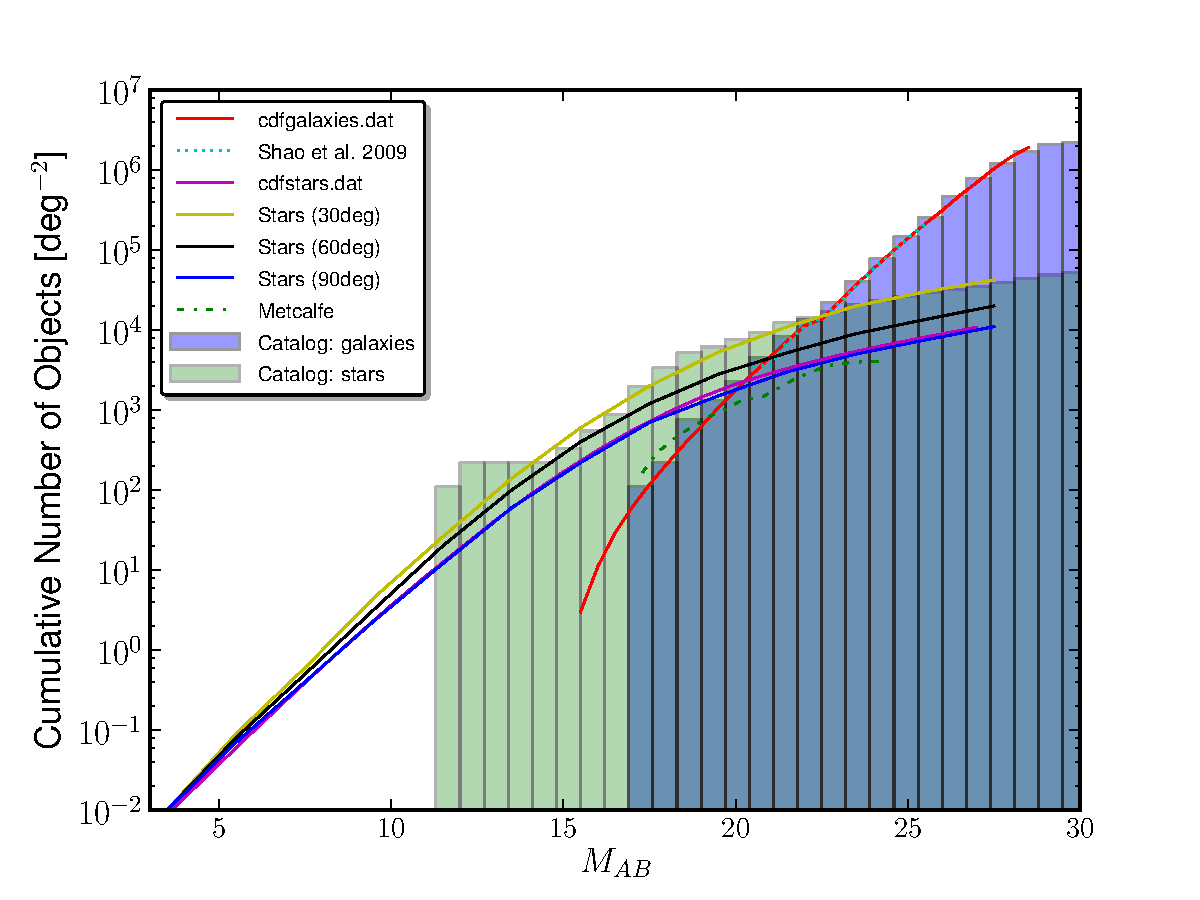
\includegraphics{Distributions.pdf}
\caption{An example showing star and galaxy number counts in a source catalog suitable for VIS simulator.
The solid lines show observations while the histograms show the distributions in the output catalogues.}\end{figure}

Another way of creating a source catalog is to use \emph{generateGalaxies} script in the \emph{simulator} subpackage.
This script depends on IRAF and uses the makeart IRAF package. There are many more options in this script,
which basically just calls the makeart's gallist and starlist. For options, see IRAF's documentation.


\chapter{Creating Simulated Mock Images}
\label{index:creating-simulated-mock-images}
The \emph{simulator} subpackage contains scripts to generate simulated VIS images. Two different methods
of generating mock images is provided. One which takes observed images (say from HST) as an input and
another in which analytical profiles are used for galaxies. The former code is custom made while the
latter relies hevily on IRAF's artdata package and mkobjects task.

The VIS reference simulator is the custom made with real observed galaxies as an input. The IRAF
based simulator can be used, for example, to train algorithms to derive elliptiticy of an object.
For more detailed documentation, please see:


\section{Simulation tools}
\label{simulator:module-simulator.simulator}\label{simulator::doc}\label{simulator:simulation-tools}\index{simulator.simulator (module)}

\subsection{The Euclid Visible Instrument Image Simulator}
\label{simulator:the-euclid-visible-instrument-image-simulator}
This file contains an image simulator for the Euclid VISible instrument.

The approximate sequence of events in the simulator is as follows:
\begin{enumerate}
\item {} 
Read in a configuration file, which defines for example,
detector characteristics (bias, dark and readout noise, gain,
plate scale and pixel scale, oversampling factor, exposure time etc.).

\item {} 
Read in another file containing charge trap definitions (for CTI modelling).

\item {} 
Read in a file defining the cosmic rays (trail lengths and cumulative distributions).

\item {} 
Read in CCD offset information, displace the image, and modify
the output file name to contain the CCD and quadrant information
(note that VIS has a focal plane of 6 x 6 detectors).

\item {} 
Read in a source list and determine the number of different object types.

\item {} 
Read in a file which assigns data to a given object index.

\item {} 
Load the PSF model (a 2D map with a given over sampling or field dependent maps).

\item {} 
Generate a finemap (oversampled image) for each object type. If an object
is a 2D image then calculate the shape tensor to be used for size scaling.
Each type of an object is then placed onto its own finely sampled finemap.

\item {} 
Loop over the number of exposures to co-add and for each object in the object catalog:
\begin{itemize}
\item {} 
determine the number of electrons an object should have by scaling the object's magnitude
with the given zeropoint and exposure time.

\item {} 
determine whether the object lands on to the detector or not and if it is
a star or an extended source (i.e. a galaxy).

\item {} 
if object is extended determine the size (using a size-magnitude relation) and scale counts,
convolve with the PSF, and finally overlay onto the detector according to its position.

\item {} 
if object is a star, scale counts according to the derived
scaling (first step), and finally overlay onto the detector according to its position.

\end{itemize}

\item {} 
Apply calibration unit flux to mimic flat field exposures {[}optional{]}.

\item {} 
Apply a multiplicative flat-field map to emulate pixel-to-pixel non-uniformity {[}optional{]}.

\item {} 
Add a charge injection line (horizontal and/or vertical) {[}optional{]}.

\item {} 
Add cosmic ray tracks onto the CCD with random positions but known distribution {[}optional{]}.

\item {} 
Apply detector charge bleeding in column direction {[}optional{]}.

\item {} 
Add constant dark current and background light from Zodiacal light {[}optional{]}.

\item {} 
Include spatially uniform scattered light to the pixel grid {[}optional{]}.

\item {} 
Add photon (Poisson) noise {[}optional{]}

\item {} 
Add cosmetic defects from an input file {[}optional{]}.

\item {} 
Add pre- and overscan regions in the serial direction {[}optional{]}.

\item {} 
Apply the CDM03 radiation damage model {[}optional{]}.

\item {} 
Apply CCD273 non-linearity model to the pixel data {[}optional{]}.

\item {} 
Add readout noise selected from a Gaussian distribution {[}optional{]}.

\item {} 
Convert from electrons to ADUs using a given gain factor.

\item {} 
Add a given bias level and discretise the counts (the output is going to be in 16bit unsigned integers).

\item {} 
Finally the simulated image is converted to a FITS file, a WCS is assigned
and the output is saved to the current working directory.

\end{enumerate}

\begin{notice}{warning}{Warning:}
The code is still work in progress and new features are being added.
The code has been tested, but nevertheless bugs may be lurking in corners, so
please report any weird or inconsistent simulations to the author.
\end{notice}


\subsubsection{Dependencies}
\label{simulator:dependencies}
This script depends on the following packages:
\begin{quote}\begin{description}
\item[{requires}] \leavevmode
PyFITS (tested with 3.0.6)

\item[{requires}] \leavevmode
NumPy (tested with 1.6.1)

\item[{requires}] \leavevmode
numexpr (tested with 2.0.1)

\item[{requires}] \leavevmode
SciPy (tested with 0.10.1)

\item[{requires}] \leavevmode
vissim-python package

\end{description}\end{quote}

\begin{notice}{note}{Note:}
This class is not Python 3 compatible. For example, xrange does not exist
in Python 3 (but is used here for speed and memory consumption improvements).
In addition, at least the string formatting should be changed if moved to
Python 3.x.
\end{notice}


\subsubsection{Testing}
\label{simulator:testing}
Before trying to run the code, please make sure that you have compiled the
cdm03.f90 Fortran code using f2py (f2py -c -m cdm03 cdm03.f90). For testing,
please run the unittest as follows:

\begin{Verbatim}[commandchars=\\\{\}]
python simulator.py -t
\end{Verbatim}

This will run the unittest and compare the result to a previously calculated image.
Please inspect the standard output for results.

Running the test will produce an image representing VIS lower left (0th) quadrant of the CCD (x, y) = (0, 0). Because
noise and cosmic rays are randomised one cannot directly compare the science
outputs but we must rely on the outputs that are free from random effects.

In the data subdirectory there is a file called ``nonoisenocrQ0\_00\_00testscience.fits'',
which is the comparison image without any noise or cosmic rays. To test the functionality,
please divide your nonoise and no cosmic ray track output image with the on in the data
folder. This should lead to a uniformly unity image or at least very close given some
numerical rounding uncertainties, especially in the FFT convolution (which is float32 not
float64).


\subsubsection{Benchmarking}
\label{simulator:benchmarking}
A minimal benchmarking has been performed using the TESTSCIENCE1X section of the test.config input file:

\begin{Verbatim}[commandchars=\\\{\}]
Galaxy: 26753/26753 magnitude=26.710577 intscale=177.489159281 FWHM=0.117285374813 arc sec
6791 objects were place on the detector

real        2m19.378s
user        2m13.237s
sys         0m4.394s
\end{Verbatim}

These numbers have been obtained with my laptop (2.2 GHz Intel Core i7) with
64-bit Python 2.7.2 installation. Further speed testing can be performed using the cProfile module
as follows:

\begin{Verbatim}[commandchars=\\\{\}]
python -m cProfile -o vissim.profile simulator.py -c data/test.config -s TESTSCIENCE3X
\end{Verbatim}

and then analysing the results with e.g. RunSnakeRun.


\subsubsection{Change Log}
\label{simulator:change-log}\begin{quote}\begin{description}
\item[{version}] \leavevmode
1.2

\end{description}\end{quote}

Version and change logs:

\begin{Verbatim}[commandchars=\\\{\}]
0.1: pre-development backbone.
0.4: first version with most pieces together.
0.5: this version has all the basic features present, but not fully tested.
0.6: implemented pre/overscan, fixed a bug when an object was getting close to the upper right corner of an
     image it was not overlaid correctly. Included multiplicative flat fielding effect (pixel non-uniformity).
0.7: implemented bleeding.
0.8: cleaned up the code and improved documentation. Fixed a bug related to checking if object falls on the CCD.
     Improved the information that is being written to the FITS header.
0.9: fixed a problem with the CTI model swapping Q1 with Q2. Fixed a bug that caused the pre- and overscan to
     be identical for each quadrant even though Q1 and 3 needs the regions to be mirrored.
1.0: First release. The code can now take an over sampled PSF and use that for convolutions. Implemented a WCS
     to the header.
1.05: included an option to add flux from the calibration unit to allow flat field exposures to be generated.
      Now scaled the number of cosmic rays with the exposure time so that 10s flats have an appropriate number
      of cosmic ray tracks.
1.06: changed how stars are laid down on the CCD. Now the PSF is interpolated to a new coordinate grid in the
      oversampled frame after which it is downsampled to the CCD grid. This should increase the centroiding
      accuracy.
1.07: included an option to apply non-linearity model. Cleaned the documentation.
1.08: optimised some of the operations with numexpr (only a minor improvement).
1.1: Fixed a bug related to adding the system readout noise. In previous versions the readout noise was
     being underestimated due to the fact that it was included as a variance not standard deviation.
1.2: Included a spatially uniform scattered light. Changed how the image pixel values are rounded before
     deriving the Poisson noise. Included focal plane CCD gaps. Included a unittest.
\end{Verbatim}


\subsubsection{Future Work}
\label{simulator:future-work}
\begin{notice}{note}{Todo}
\begin{enumerate}
\item {} 
objects.dat is now hard coded into the code, this should be read from the config file

\item {} 
implement spatially variable PSF

\item {} 
test that the WCS is correctly implemented and allows CCD offsets

\item {} 
charge injection line positions are now hardcoded to the code, read from the config file

\item {} 
include rotation in metrology

\item {} 
implement optional dithered offsets

\item {} 
try to further improve the convolution speed (look into fftw package)

\end{enumerate}
\end{notice}


\subsubsection{Contact Information}
\label{simulator:contact-information}\begin{quote}\begin{description}
\item[{author}] \leavevmode
Sami-Matias Niemi

\item[{contact}] \leavevmode
\href{mailto:s.niemi@ucl.ac.uk}{s.niemi@ucl.ac.uk}

\end{description}\end{quote}
\index{VISsimulator (class in simulator.simulator)}

\begin{fulllineitems}
\phantomsection\label{simulator:simulator.simulator.VISsimulator}\pysiglinewithargsret{\strong{class }\code{simulator.simulator.}\bfcode{VISsimulator}}{\emph{opts}}{}
Euclid Visible Instrument Image Simulator

The image that is being build is in:

\begin{Verbatim}[commandchars=\\\{\}]
\PYG{n+nb+bp}{self}\PYG{o}{.}\PYG{n}{image}
\end{Verbatim}
\begin{quote}\begin{description}
\item[{Parameters}] \leavevmode
\textbf{opts} (\emph{OptionParser instance}) -- OptionParser instance

\end{description}\end{quote}
\index{addChargeInjection() (simulator.simulator.VISsimulator method)}

\begin{fulllineitems}
\phantomsection\label{simulator:simulator.simulator.VISsimulator.addChargeInjection}\pysiglinewithargsret{\bfcode{addChargeInjection}}{}{}
Add either horizontal or vertical charge injection line to the image.

\end{fulllineitems}

\index{addCosmicRays() (simulator.simulator.VISsimulator method)}

\begin{fulllineitems}
\phantomsection\label{simulator:simulator.simulator.VISsimulator.addCosmicRays}\pysiglinewithargsret{\bfcode{addCosmicRays}}{}{}
Add cosmic rays to the arrays based on a power-law intensity distribution for tracks.

Cosmic ray properties (such as location and angle) are chosen from random Uniform distribution.

\end{fulllineitems}

\index{addLampFlux() (simulator.simulator.VISsimulator method)}

\begin{fulllineitems}
\phantomsection\label{simulator:simulator.simulator.VISsimulator.addLampFlux}\pysiglinewithargsret{\bfcode{addLampFlux}}{}{}
Include flux from the calibration source.

\end{fulllineitems}

\index{addObjects() (simulator.simulator.VISsimulator method)}

\begin{fulllineitems}
\phantomsection\label{simulator:simulator.simulator.VISsimulator.addObjects}\pysiglinewithargsret{\bfcode{addObjects}}{}{}
Add objects from the object list to the CCD image (self.image).

Scale the object's brightness in electrons and size using the input catalog magnitude.
The size-magnitude scaling relation is taken to be the equation B1 from Miller et al. 2012 (1210.8201v1;
Appendix ``prior distributions''). The spread is estimated from Figure 1 to be around 0''.1 (1 sigma).
A random draw from a Gaussian distribution with spread of 0''.1 arc sec is performed so that galaxies
of the same brightness would not be exactly the same size.

\begin{notice}{note}{Note:}
scipy.signal.fftconvolve seems to be significantly faster than scipy.signal.convolve2d.
\end{notice}

\begin{notice}{warning}{Warning:}
If random Gaussian dispersion is added to the scale-magnitude relation, then one cannot
simulate several dithers. The random dispersion can be turned off by setting random=no in
the configuration file so that dithers can be simulated and co-added correctly.
\end{notice}

\end{fulllineitems}

\index{addPreOverScans() (simulator.simulator.VISsimulator method)}

\begin{fulllineitems}
\phantomsection\label{simulator:simulator.simulator.VISsimulator.addPreOverScans}\pysiglinewithargsret{\bfcode{addPreOverScans}}{}{}
Add pre- and overscan regions to the self.image. These areas are added only in the serial direction.
Because the 1st and 3rd quadrant are read out in to a different serial direction than the nominal
orientation, in these images the regions are mirrored.

The size of prescan and overscan regions are defined by the prescanx and overscanx keywords, respectively.

\end{fulllineitems}

\index{applyBias() (simulator.simulator.VISsimulator method)}

\begin{fulllineitems}
\phantomsection\label{simulator:simulator.simulator.VISsimulator.applyBias}\pysiglinewithargsret{\bfcode{applyBias}}{}{}
Adds a bias level to the image being constructed.

The value of bias is read from the configure file and stored
in the information dictionary (key bias).

\end{fulllineitems}

\index{applyBleeding() (simulator.simulator.VISsimulator method)}

\begin{fulllineitems}
\phantomsection\label{simulator:simulator.simulator.VISsimulator.applyBleeding}\pysiglinewithargsret{\bfcode{applyBleeding}}{}{}
Apply bleeding along the CCD columns if the number of electrons in a pixel exceeds the full-well capacity.

Bleeding is modelled in the parallel direction only, because the CCD273s are assumed not to bleed in
serial direction.
\begin{quote}\begin{description}
\item[{Returns}] \leavevmode
None

\end{description}\end{quote}

\end{fulllineitems}

\index{applyCosmetics() (simulator.simulator.VISsimulator method)}

\begin{fulllineitems}
\phantomsection\label{simulator:simulator.simulator.VISsimulator.applyCosmetics}\pysiglinewithargsret{\bfcode{applyCosmetics}}{}{}
Apply cosmetic defects described in the input file.

\begin{notice}{warning}{Warning:}
This method does not work if the input file has exactly one line.
\end{notice}

\end{fulllineitems}

\index{applyDarkCurrentAndCosmicBackground() (simulator.simulator.VISsimulator method)}

\begin{fulllineitems}
\phantomsection\label{simulator:simulator.simulator.VISsimulator.applyDarkCurrentAndCosmicBackground}\pysiglinewithargsret{\bfcode{applyDarkCurrentAndCosmicBackground}}{}{}
Apply dark current and the cosmic background.
Scales dark and background with the exposure time.

Additionally saves the image without noise to a FITS file.

\end{fulllineitems}

\index{applyFlatfield() (simulator.simulator.VISsimulator method)}

\begin{fulllineitems}
\phantomsection\label{simulator:simulator.simulator.VISsimulator.applyFlatfield}\pysiglinewithargsret{\bfcode{applyFlatfield}}{}{}
Applies multiplicative flat field to emulate pixel-to-pixel non-uniformity.

Because the pixel-to-pixel non-uniformity effect (i.e. multiplicative) flat fielding takes place
before CTI and other effects, the flat field file must be the same size as the pixels that see
the sky. Thus, in case of a single quadrant (x, y) = (2048, 2066).

\end{fulllineitems}

\index{applyNonlinearity() (simulator.simulator.VISsimulator method)}

\begin{fulllineitems}
\phantomsection\label{simulator:simulator.simulator.VISsimulator.applyNonlinearity}\pysiglinewithargsret{\bfcode{applyNonlinearity}}{}{}
Applies a CCD273 non-linearity model to the image being constructed.

\end{fulllineitems}

\index{applyPoissonNoise() (simulator.simulator.VISsimulator method)}

\begin{fulllineitems}
\phantomsection\label{simulator:simulator.simulator.VISsimulator.applyPoissonNoise}\pysiglinewithargsret{\bfcode{applyPoissonNoise}}{}{}
Add Poisson noise to the image.

\end{fulllineitems}

\index{applyRadiationDamage() (simulator.simulator.VISsimulator method)}

\begin{fulllineitems}
\phantomsection\label{simulator:simulator.simulator.VISsimulator.applyRadiationDamage}\pysiglinewithargsret{\bfcode{applyRadiationDamage}}{}{}
Applies CDM03 radiation model to the image being constructed.


\strong{See Also:}


Class :\emph{CDM03}



\end{fulllineitems}

\index{applyReadoutNoise() (simulator.simulator.VISsimulator method)}

\begin{fulllineitems}
\phantomsection\label{simulator:simulator.simulator.VISsimulator.applyReadoutNoise}\pysiglinewithargsret{\bfcode{applyReadoutNoise}}{}{}
Applies readout noise to the image being constructed.

The noise is drawn from a Normal (Gaussian) distribution with average=0.0 and std=readout noise.

\end{fulllineitems}

\index{applyScatteredLight() (simulator.simulator.VISsimulator method)}

\begin{fulllineitems}
\phantomsection\label{simulator:simulator.simulator.VISsimulator.applyScatteredLight}\pysiglinewithargsret{\bfcode{applyScatteredLight}}{}{}
Adds spatially uniform scattered light to the image.

\end{fulllineitems}

\index{configure() (simulator.simulator.VISsimulator method)}

\begin{fulllineitems}
\phantomsection\label{simulator:simulator.simulator.VISsimulator.configure}\pysiglinewithargsret{\bfcode{configure}}{}{}
Configures the simulator with input information and creates and empty array to which the final image will
be build on.

\end{fulllineitems}

\index{cosmicRayIntercepts() (simulator.simulator.VISsimulator method)}

\begin{fulllineitems}
\phantomsection\label{simulator:simulator.simulator.VISsimulator.cosmicRayIntercepts}\pysiglinewithargsret{\bfcode{cosmicRayIntercepts}}{\emph{lum}, \emph{x0}, \emph{y0}, \emph{l}, \emph{phi}}{}
Derive cosmic ray streak intercept points.
\begin{quote}\begin{description}
\item[{Parameters}] \leavevmode\begin{itemize}
\item {} 
\textbf{lum} -- luminosities of the cosmic ray tracks

\item {} 
\textbf{x0} -- central positions of the cosmic ray tracks in x-direction

\item {} 
\textbf{y0} -- central positions of the cosmic ray tracks in y-direction

\item {} 
\textbf{l} -- lengths of the cosmic ray tracks

\item {} 
\textbf{phi} -- orientation angles of the cosmic ray tracks

\end{itemize}

\item[{Returns}] \leavevmode
map

\item[{Return type}] \leavevmode
nd-array

\end{description}\end{quote}

\end{fulllineitems}

\index{discretise() (simulator.simulator.VISsimulator method)}

\begin{fulllineitems}
\phantomsection\label{simulator:simulator.simulator.VISsimulator.discretise}\pysiglinewithargsret{\bfcode{discretise}}{\emph{max=65535}}{}
Converts a floating point image array (self.image) to an integer array with max values
defined by the argument max.
\begin{quote}\begin{description}
\item[{Parameters}] \leavevmode
\textbf{max} (\emph{float}) -- maximum value the the integer array may contain {[}default 65k{]}

\item[{Returns}] \leavevmode
None

\end{description}\end{quote}

\end{fulllineitems}

\index{electrons2ADU() (simulator.simulator.VISsimulator method)}

\begin{fulllineitems}
\phantomsection\label{simulator:simulator.simulator.VISsimulator.electrons2ADU}\pysiglinewithargsret{\bfcode{electrons2ADU}}{}{}
Convert from electrons to ADUs using the value read from the configuration file.

\end{fulllineitems}

\index{generateFinemaps() (simulator.simulator.VISsimulator method)}

\begin{fulllineitems}
\phantomsection\label{simulator:simulator.simulator.VISsimulator.generateFinemaps}\pysiglinewithargsret{\bfcode{generateFinemaps}}{}{}
Generates finely sampled images of the input data.

\end{fulllineitems}

\index{objectOnDetector() (simulator.simulator.VISsimulator method)}

\begin{fulllineitems}
\phantomsection\label{simulator:simulator.simulator.VISsimulator.objectOnDetector}\pysiglinewithargsret{\bfcode{objectOnDetector}}{\emph{object}}{}
Tests if the object falls on the detector.
\begin{quote}\begin{description}
\item[{Parameters}] \leavevmode
\textbf{object} -- object to be placed to the self.image.

\item[{Returns}] \leavevmode
whether the object falls on the detector or not

\item[{Return type}] \leavevmode
boolean

\end{description}\end{quote}

\end{fulllineitems}

\index{overlayToCCD() (simulator.simulator.VISsimulator method)}

\begin{fulllineitems}
\phantomsection\label{simulator:simulator.simulator.VISsimulator.overlayToCCD}\pysiglinewithargsret{\bfcode{overlayToCCD}}{\emph{data}, \emph{obj}}{}
Overlay data from a source object onto the self.image.
\begin{quote}\begin{description}
\item[{Parameters}] \leavevmode\begin{itemize}
\item {} 
\textbf{data} (\emph{ndarray}) -- ndarray of data to be overlaid on to self.image

\item {} 
\textbf{obj} (\emph{list}) -- object information such as x,y position

\end{itemize}

\end{description}\end{quote}

\end{fulllineitems}

\index{processConfigs() (simulator.simulator.VISsimulator method)}

\begin{fulllineitems}
\phantomsection\label{simulator:simulator.simulator.VISsimulator.processConfigs}\pysiglinewithargsret{\bfcode{processConfigs}}{}{}
Processes configuration information and save the information to a dictionary self.information.

The configuration file may look as follows:

\begin{Verbatim}[commandchars=\\\{\}]
\PYG{p}{[}\PYG{n}{TEST}\PYG{p}{]}
\PYG{n}{quadrant} \PYG{o}{=} \PYG{l+m+mi}{0}
\PYG{n}{CCDx} \PYG{o}{=} \PYG{l+m+mi}{0}
\PYG{n}{CCDy} \PYG{o}{=} \PYG{l+m+mi}{0}
\PYG{n}{CCDxgap} \PYG{o}{=} \PYG{l+m+mf}{1.643}
\PYG{n}{CCDygap} \PYG{o}{=} \PYG{l+m+mf}{8.116}
\PYG{n}{xsize} \PYG{o}{=} \PYG{l+m+mi}{2048}
\PYG{n}{ysize} \PYG{o}{=} \PYG{l+m+mi}{2066}
\PYG{n}{prescanx} \PYG{o}{=} \PYG{l+m+mi}{50}
\PYG{n}{ovrscanx} \PYG{o}{=} \PYG{l+m+mi}{20}
\PYG{n}{fullwellcapacity} \PYG{o}{=} \PYG{l+m+mi}{200000}
\PYG{n}{dark} \PYG{o}{=} \PYG{l+m+mf}{0.001}
\PYG{n}{readout} \PYG{o}{=} \PYG{l+m+mf}{4.5}
\PYG{n}{bias} \PYG{o}{=} \PYG{l+m+mf}{1000.0}
\PYG{n}{cosmic\PYGZus{}bkgd} \PYG{o}{=} \PYG{l+m+mf}{0.182758225257}
\PYG{n}{e\PYGZus{}ADU} \PYG{o}{=} \PYG{l+m+mf}{3.1}
\PYG{n}{injection} \PYG{o}{=} \PYG{l+m+mf}{150000.0}
\PYG{n}{magzero} \PYG{o}{=} \PYG{l+m+mf}{15182880871.225231}
\PYG{n}{exposures} \PYG{o}{=} \PYG{l+m+mi}{1}
\PYG{n}{exptime} \PYG{o}{=} \PYG{l+m+mf}{565.0}
\PYG{n}{RA} \PYG{o}{=} \PYG{l+m+mf}{145.95}
\PYG{n}{DEC} \PYG{o}{=} \PYG{o}{\PYGZhy{}}\PYG{l+m+mf}{38.16}
\PYG{n}{sourcelist} \PYG{o}{=} \PYG{n}{data}\PYG{o}{/}\PYG{n}{source\PYGZus{}test}\PYG{o}{.}\PYG{n}{dat}
\PYG{n}{PSFfile} \PYG{o}{=} \PYG{n}{data}\PYG{o}{/}\PYG{n}{interpolated\PYGZus{}psf}\PYG{o}{.}\PYG{n}{fits}
\PYG{n}{trapfile} \PYG{o}{=} \PYG{n}{data}\PYG{o}{/}\PYG{n}{cdm\PYGZus{}euclid}\PYG{o}{.}\PYG{n}{dat}
\PYG{n}{cosmeticsFile} \PYG{o}{=} \PYG{n}{data}\PYG{o}{/}\PYG{n}{cosmetics}\PYG{o}{.}\PYG{n}{dat}
\PYG{n}{flatfieldfile} \PYG{o}{=} \PYG{n}{data}\PYG{o}{/}\PYG{n}{VISFlatField2percent}\PYG{o}{.}\PYG{n}{fits}
\PYG{n}{output} \PYG{o}{=} \PYG{n}{test}\PYG{o}{.}\PYG{n}{fits}
\PYG{n}{addSources} \PYG{o}{=} \PYG{n}{yes}
\PYG{n}{noise} \PYG{o}{=} \PYG{n}{yes}
\PYG{n}{cosmetics} \PYG{o}{=} \PYG{n}{no}
\PYG{n}{chargeInjectionx} \PYG{o}{=} \PYG{n}{no}
\PYG{n}{chargeInjectiony} \PYG{o}{=} \PYG{n}{no}
\PYG{n}{radiationDamage} \PYG{o}{=} \PYG{n}{yes}
\PYG{n}{cosmicRays} \PYG{o}{=} \PYG{n}{yes}
\PYG{n}{overscans} \PYG{o}{=} \PYG{n}{yes}
\PYG{n}{bleeding} \PYG{o}{=} \PYG{n}{yes}
\PYG{n}{flatfieldM} \PYG{o}{=} \PYG{n}{yes}
\PYG{n}{random} \PYG{o}{=} \PYG{n}{yes}
\end{Verbatim}

For explanation of each field, see /data/test.config. Note that if an input field does not exist,
then the values are taken from the default instrument model as described in
support.VISinstrumentModel.VISinformation(). Any of the defaults can be overwritten by providing
a config file with a correct field name.

\end{fulllineitems}

\index{readConfigs() (simulator.simulator.VISsimulator method)}

\begin{fulllineitems}
\phantomsection\label{simulator:simulator.simulator.VISsimulator.readConfigs}\pysiglinewithargsret{\bfcode{readConfigs}}{}{}
Reads the config file information using configParser.

\end{fulllineitems}

\index{readCosmicRayInformation() (simulator.simulator.VISsimulator method)}

\begin{fulllineitems}
\phantomsection\label{simulator:simulator.simulator.VISsimulator.readCosmicRayInformation}\pysiglinewithargsret{\bfcode{readCosmicRayInformation}}{}{}
Reads in the cosmic ray track information from two input files.

Stores the information to a dictionary called cr.

\end{fulllineitems}

\index{readObjectlist() (simulator.simulator.VISsimulator method)}

\begin{fulllineitems}
\phantomsection\label{simulator:simulator.simulator.VISsimulator.readObjectlist}\pysiglinewithargsret{\bfcode{readObjectlist}}{}{}
Reads object list using numpy.loadtxt, determines the number of object types,
and finds the file that corresponds to a given object type.

The input catalog is assumed to contain the following columns:
\begin{enumerate}
\item {} 
x coordinate

\item {} 
y coordinate

\item {} 
apparent magnitude of the object

\item {} 
type of the object {[}0=star, number=type defined in the objects.dat{]}

\item {} 
rotation {[}0 for stars, {[}0, 360{]} for galaxies{]}

\end{enumerate}

This method also displaces the object coordinates based on the quadrant and the
CCD to be simulated.

\begin{notice}{note}{Note:}
If even a single object type does not have a corresponding input then this method
forces the program to exit.
\end{notice}

\end{fulllineitems}

\index{readPSFs() (simulator.simulator.VISsimulator method)}

\begin{fulllineitems}
\phantomsection\label{simulator:simulator.simulator.VISsimulator.readPSFs}\pysiglinewithargsret{\bfcode{readPSFs}}{}{}
Reads in a PSF from a FITS file.

\begin{notice}{note}{Note:}
at the moment this method supports only a single PSF file.
\end{notice}

\end{fulllineitems}

\index{simulate() (simulator.simulator.VISsimulator method)}

\begin{fulllineitems}
\phantomsection\label{simulator:simulator.simulator.VISsimulator.simulate}\pysiglinewithargsret{\bfcode{simulate}}{}{}
Create a single simulated image of a quadrant defined by the configuration file.
Will do all steps defined in the config file sequentially.
\begin{quote}\begin{description}
\item[{Returns}] \leavevmode
None

\end{description}\end{quote}

\end{fulllineitems}

\index{writeFITSfile() (simulator.simulator.VISsimulator method)}

\begin{fulllineitems}
\phantomsection\label{simulator:simulator.simulator.VISsimulator.writeFITSfile}\pysiglinewithargsret{\bfcode{writeFITSfile}}{\emph{data}, \emph{filename}, \emph{unsigned16bit=False}}{}
Writes out a simple FITS file.
\begin{quote}\begin{description}
\item[{Parameters}] \leavevmode\begin{itemize}
\item {} 
\textbf{data} (\emph{ndarray}) -- data to be written

\item {} 
\textbf{filename} (\emph{str}) -- name of the output file

\item {} 
\textbf{unsigned16bit} (\emph{bool}) -- whether to scale the data using bzero=32768

\end{itemize}

\item[{Returns}] \leavevmode
None

\end{description}\end{quote}

\end{fulllineitems}

\index{writeOutputs() (simulator.simulator.VISsimulator method)}

\begin{fulllineitems}
\phantomsection\label{simulator:simulator.simulator.VISsimulator.writeOutputs}\pysiglinewithargsret{\bfcode{writeOutputs}}{}{}
Writes out a FITS file using PyFITS and converts the image array to 16bit unsigned integer as
appropriate for VIS.

Updates header with the input values and flags used during simulation.

\end{fulllineitems}


\end{fulllineitems}

\phantomsection\label{simulator:module-simulator.generateGalaxies}\index{simulator.generateGalaxies (module)}

\subsection{Generating Mock Objects with IRAF}
\label{simulator:generating-mock-objects-with-iraf}
This script provides a class that can be used to generate objects such as galaxies using IRAF.
\begin{quote}\begin{description}
\item[{requires}] \leavevmode
PyRAF

\item[{requires}] \leavevmode
PyFITS

\item[{requires}] \leavevmode
NumPy

\item[{author}] \leavevmode
Sami-Matias Niemi

\item[{contact}] \leavevmode
\href{mailto:smn2@mssl.ucl.ac.uk}{smn2@mssl.ucl.ac.uk}

\item[{version}] \leavevmode
0.1

\end{description}\end{quote}
\index{generateFakeData (class in simulator.generateGalaxies)}

\begin{fulllineitems}
\phantomsection\label{simulator:simulator.generateGalaxies.generateFakeData}\pysiglinewithargsret{\strong{class }\code{simulator.generateGalaxies.}\bfcode{generateFakeData}}{\emph{log}, \emph{**kwargs}}{}
Generates an image frame with stars and galaxies using IRAF's artdata.
\index{addObjects() (simulator.generateGalaxies.generateFakeData method)}

\begin{fulllineitems}
\phantomsection\label{simulator:simulator.generateGalaxies.generateFakeData.addObjects}\pysiglinewithargsret{\bfcode{addObjects}}{\emph{inputlist='galaxies.dat'}}{}
Add object(s) from inputlist to the output image.
\begin{quote}\begin{description}
\item[{Parameters}] \leavevmode
\textbf{inputlist} (\emph{str}) -- name of the input list

\end{description}\end{quote}

\end{fulllineitems}

\index{createGalaxylist() (simulator.generateGalaxies.generateFakeData method)}

\begin{fulllineitems}
\phantomsection\label{simulator:simulator.generateGalaxies.generateFakeData.createGalaxylist}\pysiglinewithargsret{\bfcode{createGalaxylist}}{\emph{ngalaxies=150}, \emph{output='galaxies.dat'}}{}
Generates an ascii file with uniform random x and y positions.
The magnitudes of galaxies are taken from an isotropic and homogeneous power-law distribution.

The output ascii file contains the following columns: xc yc magnitude model radius ar pa \textless{}save\textgreater{}
\begin{quote}\begin{description}
\item[{Parameters}] \leavevmode\begin{itemize}
\item {} 
\textbf{ngalaxies} (\emph{int}) -- number of galaxies to include

\item {} 
\textbf{output} (\emph{str}) -- name of the output ascii file

\end{itemize}

\end{description}\end{quote}

\end{fulllineitems}

\index{createStarlist() (simulator.generateGalaxies.generateFakeData method)}

\begin{fulllineitems}
\phantomsection\label{simulator:simulator.generateGalaxies.generateFakeData.createStarlist}\pysiglinewithargsret{\bfcode{createStarlist}}{\emph{nstars=20}, \emph{output='stars.dat'}}{}
Generates an ascii file with uniform random x and y positions.
The magnitudes of stars are taken from an isotropic and homogeneous power-law distribution.

The output ascii file contains the following columns: xc yc magnitude
\begin{quote}\begin{description}
\item[{Parameters}] \leavevmode\begin{itemize}
\item {} 
\textbf{nstars} (\emph{int}) -- number of stars to include

\item {} 
\textbf{output} (\emph{str}) -- name of the output ascii file

\end{itemize}

\end{description}\end{quote}

\end{fulllineitems}

\index{maskCrazyValues() (simulator.generateGalaxies.generateFakeData method)}

\begin{fulllineitems}
\phantomsection\label{simulator:simulator.generateGalaxies.generateFakeData.maskCrazyValues}\pysiglinewithargsret{\bfcode{maskCrazyValues}}{\emph{filename=None}}{}
For some reason mkobjects sometimes adds crazy values to an image.
This method tries to remove those values and set them to more reasonable ones.
The values \textgreater{} 65k are set to the median of the image.
\begin{quote}\begin{description}
\item[{Parameters}] \leavevmode
\textbf{filename} (\emph{str}) -- name of the input file to modify {[}default = self.settings{[}'output'{]}{]}

\item[{Returns}] \leavevmode
None

\end{description}\end{quote}

\end{fulllineitems}

\index{runAll() (simulator.generateGalaxies.generateFakeData method)}

\begin{fulllineitems}
\phantomsection\label{simulator:simulator.generateGalaxies.generateFakeData.runAll}\pysiglinewithargsret{\bfcode{runAll}}{\emph{nostars=True}}{}
Run all methods sequentially.

\end{fulllineitems}


\end{fulllineitems}

\begin{figure}[htbp]
\centering
\capstart

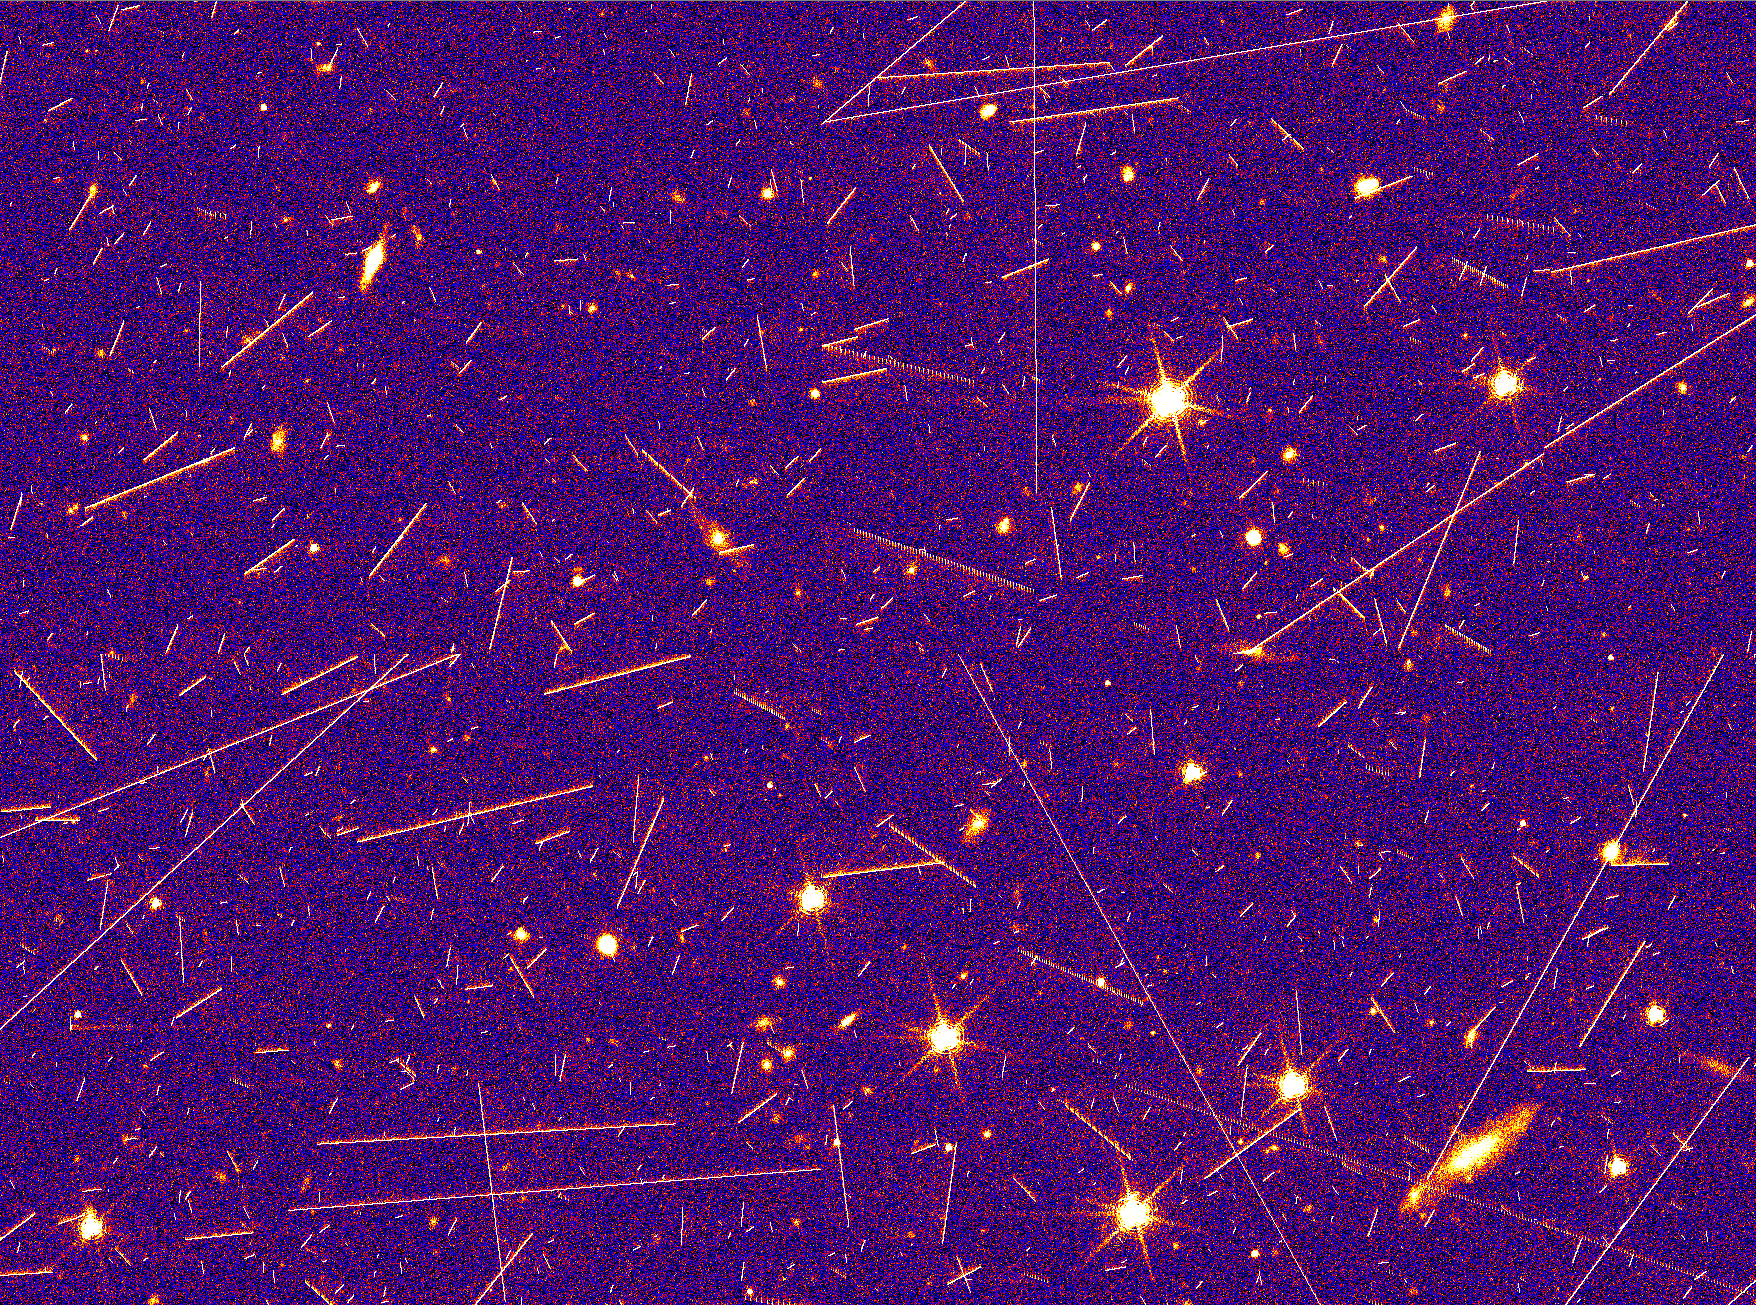
\includegraphics{VISpartOfCCDlogscale.png}
\caption{An example image generated with the VIS simulator. The image shows a part of a single
CCD. The image is on a logarithmic stretch.}\end{figure}
\begin{figure}[htbp]
\centering
\capstart

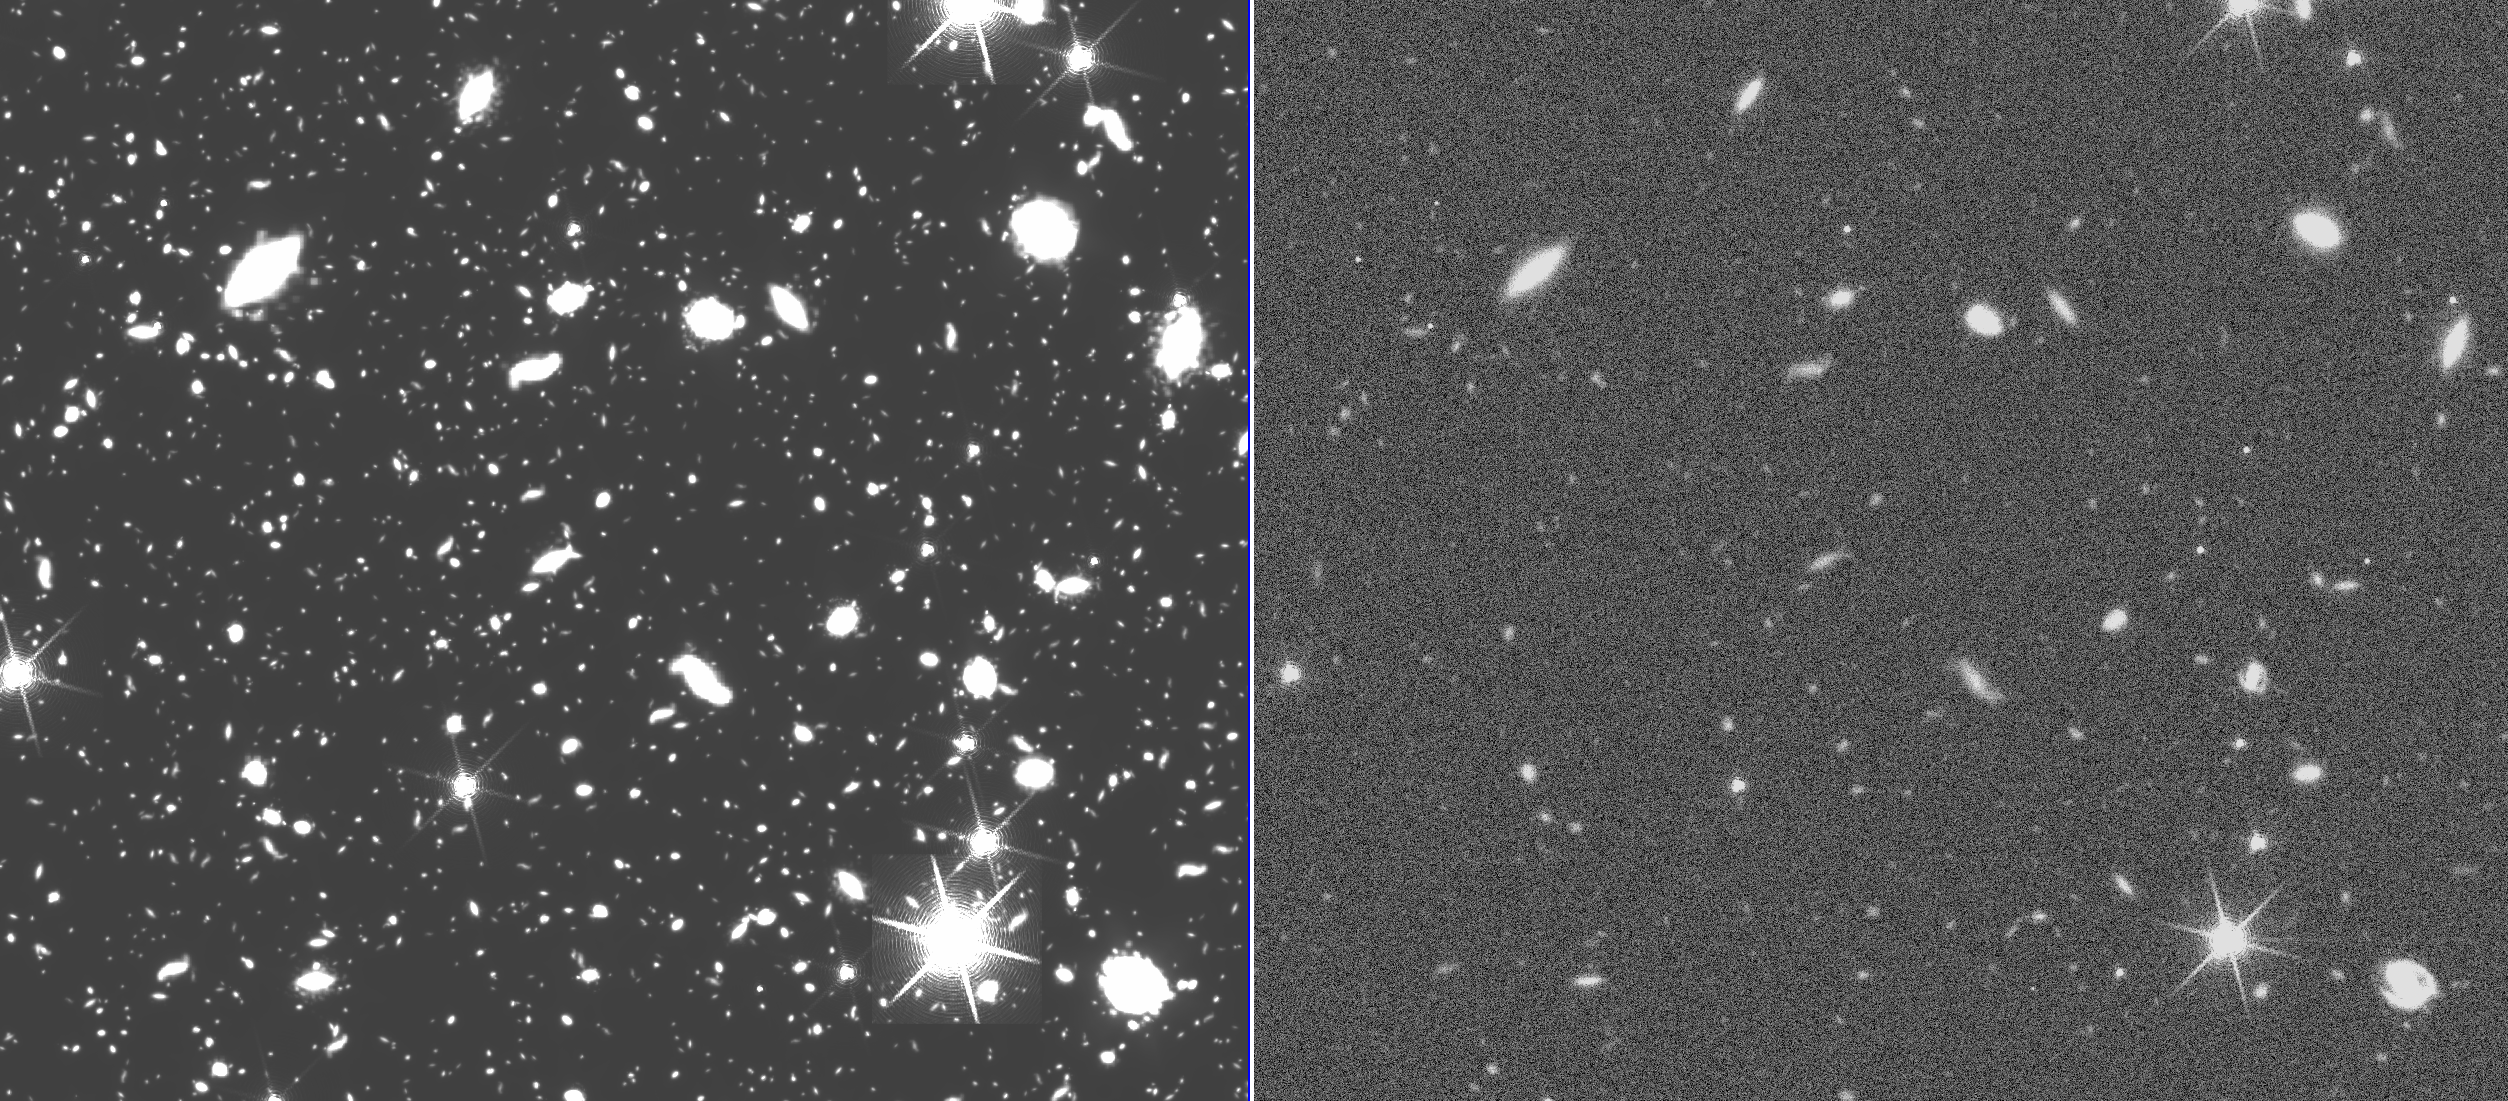
\includegraphics{noisecomparison.png}
\caption{A simulated image with no noise (left) and with noise (right). The simulated image with noise
includes: Zodiacal background, scattered light, readout and Poisson noise, CTI, etc. Both images
are on logarithmic stretch.}\end{figure}
\begin{figure}[htbp]
\centering
\capstart

\includegraphics{VISImage.png}
\caption{Full focal plane of VIS with zoom-in sections. The data were generated with the VIS simulator. The data
are on log-scale.}\end{figure}


\chapter{Data reduction}
\label{index:data-reduction}
The \emph{reduction} subpackage contains a simple script to reduce VIS data. For more detailed documentation
of the classes, please see:


\section{Data reduction tools}
\label{reduction:module-reduction.reduceVISdata}\label{reduction::doc}\label{reduction:data-reduction-tools}\index{reduction.reduceVISdata (module)}

\subsection{VIS Data Reduction and Processing}
\label{reduction:vis-data-reduction-and-processing}
This simple script can be used to reduce (simulated) VIS data.

The script was initially written for reducing a single CCD data.
However, since the version 0.5 the script tries to guess if the
input is a single quadrant then reduce correctly.

The script performs the following data reduction steps:

\begin{Verbatim}[commandchars=\\\{\}]
1 Bias correction
2 CTI correction
3 Flat fielding (only if an input file is provided)
\end{Verbatim}

To Run:

\begin{Verbatim}[commandchars=\\\{\}]
python reduceVISdata.py -i VISCCD.fits -b superBiasVIS.fits -f SuperFlatField.fits
\end{Verbatim}
\begin{quote}\begin{description}
\item[{requires}] \leavevmode
PyFITS

\item[{requires}] \leavevmode
NumPy

\item[{requires}] \leavevmode
CDM03 (FORTRAN code, f2py -c -m cdm03 cdm03.f90)

\item[{author}] \leavevmode
Sami-Matias Niemi

\item[{contact}] \leavevmode
\href{mailto:smn2@mssl.ucl.ac.uk}{smn2@mssl.ucl.ac.uk}

\item[{version}] \leavevmode
0.5

\end{description}\end{quote}

\begin{notice}{note}{Todo}
\begin{enumerate}
\item {} 
implement background/sky subtraction

\end{enumerate}
\end{notice}
\index{reduceVISdata (class in reduction.reduceVISdata)}

\begin{fulllineitems}
\phantomsection\label{reduction:reduction.reduceVISdata.reduceVISdata}\pysiglinewithargsret{\strong{class }\code{reduction.reduceVISdata.}\bfcode{reduceVISdata}}{\emph{values}, \emph{log}}{}
Simple class to reduce VIS data.
\index{applyCTICorrection() (reduction.reduceVISdata.reduceVISdata method)}

\begin{fulllineitems}
\phantomsection\label{reduction:reduction.reduceVISdata.reduceVISdata.applyCTICorrection}\pysiglinewithargsret{\bfcode{applyCTICorrection}}{}{}
Applies a CTI correction in electrons using CDM03 CTI model.
Converts the data to electrons using the gain value given in self.values.
The number of forward reads is defined by self.values{[}'order'{]} parameter.

Bristow \& Alexov (2003) algorithm further developed for HST data
processing by Massey, Rhodes et al.

There is probably an excess of .copy() calls here, but I had some problems
when calling the Fortran code so I added them for now.

\end{fulllineitems}

\index{flatfield() (reduction.reduceVISdata.reduceVISdata method)}

\begin{fulllineitems}
\phantomsection\label{reduction:reduction.reduceVISdata.reduceVISdata.flatfield}\pysiglinewithargsret{\bfcode{flatfield}}{}{}
Take into account pixel-to-pixel non-uniformity through multiplicative flat fielding.

\end{fulllineitems}

\index{subtractBias() (reduction.reduceVISdata.reduceVISdata method)}

\begin{fulllineitems}
\phantomsection\label{reduction:reduction.reduceVISdata.reduceVISdata.subtractBias}\pysiglinewithargsret{\bfcode{subtractBias}}{}{}
Simply subtracts self.bias from the input data.

\end{fulllineitems}

\index{writeFITSfile() (reduction.reduceVISdata.reduceVISdata method)}

\begin{fulllineitems}
\phantomsection\label{reduction:reduction.reduceVISdata.reduceVISdata.writeFITSfile}\pysiglinewithargsret{\bfcode{writeFITSfile}}{}{}
Write out FITS files using PyFITS.

\end{fulllineitems}


\end{fulllineitems}



\section{VIS data reduction studies}
\label{reduction:vis-data-reduction-studies}\label{reduction:module-analysis.biasCalibration}\index{analysis.biasCalibration (module)}

\subsection{Bias Calibration}
\label{reduction:bias-calibration}
This simple script can be used to study the number of bias frames required to meet the VIS calibration requirements.

The following requirements related to the bias calibration has been taken from GDPRD.

R-GDP-CAL-052:
The contribution of the residuals of VIS bias subtraction to the \emph{error on the determination of each ellipticity
component} of the local PSF shall not exceed 3x10-5 (one sigma).

R-GDP-CAL-062:
The contribution of the residuals of VIS bias subtraction to the \emph{relative error} sigma(R2)/R2 on the determination of
the local PSF R2 shall not exceed 1x10-4 (one sigma).
\begin{quote}\begin{description}
\item[{requires}] \leavevmode
PyFITS

\item[{requires}] \leavevmode
NumPy

\item[{requires}] \leavevmode
matplotlib

\item[{requires}] \leavevmode
VISsim-Python

\item[{version}] \leavevmode
0.95

\item[{author}] \leavevmode
Sami-Matias Niemi

\item[{contact}] \leavevmode
\href{mailto:smn2@mssl.ucl.ac.uk}{smn2@mssl.ucl.ac.uk}

\end{description}\end{quote}
\index{addReadoutNoise() (in module analysis.biasCalibration)}

\begin{fulllineitems}
\phantomsection\label{reduction:analysis.biasCalibration.addReadoutNoise}\pysiglinewithargsret{\code{analysis.biasCalibration.}\bfcode{addReadoutNoise}}{\emph{data}, \emph{readnoise=4.5}, \emph{gain=3.1}, \emph{number=1}}{}
Add readout noise to the input data. The readout noise is the median of the number of frames.
\begin{quote}\begin{description}
\item[{Parameters}] \leavevmode\begin{itemize}
\item {} 
\textbf{data} (\emph{ndarray}) -- input data to which the readout noise will be added to {[}ADUs{]}

\item {} 
\textbf{readnoise} (\emph{float}) -- standard deviation of the read out noise {[}electrons{]}

\item {} 
\textbf{gain} (\emph{float}) -- the gain factor that is used to convert electrons to ADUs

\item {} 
\textbf{number} (\emph{int}) -- number of read outs to median combine before adding to the data {[}default=1{]}

\end{itemize}

\item[{Returns}] \leavevmode
data + read out noise

\item[{Return type}] \leavevmode
ndarray {[}same as input data{]}

\end{description}\end{quote}

\end{fulllineitems}

\index{findTolerableErrorPiston() (in module analysis.biasCalibration)}

\begin{fulllineitems}
\phantomsection\label{reduction:analysis.biasCalibration.findTolerableErrorPiston}\pysiglinewithargsret{\code{analysis.biasCalibration.}\bfcode{findTolerableErrorPiston}}{\emph{log}, \emph{file='data/psf12x.fits'}, \emph{oversample=12.0}, \emph{samples=12}, \emph{psfs=4000}, \emph{sigma=0.36}, \emph{iterations=5}, \emph{debug=False}}{}
Calculate ellipticity and size for PSFs of different scaling when there is a residual
bias offset.
\begin{quote}\begin{description}
\item[{Parameters}] \leavevmode
\textbf{sigma} (\emph{float}) -- 1sigma radius of the Gaussian weighting function for shape measurements

\end{description}\end{quote}

\end{fulllineitems}

\index{findTolerableErrorSlope() (in module analysis.biasCalibration)}

\begin{fulllineitems}
\phantomsection\label{reduction:analysis.biasCalibration.findTolerableErrorSlope}\pysiglinewithargsret{\code{analysis.biasCalibration.}\bfcode{findTolerableErrorSlope}}{\emph{log}, \emph{file='data/psf12x.fits'}, \emph{oversample=12.0}, \emph{samples=12}, \emph{psfs=4000}, \emph{sigma=0.36}, \emph{iterations=5}, \emph{pixels=60}}{}
Calculate ellipticity and size for PSFs of different scaling when there is a residual
bias slope.
\begin{quote}\begin{description}
\item[{Parameters}] \leavevmode
\textbf{sigma} (\emph{float}) -- 1sigma radius of the Gaussian weighting function for shape measurements

\end{description}\end{quote}

\end{fulllineitems}

\index{pistonKnowledge() (in module analysis.biasCalibration)}

\begin{fulllineitems}
\phantomsection\label{reduction:analysis.biasCalibration.pistonKnowledge}\pysiglinewithargsret{\code{analysis.biasCalibration.}\bfcode{pistonKnowledge}}{\emph{log}, \emph{file='data/psf2x.fits'}, \emph{oversample=2.0}, \emph{psfs=1000}, \emph{sigma=0.36}, \emph{iterations=4}, \emph{debug=False}}{}
\end{fulllineitems}

\index{plotDeltaEs() (in module analysis.biasCalibration)}

\begin{fulllineitems}
\phantomsection\label{reduction:analysis.biasCalibration.plotDeltaEs}\pysiglinewithargsret{\code{analysis.biasCalibration.}\bfcode{plotDeltaEs}}{\emph{deltae1}, \emph{deltae2}, \emph{deltae}, \emph{output}, \emph{title='`}, \emph{ymax=8}, \emph{req=3}}{}
Generates a simple plot showing the errors in the ellipticity components.

\end{fulllineitems}

\index{plotEs() (in module analysis.biasCalibration)}

\begin{fulllineitems}
\phantomsection\label{reduction:analysis.biasCalibration.plotEs}\pysiglinewithargsret{\code{analysis.biasCalibration.}\bfcode{plotEs}}{\emph{deltae1}, \emph{deltae2}, \emph{deltae}, \emph{output}, \emph{title='`}}{}
Generates a simple plot showing the ellipticity components.

\end{fulllineitems}

\index{plotNumberOfFramesDelta() (in module analysis.biasCalibration)}

\begin{fulllineitems}
\phantomsection\label{reduction:analysis.biasCalibration.plotNumberOfFramesDelta}\pysiglinewithargsret{\code{analysis.biasCalibration.}\bfcode{plotNumberOfFramesDelta}}{\emph{results}, \emph{timeStamp=False}}{}
Creates a simple plot to combine and show the results for errors (delta).
\begin{quote}\begin{description}
\item[{Parameters}] \leavevmode\begin{itemize}
\item {} 
\textbf{results} (\emph{dict}) -- results to be plotted

\item {} 
\textbf{timeStamp} (\emph{bool}) -- whether to include a time stamp in the output image

\end{itemize}

\end{description}\end{quote}

\end{fulllineitems}

\index{plotNumberOfFramesSigma() (in module analysis.biasCalibration)}

\begin{fulllineitems}
\phantomsection\label{reduction:analysis.biasCalibration.plotNumberOfFramesSigma}\pysiglinewithargsret{\code{analysis.biasCalibration.}\bfcode{plotNumberOfFramesSigma}}{\emph{results}, \emph{reqe=3e-05}, \emph{reqr2=0.0001}, \emph{shift=0.1}, \emph{timeStamp=False}}{}
Creates a simple plot to combine and show the results.
\begin{quote}\begin{description}
\item[{Parameters}] \leavevmode\begin{itemize}
\item {} 
\textbf{results} (\emph{dict}) -- results to be plotted

\item {} 
\textbf{req} (\emph{float}) -- the requirement

\item {} 
\textbf{ymax} (\emph{int or float}) -- maximum value to show on the y-axis

\item {} 
\textbf{shift} (\emph{float}) -- the amount to shift the e2 results on the abscissa (for clarity)

\item {} 
\textbf{timeStamp} (\emph{bool}) -- whether to include a time stamp in the output image

\end{itemize}

\end{description}\end{quote}

\end{fulllineitems}

\index{testBiasCalibrationDelta() (in module analysis.biasCalibration)}

\begin{fulllineitems}
\phantomsection\label{reduction:analysis.biasCalibration.testBiasCalibrationDelta}\pysiglinewithargsret{\code{analysis.biasCalibration.}\bfcode{testBiasCalibrationDelta}}{\emph{log}, \emph{numdata=2066}, \emph{floor=995}, \emph{xsize=2048}, \emph{ysize=2066}, \emph{order=3}, \emph{biases=15}, \emph{surfaces=100}, \emph{file='psf1x.fits'}, \emph{psfs=500}, \emph{psfscale=1000.0}, \emph{debug=False}, \emph{plots=False}}{}
Derive the PSF ellipticities for a given number of random surfaces with random PSF positions
and a given number of biases median combined and compare to the nominal PSF ellipticity.

This function can be used to derive the error (delta) in determining ellipticity and size given
a reference PSF.

Choices that need to be made and effect the results:
\begin{enumerate}
\item {} 
bias surface that is assumed (amplitude, complexity, etc.)

\item {} 
whether the order of the polynomial surface to be fitted is known or not

\item {} 
size of the Gaussian weighting function when calculating the ellipticity components

\end{enumerate}

There are also other choices such as the number of PSFs and scaling and the random numbers generated for
the surface that also affect the results, however, to a lesser degree.

Generates a set of plots that can be used to inspect the simulation.

\end{fulllineitems}

\index{testBiasCalibrationSigma() (in module analysis.biasCalibration)}

\begin{fulllineitems}
\phantomsection\label{reduction:analysis.biasCalibration.testBiasCalibrationSigma}\pysiglinewithargsret{\code{analysis.biasCalibration.}\bfcode{testBiasCalibrationSigma}}{\emph{log}, \emph{numdata=2066}, \emph{floor=3500}, \emph{xsize=2048}, \emph{ysize=2066}, \emph{order=3}, \emph{biases=15}, \emph{surfaces=100}, \emph{file='psf1x.fits'}, \emph{psfs=500}, \emph{psfscale=100000.0}, \emph{gain=3.1}, \emph{debug=False}, \emph{plots=True}}{}
Derive the PSF ellipticities for a given number of random surfaces with random PSF positions
and a given number of biases median combined.

This function is to derive the the actual values so that the knowledge (variance) can be studied.

Choices that need to be made and effect the results:
\begin{enumerate}
\item {} 
bias surface that is assumed (amplitude, complexity, etc.)

\item {} 
whether the order of the polynomial surface to be fitted is known or not

\item {} 
size of the Gaussian weighting function when calculating the ellipticity components

\end{enumerate}

There are also other choices such as the number of PSFs and scaling and the random numbers generated for
the surface that also affect the results, however, to a lesser degree.

Generates a set of plots that can be used to inspect the simulation.

\end{fulllineitems}

\phantomsection\label{reduction:module-analysis.FlatfieldCalibration}\index{analysis.FlatfieldCalibration (module)}

\subsection{Flat Field Calibration}
\label{reduction:flat-field-calibration}
This simple script can be used to study the number of flat fields required to meet the VIS calibration requirements.

The following requirements related to the flat field calibration has been taken from GDPRD.

R-GDP-CAL-054:
The contribution of the residuals of VIS flat-field correction to the error on the determination of each
ellipticity component of the local PSF shall not exceed 3x10-5 (one sigma).

R-GDP-CAL-064:
The contribution of the residuals of VIS flat-field correction to the relative error on the determination
of the local PSF R2 shall not exceed 1x10-4 (one sigma).

\begin{notice}{note}{Note:}
The amount of cosmic rays in the simulated input images might be too low, because the exposure was
set to 10 seconds and cosmic rays were calculated based on this. However, in reality the readout
takes about 80 seconds. Thus, the last row is effected by cosmic a lot more than by assuming a single
10 second exposure.
\end{notice}
\begin{quote}\begin{description}
\item[{requires}] \leavevmode
PyFITS

\item[{requires}] \leavevmode
NumPy

\item[{requires}] \leavevmode
SciPy

\item[{requires}] \leavevmode
matplotlib

\item[{requires}] \leavevmode
VISsim-Python

\item[{version}] \leavevmode
0.96

\item[{author}] \leavevmode
Sami-Matias Niemi

\item[{contact}] \leavevmode
\href{mailto:s.niemi@ucl.ac.uk}{s.niemi@ucl.ac.uk}

\end{description}\end{quote}
\index{findTolerableError() (in module analysis.FlatfieldCalibration)}

\begin{fulllineitems}
\phantomsection\label{reduction:analysis.FlatfieldCalibration.findTolerableError}\pysiglinewithargsret{\code{analysis.FlatfieldCalibration.}\bfcode{findTolerableError}}{\emph{log}, \emph{file='data/psf4x.fits'}, \emph{oversample=4.0}, \emph{psfs=10000}, \emph{iterations=7}, \emph{sigma=0.75}}{}
Calculate ellipticity and size for PSFs of different scaling when there is a residual
pixel-to-pixel variations.

\end{fulllineitems}

\index{generateResidualFlatField() (in module analysis.FlatfieldCalibration)}

\begin{fulllineitems}
\phantomsection\label{reduction:analysis.FlatfieldCalibration.generateResidualFlatField}\pysiglinewithargsret{\code{analysis.FlatfieldCalibration.}\bfcode{generateResidualFlatField}}{\emph{files='Q0*flatfield*.fits'}, \emph{combine=77}, \emph{lampfile='data/VIScalibrationUnitflux.fits'}, \emph{reference='data/VISFlatField1percent.fits'}, \emph{gain=3.5}, \emph{plots=False}, \emph{debug=False}}{}
Generate a median combined flat field residual from given input files.

Randomly draws a given number (kw combine) of files from the file list identified using the files kw.
Median combine all files before the lamp profile given by lampfile kw is being divided out. This
will produce a derived flat field. This flat can be compared against the reference that was used
to produce the initial data to derive a residual flat that describes the error in the flat field
that was derived.
\begin{quote}\begin{description}
\item[{Parameters}] \leavevmode\begin{itemize}
\item {} 
\textbf{files} (\emph{str}) -- wildcard flagged name identifier for the FITS files to be used for generating a flat

\item {} 
\textbf{combine} (\emph{int}) -- number of files to median combine

\item {} 
\textbf{lampfile} (\emph{str}) -- name of the calibration unit flux profile FITS file

\item {} 
\textbf{reference} (\emph{str}) -- name of the reference pixel-to-pixel flat field FITS file

\item {} 
\textbf{gain} (\emph{float}) -- gain factor {[}e/ADU{]}

\item {} 
\textbf{plots} (\emph{boolean}) -- whether or not to generate plots

\item {} 
\textbf{debug} (\emph{boolean}) -- whether or not to produce output FITS files

\end{itemize}

\end{description}\end{quote}

\begin{notice}{warning}{Warning:}
Remember to use an appropriate lamp and reference files so that the error in the derived
flat field can be correctly calculated.
\end{notice}
\begin{quote}\begin{description}
\item[{Returns}] \leavevmode
residual flat field (difference between the generated flat and the reference)

\item[{Return type}] \leavevmode
ndarray

\end{description}\end{quote}

\end{fulllineitems}

\index{plotNumberOfFrames() (in module analysis.FlatfieldCalibration)}

\begin{fulllineitems}
\phantomsection\label{reduction:analysis.FlatfieldCalibration.plotNumberOfFrames}\pysiglinewithargsret{\code{analysis.FlatfieldCalibration.}\bfcode{plotNumberOfFrames}}{\emph{results}, \emph{reqe=3e-05}, \emph{reqr2=0.0001}, \emph{shift=0.1}, \emph{outdir='results'}, \emph{timeStamp=False}}{}
Creates a simple plot to combine and show the results.
\begin{quote}\begin{description}
\item[{Parameters}] \leavevmode\begin{itemize}
\item {} 
\textbf{res} (\emph{list}) -- results to be plotted {[}results dictionary, reference values{]}

\item {} 
\textbf{reqe} (\emph{float}) -- the requirement for ellipticity {[}default=3e-5{]}

\item {} 
\textbf{reqr2} (\emph{float}) -- the requirement for size R2 {[}default=1e-4{]}

\item {} 
\textbf{shift} (\emph{float}) -- the amount to shift the e2 results on the abscissa (for clarity)

\item {} 
\textbf{outdir} (\emph{str}) -- output directory to which the plots will be saved to

\item {} 
\textbf{timeStamp} (\emph{bool}) -- whether or not to include a time stamp to the output image

\end{itemize}

\item[{Returns}] \leavevmode
None

\end{description}\end{quote}

\end{fulllineitems}

\index{testFlatCalibration() (in module analysis.FlatfieldCalibration)}

\begin{fulllineitems}
\phantomsection\label{reduction:analysis.FlatfieldCalibration.testFlatCalibration}\pysiglinewithargsret{\code{analysis.FlatfieldCalibration.}\bfcode{testFlatCalibration}}{\emph{log}, \emph{flats}, \emph{surfaces=10}, \emph{file='data/psf1x.fits'}, \emph{psfs=5000}, \emph{sigma=0.75}, \emph{iterations=7}, \emph{weighting=True}, \emph{plot=False}, \emph{debug=False}}{}
Derive the PSF ellipticities for a given number of random surfaces with random PSF positions
and a given number of flat fields median combined.

This function is to derive the the actual values so that the knowledge (variance) can be studied.

\end{fulllineitems}

\index{testNoFlatfieldingEffects() (in module analysis.FlatfieldCalibration)}

\begin{fulllineitems}
\phantomsection\label{reduction:analysis.FlatfieldCalibration.testNoFlatfieldingEffects}\pysiglinewithargsret{\code{analysis.FlatfieldCalibration.}\bfcode{testNoFlatfieldingEffects}}{\emph{log}, \emph{file='data/psf1x.fits'}, \emph{oversample=1.0}, \emph{psfs=500}}{}
Calculate ellipticity and size variance and error in case of no pixel-to-pixel flat field correction.

\end{fulllineitems}

\phantomsection\label{reduction:module-analysis.nonlinearityCalibration}\index{analysis.nonlinearityCalibration (module)}

\subsection{Non-linearity I: Detection Chain}
\label{reduction:non-linearity-i-detection-chain}
This simple script can be used to study the error in the non-linearity correction that can be tolerated given the
requirements.

The following requirements related to the non-linearity have been taken from GDPRD.

R-GDP-CAL-058: The contribution of the residuals of the non-linearity correction on the error on the determination
of each ellipticity component of the local PSF shall not exceed 3x10**-5 (one sigma).

R-GDP-CAL-068: The contribution of the residuals of the non-linearity correction on the error on the relative
error sigma(R**2)/R**2 on the determination of the local PSF R**2 shall not exceed 1x10**-4 (one sigma).
\begin{quote}\begin{description}
\item[{requires}] \leavevmode
PyFITS

\item[{requires}] \leavevmode
NumPy

\item[{requires}] \leavevmode
SciPy

\item[{requires}] \leavevmode
matplotlib

\item[{requires}] \leavevmode
VISsim-Python

\item[{version}] \leavevmode
0.97

\item[{author}] \leavevmode
Sami-Matias Niemi

\item[{contact}] \leavevmode
\href{mailto:s.niemi@ucl.ac.uk}{s.niemi@ucl.ac.uk}

\end{description}\end{quote}
\index{plotResults() (in module analysis.nonlinearityCalibration)}

\begin{fulllineitems}
\phantomsection\label{reduction:analysis.nonlinearityCalibration.plotResults}\pysiglinewithargsret{\code{analysis.nonlinearityCalibration.}\bfcode{plotResults}}{\emph{results}, \emph{reqe=3e-05}, \emph{reqr2=0.0001}, \emph{outdir='results'}, \emph{timeStamp=False}}{}
Creates a simple plot to combine and show the results.
\begin{quote}\begin{description}
\item[{Parameters}] \leavevmode\begin{itemize}
\item {} 
\textbf{res} (\emph{list}) -- results to be plotted {[}reference values, results dictionary{]}

\item {} 
\textbf{reqe} (\emph{float}) -- the requirement for ellipticity {[}default=3e-5{]}

\item {} 
\textbf{reqr2} (\emph{float}) -- the requirement for size R2 {[}default=1e-4{]}

\item {} 
\textbf{outdir} (\emph{str}) -- output directory to which the plots will be saved to

\end{itemize}

\item[{Returns}] \leavevmode
None

\end{description}\end{quote}

\end{fulllineitems}

\index{testNonlinearity() (in module analysis.nonlinearityCalibration)}

\begin{fulllineitems}
\phantomsection\label{reduction:analysis.nonlinearityCalibration.testNonlinearity}\pysiglinewithargsret{\code{analysis.nonlinearityCalibration.}\bfcode{testNonlinearity}}{\emph{log}, \emph{file='data/psf12x.fits'}, \emph{oversample=12.0}, \emph{sigma=0.75}, \emph{phs=0.98}, \emph{phases=None}, \emph{psfs=5000}, \emph{amps=12}, \emph{multiplier=1.5}, \emph{minerror=-5.0}, \emph{maxerror=-1}, \emph{linspace=False}}{}
Function to study the error in the non-linearity correction on the knowledge of the PSF ellipticity and size.

The error has been assumed to follow a sinusoidal curve with random phase and a given number of angular
frequencies (defined by the multiplier). The amplitudes being studied, i.e. the size of the maximum deviation,
can be spaced either linearly or logarithmically.
\begin{quote}\begin{description}
\item[{Parameters}] \leavevmode\begin{itemize}
\item {} 
\textbf{log} (\emph{instance}) -- logger instance

\item {} 
\textbf{file} (\emph{str}) -- name of the PSF FITS files to use {[}default=data/psf12x.fits{]}

\item {} 
\textbf{oversample} -- the PSF oversampling factor, which needs to match the input file {[}default=12{]}

\item {} 
\textbf{sigma} (\emph{float}) -- 1sigma radius of the Gaussian weighting function for shape measurements

\item {} 
\textbf{phs} (\emph{float}) -- phase in case phases = None

\item {} 
\textbf{phases} (\emph{None or int}) -- if None then a single fixed phase will be applied, if an int then a given number of random
phases will be used

\item {} 
\textbf{psfs} (\emph{int}) -- the number of PSFs to use.

\item {} 
\textbf{amps} (\emph{int}) -- the number of individual samplings used when covering the error space

\item {} 
\textbf{multiplier} (\emph{int or float}) -- the number of angular frequencies to be used

\item {} 
\textbf{minerror} (\emph{float}) -- the minimum error to be covered, given in log10(min\_error) {[}default=-5 i.e. 0.001\%{]}

\item {} 
\textbf{maxerror} (\emph{float}) -- the maximum error to be covered, given in log10(max\_error) {[}default=-1 i.e. 10\%{]}

\item {} 
\textbf{linspace} (\emph{boolean}) -- whether the amplitudes of the error curves should be linearly or logarithmically spaced.

\end{itemize}

\item[{Returns}] \leavevmode
reference value and results dictionaries

\item[{Return type}] \leavevmode
list

\end{description}\end{quote}

\end{fulllineitems}

\phantomsection\label{reduction:module-analysis.testCTIcorrection}\index{analysis.testCTIcorrection (module)}

\subsection{Testing the CTI Correction Algorithm}
\label{reduction:testing-the-cti-correction-algorithm}
This script can be used to test the CTI correction algorithm performance.
\begin{quote}\begin{description}
\item[{requires}] \leavevmode
NumPy

\item[{requires}] \leavevmode
PyFITS

\item[{requires}] \leavevmode
matplotlib

\item[{version}] \leavevmode
0.1

\item[{author}] \leavevmode
Sami-Matias Niemi

\item[{contact}] \leavevmode
\href{mailto:s.niemi@ucl.ac.uk}{s.niemi@ucl.ac.uk}

\end{description}\end{quote}
\index{plotResults() (in module analysis.testCTIcorrection)}

\begin{fulllineitems}
\phantomsection\label{reduction:analysis.testCTIcorrection.plotResults}\pysiglinewithargsret{\code{analysis.testCTIcorrection.}\bfcode{plotResults}}{\emph{results}}{}
Plot the CTI correction algorithm results.
\begin{quote}\begin{description}
\item[{Parameters}] \leavevmode
\textbf{results} -- CTI test results

\item[{Returns}] \leavevmode
None

\end{description}\end{quote}

\end{fulllineitems}

\index{testCTIcorrection() (in module analysis.testCTIcorrection)}

\begin{fulllineitems}
\phantomsection\label{reduction:analysis.testCTIcorrection.testCTIcorrection}\pysiglinewithargsret{\code{analysis.testCTIcorrection.}\bfcode{testCTIcorrection}}{\emph{log}, \emph{files}, \emph{sigma=0.75}, \emph{iterations=4}, \emph{xcen=1900}, \emph{ycen=1900}, \emph{side=20}}{}
Calculates PSF properties such as ellipticity and size from data without CTI and from
reduced data.
\begin{quote}\begin{description}
\item[{Parameters}] \leavevmode\begin{itemize}
\item {} 
\textbf{log} (\emph{instance}) -- python logger instance

\item {} 
\textbf{files} (\emph{list}) -- a list of files to be processed

\item {} 
\textbf{sigma} (\emph{float}) -- size of the Gaussian weighting function

\item {} 
\textbf{iterations} (\emph{int}) -- the number of iterations for the moment based shape estimator

\item {} 
\textbf{xcen} (\emph{int}) -- x-coordinate of the object centre

\item {} 
\textbf{ycen} (\emph{int}) -- y-coordinate of the object centre

\item {} 
\textbf{side} (\emph{int}) -- size of the cutout around the centre (+/- side)

\end{itemize}

\item[{Returns}] \leavevmode
ellipticity and size

\item[{Return type}] \leavevmode
dict

\end{description}\end{quote}

\end{fulllineitems}

\phantomsection\label{reduction:module-analysis.cosmicrayCalibration}\index{analysis.cosmicrayCalibration (module)}

\subsection{Cosmic Ray Rejection}
\label{reduction:cosmic-ray-rejection}
This simple script can be used to study the error in the cosmic ray rejection that can be tolerated given the
requirements.

The following requirements related to the cosmic rays have been taken from CalCD-B.

Note that the analysis is for a single star. Thus, if we consider a single exposure we can
relax the requirements given that there will be on average about 1850 stars in each field that
are usable for PSF modelling. Furthermore it shuold be noted that the presence of cosmic rays
will always increase the size. Because of this one cannot combine the contribution from cosmic
rays with other effects by adding each individual contribution in quadrature. It is more
appropriate to add the impact of cosmic rays to the size of the PSF linearly given the preferred
direction.
\begin{quote}\begin{description}
\item[{requires}] \leavevmode
PyFITS

\item[{requires}] \leavevmode
NumPy

\item[{requires}] \leavevmode
SciPy

\item[{requires}] \leavevmode
matplotlib

\item[{requires}] \leavevmode
VISsim-Python

\item[{version}] \leavevmode
0.4

\item[{author}] \leavevmode
Sami-Matias Niemi

\item[{contact}] \leavevmode
\href{mailto:s.niemi@ucl.ac.uk}{s.niemi@ucl.ac.uk}

\end{description}\end{quote}
\index{plotResults() (in module analysis.cosmicrayCalibration)}

\begin{fulllineitems}
\phantomsection\label{reduction:analysis.cosmicrayCalibration.plotResults}\pysiglinewithargsret{\code{analysis.cosmicrayCalibration.}\bfcode{plotResults}}{\emph{results}, \emph{reqe=3e-05}, \emph{reqr2=0.0001}, \emph{outdir='results'}, \emph{timeStamp=False}}{}
Creates a simple plot to combine and show the results.
\begin{quote}\begin{description}
\item[{Parameters}] \leavevmode\begin{itemize}
\item {} 
\textbf{res} (\emph{list}) -- results to be plotted {[}reference values, results dictionary{]}

\item {} 
\textbf{reqe} (\emph{float}) -- the requirement for ellipticity {[}default=3e-5{]}

\item {} 
\textbf{reqr2} (\emph{float}) -- the requirement for size R2 {[}default=1e-4{]}

\item {} 
\textbf{outdir} (\emph{str}) -- output directory to which the plots will be saved to

\end{itemize}

\item[{Returns}] \leavevmode
None

\end{description}\end{quote}

\end{fulllineitems}

\index{testCosmicrayRejection() (in module analysis.cosmicrayCalibration)}

\begin{fulllineitems}
\phantomsection\label{reduction:analysis.cosmicrayCalibration.testCosmicrayRejection}\pysiglinewithargsret{\code{analysis.cosmicrayCalibration.}\bfcode{testCosmicrayRejection}}{\emph{log}, \emph{file='data/psf1x.fits'}, \emph{oversample=1.0}, \emph{sigma=0.75}, \emph{psfs=20000}, \emph{scale=1000.0}, \emph{min=1e-05}, \emph{max=50}, \emph{levels=15}, \emph{covering=1.4}, \emph{single=False}}{}
This is for a single PSF.
\begin{quote}\begin{description}
\item[{Parameters}] \leavevmode\begin{itemize}
\item {} 
\textbf{log} -- 

\item {} 
\textbf{file} -- 

\item {} 
\textbf{oversample} -- 

\item {} 
\textbf{sigma} -- 

\item {} 
\textbf{psfs} -- 

\item {} 
\textbf{scale} -- 

\item {} 
\textbf{min} -- 

\item {} 
\textbf{max} -- 

\item {} 
\textbf{levels} -- 

\item {} 
\textbf{covering} -- 

\item {} 
\textbf{single} -- 

\end{itemize}

\item[{Returns}] \leavevmode


\end{description}\end{quote}

\end{fulllineitems}

\index{testCosmicrayRejectionMultiPSF() (in module analysis.cosmicrayCalibration)}

\begin{fulllineitems}
\phantomsection\label{reduction:analysis.cosmicrayCalibration.testCosmicrayRejectionMultiPSF}\pysiglinewithargsret{\code{analysis.cosmicrayCalibration.}\bfcode{testCosmicrayRejectionMultiPSF}}{\emph{log}, \emph{file='data/psf1x.fits'}, \emph{oversample=1.0}, \emph{sigma=0.75}, \emph{psfs=2000}, \emph{scale=1000.0}, \emph{min=0.0001}, \emph{max=100.0}, \emph{levels=9}, \emph{covering=2.0}, \emph{stars=1850}, \emph{single=False}}{}~\begin{quote}\begin{description}
\item[{Parameters}] \leavevmode\begin{itemize}
\item {} 
\textbf{log} -- 

\item {} 
\textbf{file} -- 

\item {} 
\textbf{oversample} -- 

\item {} 
\textbf{sigma} -- 

\item {} 
\textbf{psfs} -- 

\item {} 
\textbf{scale} -- 

\item {} 
\textbf{min} -- 

\item {} 
\textbf{max} -- 

\item {} 
\textbf{levels} -- 

\item {} 
\textbf{covering} -- 

\item {} 
\textbf{single} -- 

\end{itemize}

\item[{Returns}] \leavevmode


\end{description}\end{quote}

\end{fulllineitems}

\phantomsection\label{reduction:module-analysis.analyseGhosts}\index{analysis.analyseGhosts (module)}

\subsection{Impact of Ghost Images}
\label{reduction:impact-of-ghost-images}
This scripts can be used to study the impact of ghost images on the weak lensing measurements.
\begin{quote}\begin{description}
\item[{requires}] \leavevmode
PyFITS

\item[{requires}] \leavevmode
NumPy (1.7.0 or newer for numpy.pad)

\item[{requires}] \leavevmode
matplotlib

\item[{requires}] \leavevmode
VISsim-Python

\item[{version}] \leavevmode
0.2

\item[{author}] \leavevmode
Sami-Matias Niemi

\item[{contact}] \leavevmode
\href{mailto:s.niemi@ucl.ac.uk}{s.niemi@ucl.ac.uk}

\end{description}\end{quote}
\index{analyseInFocusImpact() (in module analysis.analyseGhosts)}

\begin{fulllineitems}
\phantomsection\label{reduction:analysis.analyseGhosts.analyseInFocusImpact}\pysiglinewithargsret{\code{analysis.analyseGhosts.}\bfcode{analyseInFocusImpact}}{\emph{log}, \emph{filename='data/psf4x.fits'}, \emph{psfscale=100000}, \emph{maxdistance=100}, \emph{oversample=4.0}, \emph{psfs=1000}, \emph{iterations=6}, \emph{sigma=0.75}}{}
Calculates PSF size and ellipticity when including another PSF scaled to a given level (requirement = 5e-5)
\begin{quote}\begin{description}
\item[{Parameters}] \leavevmode\begin{itemize}
\item {} 
\textbf{log} -- 

\item {} 
\textbf{filename} -- name of the PSF file to analyse

\item {} 
\textbf{psfscale} -- level to which the original PSF is scaled to

\item {} 
\textbf{maxdistance} -- maximum distance the ghost image can be from the original PSF (centre to centre)

\item {} 
\textbf{oversample} -- oversampling factor

\item {} 
\textbf{psfs} -- number of PSFs to analyse (number of ghosts in random locations)

\item {} 
\textbf{iterations} -- number of iterations in the shape measurement

\item {} 
\textbf{sigma} -- size of the Gaussian weighting function

\end{itemize}

\item[{Returns}] \leavevmode
results

\item[{Return type}] \leavevmode
dict

\end{description}\end{quote}

\end{fulllineitems}

\index{analyseOutofFocusImpact() (in module analysis.analyseGhosts)}

\begin{fulllineitems}
\phantomsection\label{reduction:analysis.analyseGhosts.analyseOutofFocusImpact}\pysiglinewithargsret{\code{analysis.analyseGhosts.}\bfcode{analyseOutofFocusImpact}}{\emph{log}, \emph{filename='data/psf4x.fits'}, \emph{psfscale=100000}, \emph{maxdistance=100}, \emph{inner=8}, \emph{outer=60}, \emph{oversample=4.0}, \emph{psfs=5000}, \emph{iterations=5}, \emph{sigma=0.75}, \emph{lowghost=-7}, \emph{highghost=-2}, \emph{samples=9}}{}
Calculates PSF size and ellipticity when including an out-of-focus doughnut of a given contrast level.
The dougnut pixel values are all scaled to a given scaling value (requirement 5e-5).
\begin{quote}\begin{description}
\item[{Parameters}] \leavevmode\begin{itemize}
\item {} 
\textbf{log} -- logger instance

\item {} 
\textbf{filename} -- name of the PSF file to analyse

\item {} 
\textbf{psfscale} -- level to which the original PSF is scaled to

\item {} 
\textbf{maxdistance} -- maximum distance the ghost image can be from the original PSF (centre to centre)

\item {} 
\textbf{inner} -- inner radius of the out-of-focus doughnut

\item {} 
\textbf{outer} -- outer radius of the out-of-focus doughnut

\item {} 
\textbf{oversample} -- oversampling factor

\item {} 
\textbf{psfs} -- number of PSFs to analyse (number of ghosts in random locations)

\item {} 
\textbf{iterations} -- number of iterations in the shape measurement

\item {} 
\textbf{sigma} -- size of the Gaussian weighting function

\item {} 
\textbf{lowghost} -- log of the highest ghost contrast ratio to study

\item {} 
\textbf{highghost} -- log of the lowest ghost contrast ratio to study

\item {} 
\textbf{samples} -- number of points for the contrast ratio to study

\end{itemize}

\item[{Returns}] \leavevmode
results

\item[{Return type}] \leavevmode
dict

\end{description}\end{quote}

\end{fulllineitems}

\index{deleteAndMove() (in module analysis.analyseGhosts)}

\begin{fulllineitems}
\phantomsection\label{reduction:analysis.analyseGhosts.deleteAndMove}\pysiglinewithargsret{\code{analysis.analyseGhosts.}\bfcode{deleteAndMove}}{\emph{dir}, \emph{files='*.fits'}}{}~\begin{quote}\begin{description}
\item[{Parameters}] \leavevmode\begin{itemize}
\item {} 
\textbf{dir} -- 

\item {} 
\textbf{files} -- 

\end{itemize}

\item[{Returns}] \leavevmode


\end{description}\end{quote}

\end{fulllineitems}

\index{drawDoughnut() (in module analysis.analyseGhosts)}

\begin{fulllineitems}
\phantomsection\label{reduction:analysis.analyseGhosts.drawDoughnut}\pysiglinewithargsret{\code{analysis.analyseGhosts.}\bfcode{drawDoughnut}}{\emph{inner}, \emph{outer}, \emph{oversample=1}, \emph{plot=False}}{}
Draws a doughnut shape with a given inner and outer radius.
\begin{quote}\begin{description}
\item[{Parameters}] \leavevmode\begin{itemize}
\item {} 
\textbf{inner} (\emph{float}) -- inner radius in pixels

\item {} 
\textbf{outer} (\emph{float}) -- outer radius in pixels

\item {} 
\textbf{oversample} (\emph{int}) -- oversampling factor {[}default=1{]}

\item {} 
\textbf{plot} (\emph{bool}) -- whether to generate a plot showing the doughnut or not

\end{itemize}

\item[{Returns}] \leavevmode
image, xcentre, ycentre

\item[{Return type}] \leavevmode
list

\end{description}\end{quote}

\end{fulllineitems}



\chapter{Data Analysis}
\label{index:data-analysis}
The \emph{analysis} subpackage contains classes and scripts related to data analysis. A simple source finder and shape
measuring classes are provided together with a wrapper to analyse reduced VIS data. For more detailed
documentation of the classes, please see:


\section{VIS data analysis tools}
\label{analysis::doc}\label{analysis:module-analysis.analyse}\label{analysis:vis-data-analysis-tools}\index{analysis.analyse (module)}

\subsection{Object finding and measuring ellipticity}
\label{analysis:object-finding-and-measuring-ellipticity}
This script provides a class that can be used to analyse VIS data.
One can either choose to use a Python based source finding algorithm or
give a SExtractor catalog as an input. If an input catalog is provided
then the program assumes that X\_IMAGE and Y\_IMAGE columns are present
in the input file.
\begin{quote}\begin{description}
\item[{requires}] \leavevmode
PyFITS

\item[{requires}] \leavevmode
NumPy

\item[{requires}] \leavevmode
matplotlib

\item[{author}] \leavevmode
Sami-Matias Niemi

\item[{contact}] \leavevmode
\href{mailto:smn2@mssl.ucl.ac.uk}{smn2@mssl.ucl.ac.uk}

\item[{version}] \leavevmode
0.2

\end{description}\end{quote}
\index{analyseVISdata (class in analysis.analyse)}

\begin{fulllineitems}
\phantomsection\label{analysis:analysis.analyse.analyseVISdata}\pysiglinewithargsret{\strong{class }\code{analysis.analyse.}\bfcode{analyseVISdata}}{\emph{filename}, \emph{log}, \emph{**kwargs}}{}
Simple class that can be used to find objects and measure their ellipticities.

One can either choose to use a Python based source finding algorithm or
give a SExtractor catalog as an input. If an input catalog is provided
then the program assumes that X\_IMAGE and Y\_IMAGE columns are present
in the input file.
\begin{quote}\begin{description}
\item[{Parameters}] \leavevmode\begin{itemize}
\item {} 
\textbf{filename} (\emph{string}) -- name of the FITS file to be analysed.

\item {} 
\textbf{log} (\emph{instance}) -- logger

\item {} 
\textbf{kwargs} (\emph{dict}) -- additional keyword arguments

\end{itemize}

\end{description}\end{quote}

Settings dictionary contains all parameter values needed
for source finding and analysis.
\index{doAll() (analysis.analyse.analyseVISdata method)}

\begin{fulllineitems}
\phantomsection\label{analysis:analysis.analyse.analyseVISdata.doAll}\pysiglinewithargsret{\bfcode{doAll}}{}{}
Run all class methods sequentially.

\end{fulllineitems}

\index{findSources() (analysis.analyse.analyseVISdata method)}

\begin{fulllineitems}
\phantomsection\label{analysis:analysis.analyse.analyseVISdata.findSources}\pysiglinewithargsret{\bfcode{findSources}}{}{}
Finds sources from data that has been read in when the class was initiated.
Saves results such as x and y coordinates of the objects to self.sources.
x and y coordinates are also available directly in self.x and self.y.

\end{fulllineitems}

\index{measureEllipticity() (analysis.analyse.analyseVISdata method)}

\begin{fulllineitems}
\phantomsection\label{analysis:analysis.analyse.analyseVISdata.measureEllipticity}\pysiglinewithargsret{\bfcode{measureEllipticity}}{}{}
Measures ellipticity for all objects with coordinates (self.x, self.y).

Ellipticity is measured using Guassian weighted quadrupole moments.
See shape.py and especially the ShapeMeasurement class for more details.

\end{fulllineitems}

\index{plotEllipticityDistribution() (analysis.analyse.analyseVISdata method)}

\begin{fulllineitems}
\phantomsection\label{analysis:analysis.analyse.analyseVISdata.plotEllipticityDistribution}\pysiglinewithargsret{\bfcode{plotEllipticityDistribution}}{}{}
Creates a simple plot showing the derived ellipticity distribution.

\end{fulllineitems}

\index{readSources() (analysis.analyse.analyseVISdata method)}

\begin{fulllineitems}
\phantomsection\label{analysis:analysis.analyse.analyseVISdata.readSources}\pysiglinewithargsret{\bfcode{readSources}}{}{}
Reads in a list of sources from an external file. This method assumes
that the input source file is in SExtractor format. Input catalog is
saves to self.sources. x and y coordinates are also available directly in self.x and self.y.

\end{fulllineitems}

\index{writeResults() (analysis.analyse.analyseVISdata method)}

\begin{fulllineitems}
\phantomsection\label{analysis:analysis.analyse.analyseVISdata.writeResults}\pysiglinewithargsret{\bfcode{writeResults}}{}{}
Outputs results to an ascii file defined in self.settings. This ascii file
is in SExtractor format and contains the following columns:

\begin{Verbatim}[commandchars=\\\{\}]
1. X coordinate
2. Y coordinate
3. ellipticity
4. R\_\PYGZob{}2\PYGZcb{}
\end{Verbatim}

\end{fulllineitems}


\end{fulllineitems}

\phantomsection\label{analysis:module-analysis.shape}\index{analysis.shape (module)}

\subsection{Measuring a shape of an object}
\label{analysis:measuring-a-shape-of-an-object}
Simple class to measure quadrupole moments and ellipticity of an object.

\begin{notice}{note}{Note:}
Double check that the e1 component is not flipped in sense that Qxx and Qyy would be reversed
because NumPy arrays are column major.
\end{notice}
\begin{quote}\begin{description}
\item[{requires}] \leavevmode
NumPy

\item[{requres}] \leavevmode
PyFITS

\item[{author}] \leavevmode
Sami-Matias Niemi

\item[{contact}] \leavevmode
\href{mailto:s.niemi@ucl.ac.uk}{s.niemi@ucl.ac.uk}

\item[{version}] \leavevmode
0.4

\end{description}\end{quote}
\index{shapeMeasurement (class in analysis.shape)}

\begin{fulllineitems}
\phantomsection\label{analysis:analysis.shape.shapeMeasurement}\pysiglinewithargsret{\strong{class }\code{analysis.shape.}\bfcode{shapeMeasurement}}{\emph{data}, \emph{log}, \emph{**kwargs}}{}
Provides methods to measure the shape of an object.
\begin{quote}\begin{description}
\item[{Parameters}] \leavevmode\begin{itemize}
\item {} 
\textbf{data} (\emph{ndarray}) -- name of the FITS file to be analysed.

\item {} 
\textbf{log} (\emph{instance}) -- logger

\item {} 
\textbf{kwargs} (\emph{dict}) -- additional keyword arguments

\end{itemize}

\end{description}\end{quote}

Settings dictionary contains all parameter values needed.
\index{Gaussian2D() (analysis.shape.shapeMeasurement method)}

\begin{fulllineitems}
\phantomsection\label{analysis:analysis.shape.shapeMeasurement.Gaussian2D}\pysiglinewithargsret{\bfcode{Gaussian2D}}{\emph{x}, \emph{y}, \emph{sigmax}, \emph{sigmay}}{}
Create a two-dimensional Gaussian centered on x, y.
\begin{quote}\begin{description}
\item[{Parameters}] \leavevmode\begin{itemize}
\item {} 
\textbf{x} (\emph{float}) -- x coordinate of the centre

\item {} 
\textbf{y} (\emph{float}) -- y coordinate of the centre

\item {} 
\textbf{sigmax} (\emph{float}) -- standard deviation of the Gaussian in x-direction

\item {} 
\textbf{sigmay} (\emph{float}) -- standard deviation of the Gaussian in y-direction

\end{itemize}

\item[{Returns}] \leavevmode
circular Gaussian 2D profile and x and y mesh grid

\item[{Return type}] \leavevmode
dict

\end{description}\end{quote}

\end{fulllineitems}

\index{circular2DGaussian() (analysis.shape.shapeMeasurement method)}

\begin{fulllineitems}
\phantomsection\label{analysis:analysis.shape.shapeMeasurement.circular2DGaussian}\pysiglinewithargsret{\bfcode{circular2DGaussian}}{\emph{x}, \emph{y}, \emph{sigma}}{}
Create a circular symmetric Gaussian centered on x, y.
\begin{quote}\begin{description}
\item[{Parameters}] \leavevmode\begin{itemize}
\item {} 
\textbf{x} (\emph{float}) -- x coordinate of the centre

\item {} 
\textbf{y} (\emph{float}) -- y coordinate of the centre

\item {} 
\textbf{sigma} (\emph{float}) -- standard deviation of the Gaussian, note that sigma\_x = sigma\_y = sigma

\end{itemize}

\item[{Returns}] \leavevmode
circular Gaussian 2D profile and x and y mesh grid

\item[{Return type}] \leavevmode
dict

\end{description}\end{quote}

\end{fulllineitems}

\index{measureRefinedEllipticity() (analysis.shape.shapeMeasurement method)}

\begin{fulllineitems}
\phantomsection\label{analysis:analysis.shape.shapeMeasurement.measureRefinedEllipticity}\pysiglinewithargsret{\bfcode{measureRefinedEllipticity}}{}{}
Derive a refined iterated polarisability/ellipticity measurement for a given object.

By default polarisability/ellipticity is defined in terms of the Gaussian weighted quadrupole moments.
If self.settings{[}'weighted'{]} is False then no weighting scheme is used.

The number of iterations is defined in self.settings{[}'iterations'{]}.

:return centroids {[}indexing stars from 1{]}, ellipticity (including projected e1 and e2), and R2
:rtype: dict

\end{fulllineitems}

\index{quadrupoles() (analysis.shape.shapeMeasurement method)}

\begin{fulllineitems}
\phantomsection\label{analysis:analysis.shape.shapeMeasurement.quadrupoles}\pysiglinewithargsret{\bfcode{quadrupoles}}{\emph{img}}{}
Derive quadrupole moments and ellipticity from the input image.
\begin{quote}\begin{description}
\item[{Parameters}] \leavevmode
\textbf{img} (\emph{ndarray}) -- input image data

\item[{Returns}] \leavevmode
quadrupoles, centroid, and ellipticity (also the projected components e1, e2)

\item[{Return type}] \leavevmode
dict

\end{description}\end{quote}

\end{fulllineitems}

\index{writeFITS() (analysis.shape.shapeMeasurement method)}

\begin{fulllineitems}
\phantomsection\label{analysis:analysis.shape.shapeMeasurement.writeFITS}\pysiglinewithargsret{\bfcode{writeFITS}}{\emph{data}, \emph{output}}{}
Write out a FITS file using PyFITS.
\begin{quote}\begin{description}
\item[{Parameters}] \leavevmode\begin{itemize}
\item {} 
\textbf{data} (\emph{ndarray}) -- data to write to a FITS file

\item {} 
\textbf{output} (\emph{string}) -- name of the output file

\end{itemize}

\item[{Returns}] \leavevmode
None

\end{description}\end{quote}

\end{fulllineitems}


\end{fulllineitems}

\phantomsection\label{analysis:module-analysis.sourceFinder}\index{analysis.sourceFinder (module)}

\subsection{Source finding}
\label{analysis:source-finding}
Simple source finder that can be used to find objects from astronomical images.
\begin{quote}\begin{description}
\item[{reqiures}] \leavevmode
NumPy

\item[{requires}] \leavevmode
SciPy

\item[{requires}] \leavevmode
matplotlib

\item[{author}] \leavevmode
Sami-Matias Niemi

\item[{contact}] \leavevmode
\href{mailto:s.niemi@ucl.ac.uk}{s.niemi@ucl.ac.uk}

\item[{version}] \leavevmode
0.6

\end{description}\end{quote}
\index{sourceFinder (class in analysis.sourceFinder)}

\begin{fulllineitems}
\phantomsection\label{analysis:analysis.sourceFinder.sourceFinder}\pysiglinewithargsret{\strong{class }\code{analysis.sourceFinder.}\bfcode{sourceFinder}}{\emph{image}, \emph{log}, \emph{**kwargs}}{}
This class provides methods for source finding.
\begin{quote}\begin{description}
\item[{Parameters}] \leavevmode\begin{itemize}
\item {} 
\textbf{image} (\emph{numpy.ndarray}) -- 2D image array

\item {} 
\textbf{log} (\emph{instance}) -- logger

\item {} 
\textbf{kwargs} (\emph{dictionary}) -- additional keyword arguments

\end{itemize}

\end{description}\end{quote}
\index{cleanSample() (analysis.sourceFinder.sourceFinder method)}

\begin{fulllineitems}
\phantomsection\label{analysis:analysis.sourceFinder.sourceFinder.cleanSample}\pysiglinewithargsret{\bfcode{cleanSample}}{}{}
Cleans up small connected components and large structures.

\end{fulllineitems}

\index{doAperturePhotometry() (analysis.sourceFinder.sourceFinder method)}

\begin{fulllineitems}
\phantomsection\label{analysis:analysis.sourceFinder.sourceFinder.doAperturePhotometry}\pysiglinewithargsret{\bfcode{doAperturePhotometry}}{\emph{pixel\_based=True}}{}
Perform aperture photometry and calculate the shape of the object based on quadrupole moments.
This method also calculates refined centroid for each object.

\begin{notice}{warning}{Warning:}
Results are rather sensitive to the background subtraction, while the errors depend
strongly on the noise estimate from the background. Thus, great care should be exercised
when applying this method.
\end{notice}
\begin{quote}\begin{description}
\item[{Parameters}] \leavevmode
\textbf{pixel\_based} (\emph{boolean}) -- whether to do a global or pixel based background subtraction

\item[{Returns}] \leavevmode
photometry, error\_in\_photometry, ellipticity, refined\_x\_pos, refined\_y\_pos

\item[{Returns}] \leavevmode
ndarray, ndarray, ndarray, ndarray, ndarray

\end{description}\end{quote}

\end{fulllineitems}

\index{find() (analysis.sourceFinder.sourceFinder method)}

\begin{fulllineitems}
\phantomsection\label{analysis:analysis.sourceFinder.sourceFinder.find}\pysiglinewithargsret{\bfcode{find}}{}{}
Find all pixels above the median pixel after smoothing with a Gaussian filter.

\begin{notice}{note}{Note:}
maybe one should use mode instead of median?
\end{notice}

\begin{notice}{warning}{Warning:}
The background estimation is very crude and should not be trusted. One should probably write
an iterative scheme were the background is recalculated after identifying the objects.
\end{notice}

\end{fulllineitems}

\index{generateOutput() (analysis.sourceFinder.sourceFinder method)}

\begin{fulllineitems}
\phantomsection\label{analysis:analysis.sourceFinder.sourceFinder.generateOutput}\pysiglinewithargsret{\bfcode{generateOutput}}{}{}
Outputs the found positions to an ascii and a DS9 reg file.
\begin{quote}\begin{description}
\item[{Returns}] \leavevmode
None

\end{description}\end{quote}

\end{fulllineitems}

\index{getCenterOfMass() (analysis.sourceFinder.sourceFinder method)}

\begin{fulllineitems}
\phantomsection\label{analysis:analysis.sourceFinder.sourceFinder.getCenterOfMass}\pysiglinewithargsret{\bfcode{getCenterOfMass}}{}{}
Finds the center-of-mass for all objects using numpy.ndimage.center\_of\_mass method.

\begin{notice}{note}{Note:}
these positions are zero indexed!
\end{notice}
\begin{quote}\begin{description}
\item[{Returns}] \leavevmode
xposition, yposition, center-of-masses

\item[{Return type}] \leavevmode
list

\end{description}\end{quote}

\end{fulllineitems}

\index{getContours() (analysis.sourceFinder.sourceFinder method)}

\begin{fulllineitems}
\phantomsection\label{analysis:analysis.sourceFinder.sourceFinder.getContours}\pysiglinewithargsret{\bfcode{getContours}}{}{}
Derive contours using the diskStructure function.

\end{fulllineitems}

\index{getFluxes() (analysis.sourceFinder.sourceFinder method)}

\begin{fulllineitems}
\phantomsection\label{analysis:analysis.sourceFinder.sourceFinder.getFluxes}\pysiglinewithargsret{\bfcode{getFluxes}}{}{}
Derive fluxes or counts.

\end{fulllineitems}

\index{getSizes() (analysis.sourceFinder.sourceFinder method)}

\begin{fulllineitems}
\phantomsection\label{analysis:analysis.sourceFinder.sourceFinder.getSizes}\pysiglinewithargsret{\bfcode{getSizes}}{}{}
Derives sizes for each object.

\end{fulllineitems}

\index{plot() (analysis.sourceFinder.sourceFinder method)}

\begin{fulllineitems}
\phantomsection\label{analysis:analysis.sourceFinder.sourceFinder.plot}\pysiglinewithargsret{\bfcode{plot}}{}{}
Generates a diagnostic plot.
\begin{quote}\begin{description}
\item[{Returns}] \leavevmode
None

\end{description}\end{quote}

\end{fulllineitems}

\index{runAll() (analysis.sourceFinder.sourceFinder method)}

\begin{fulllineitems}
\phantomsection\label{analysis:analysis.sourceFinder.sourceFinder.runAll}\pysiglinewithargsret{\bfcode{runAll}}{}{}
Performs all steps of source finding at one go.
\begin{quote}\begin{description}
\item[{Returns}] \leavevmode
source finding results such as positions, sizes, fluxes, etc.

\item[{Return type}] \leavevmode
dictionary

\end{description}\end{quote}

\end{fulllineitems}

\index{writePhotometry() (analysis.sourceFinder.sourceFinder method)}

\begin{fulllineitems}
\phantomsection\label{analysis:analysis.sourceFinder.sourceFinder.writePhotometry}\pysiglinewithargsret{\bfcode{writePhotometry}}{}{}
Outputs the photometric results to an ascii file.
\begin{quote}\begin{description}
\item[{Returns}] \leavevmode
None

\end{description}\end{quote}

\end{fulllineitems}


\end{fulllineitems}

\index{sourceFinder (class in analysis.sourceFinder)}

\begin{fulllineitems}
\pysiglinewithargsret{\strong{class }\code{analysis.sourceFinder.}\bfcode{sourceFinder}}{\emph{image}, \emph{log}, \emph{**kwargs}}{}
This class provides methods for source finding.
\begin{quote}\begin{description}
\item[{Parameters}] \leavevmode\begin{itemize}
\item {} 
\textbf{image} (\emph{numpy.ndarray}) -- 2D image array

\item {} 
\textbf{log} (\emph{instance}) -- logger

\item {} 
\textbf{kwargs} (\emph{dictionary}) -- additional keyword arguments

\end{itemize}

\end{description}\end{quote}
\index{cleanSample() (analysis.sourceFinder.sourceFinder method)}

\begin{fulllineitems}
\pysiglinewithargsret{\bfcode{cleanSample}}{}{}
Cleans up small connected components and large structures.

\end{fulllineitems}

\index{doAperturePhotometry() (analysis.sourceFinder.sourceFinder method)}

\begin{fulllineitems}
\pysiglinewithargsret{\bfcode{doAperturePhotometry}}{\emph{pixel\_based=True}}{}
Perform aperture photometry and calculate the shape of the object based on quadrupole moments.
This method also calculates refined centroid for each object.

\begin{notice}{warning}{Warning:}
Results are rather sensitive to the background subtraction, while the errors depend
strongly on the noise estimate from the background. Thus, great care should be exercised
when applying this method.
\end{notice}
\begin{quote}\begin{description}
\item[{Parameters}] \leavevmode
\textbf{pixel\_based} (\emph{boolean}) -- whether to do a global or pixel based background subtraction

\item[{Returns}] \leavevmode
photometry, error\_in\_photometry, ellipticity, refined\_x\_pos, refined\_y\_pos

\item[{Returns}] \leavevmode
ndarray, ndarray, ndarray, ndarray, ndarray

\end{description}\end{quote}

\end{fulllineitems}

\index{find() (analysis.sourceFinder.sourceFinder method)}

\begin{fulllineitems}
\pysiglinewithargsret{\bfcode{find}}{}{}
Find all pixels above the median pixel after smoothing with a Gaussian filter.

\begin{notice}{note}{Note:}
maybe one should use mode instead of median?
\end{notice}

\begin{notice}{warning}{Warning:}
The background estimation is very crude and should not be trusted. One should probably write
an iterative scheme were the background is recalculated after identifying the objects.
\end{notice}

\end{fulllineitems}

\index{generateOutput() (analysis.sourceFinder.sourceFinder method)}

\begin{fulllineitems}
\pysiglinewithargsret{\bfcode{generateOutput}}{}{}
Outputs the found positions to an ascii and a DS9 reg file.
\begin{quote}\begin{description}
\item[{Returns}] \leavevmode
None

\end{description}\end{quote}

\end{fulllineitems}

\index{getCenterOfMass() (analysis.sourceFinder.sourceFinder method)}

\begin{fulllineitems}
\pysiglinewithargsret{\bfcode{getCenterOfMass}}{}{}
Finds the center-of-mass for all objects using numpy.ndimage.center\_of\_mass method.

\begin{notice}{note}{Note:}
these positions are zero indexed!
\end{notice}
\begin{quote}\begin{description}
\item[{Returns}] \leavevmode
xposition, yposition, center-of-masses

\item[{Return type}] \leavevmode
list

\end{description}\end{quote}

\end{fulllineitems}

\index{getContours() (analysis.sourceFinder.sourceFinder method)}

\begin{fulllineitems}
\pysiglinewithargsret{\bfcode{getContours}}{}{}
Derive contours using the diskStructure function.

\end{fulllineitems}

\index{getFluxes() (analysis.sourceFinder.sourceFinder method)}

\begin{fulllineitems}
\pysiglinewithargsret{\bfcode{getFluxes}}{}{}
Derive fluxes or counts.

\end{fulllineitems}

\index{getSizes() (analysis.sourceFinder.sourceFinder method)}

\begin{fulllineitems}
\pysiglinewithargsret{\bfcode{getSizes}}{}{}
Derives sizes for each object.

\end{fulllineitems}

\index{plot() (analysis.sourceFinder.sourceFinder method)}

\begin{fulllineitems}
\pysiglinewithargsret{\bfcode{plot}}{}{}
Generates a diagnostic plot.
\begin{quote}\begin{description}
\item[{Returns}] \leavevmode
None

\end{description}\end{quote}

\end{fulllineitems}

\index{runAll() (analysis.sourceFinder.sourceFinder method)}

\begin{fulllineitems}
\pysiglinewithargsret{\bfcode{runAll}}{}{}
Performs all steps of source finding at one go.
\begin{quote}\begin{description}
\item[{Returns}] \leavevmode
source finding results such as positions, sizes, fluxes, etc.

\item[{Return type}] \leavevmode
dictionary

\end{description}\end{quote}

\end{fulllineitems}

\index{writePhotometry() (analysis.sourceFinder.sourceFinder method)}

\begin{fulllineitems}
\pysiglinewithargsret{\bfcode{writePhotometry}}{}{}
Outputs the photometric results to an ascii file.
\begin{quote}\begin{description}
\item[{Returns}] \leavevmode
None

\end{description}\end{quote}

\end{fulllineitems}


\end{fulllineitems}

\phantomsection\label{analysis:module-analysis.analyseSpotMeasurements}\index{analysis.analyseSpotMeasurements (module)}

\subsection{CCD Spot Measurements}
\label{analysis:ccd-spot-measurements}
This scripts can be used to study CCD spot measurements.
\begin{quote}\begin{description}
\item[{requires}] \leavevmode
PyFITS

\item[{requires}] \leavevmode
NumPy

\item[{requires}] \leavevmode
SciPy

\item[{requires}] \leavevmode
matplotlib

\item[{requires}] \leavevmode
VISsim-Python

\item[{version}] \leavevmode
0.1

\item[{author}] \leavevmode
Sami-Matias Niemi

\item[{contact}] \leavevmode
\href{mailto:s.niemi@ucl.ac.uk}{s.niemi@ucl.ac.uk}

\end{description}\end{quote}
\index{analyseSpotsDeconvolution() (in module analysis.analyseSpotMeasurements)}

\begin{fulllineitems}
\phantomsection\label{analysis:analysis.analyseSpotMeasurements.analyseSpotsDeconvolution}\pysiglinewithargsret{\code{analysis.analyseSpotMeasurements.}\bfcode{analyseSpotsDeconvolution}}{\emph{files}}{}
Analyse spot measurements using deconvolutions.

Note: does not really work... perhaps an issue with sizes.
\begin{quote}\begin{description}
\item[{Parameters}] \leavevmode
\textbf{files} (\emph{list}) -- a list of input files

\item[{Returns}] \leavevmode
None

\end{description}\end{quote}

\end{fulllineitems}

\index{analyseSpotsFitting() (in module analysis.analyseSpotMeasurements)}

\begin{fulllineitems}
\phantomsection\label{analysis:analysis.analyseSpotMeasurements.analyseSpotsFitting}\pysiglinewithargsret{\code{analysis.analyseSpotMeasurements.}\bfcode{analyseSpotsFitting}}{\emph{files}, \emph{gaussian=False}, \emph{pixelvalues=False}, \emph{bessel=True}, \emph{maxfev=10000}}{}
Analyse spot measurements using different fitting methods.
\begin{quote}\begin{description}
\item[{Parameters}] \leavevmode\begin{itemize}
\item {} 
\textbf{files} -- names of the FITS files to analyse (should match the IDs)

\item {} 
\textbf{gaussian} -- whether or not to do a simple Gaussian fitting analysis

\item {} 
\textbf{pixelvalues} -- whether or not to plot pixel values on a grid

\item {} 
\textbf{bessel} -- whether or not to do a Bessel + Gaussian convolution analysis

\item {} 
\textbf{maxfev} -- maximum number of iterations in the least squares fitting

\end{itemize}

\item[{Returns}] \leavevmode
None

\end{description}\end{quote}

\end{fulllineitems}

\index{examples() (in module analysis.analyseSpotMeasurements)}

\begin{fulllineitems}
\phantomsection\label{analysis:analysis.analyseSpotMeasurements.examples}\pysiglinewithargsret{\code{analysis.analyseSpotMeasurements.}\bfcode{examples}}{}{}
Simple convolution-deconvolution examples.
\begin{quote}\begin{description}
\item[{Returns}] \leavevmode
None

\end{description}\end{quote}

\end{fulllineitems}

\index{fitf() (in module analysis.analyseSpotMeasurements)}

\begin{fulllineitems}
\phantomsection\label{analysis:analysis.analyseSpotMeasurements.fitf}\pysiglinewithargsret{\code{analysis.analyseSpotMeasurements.}\bfcode{fitf}}{\emph{height}, \emph{center\_x}, \emph{center\_y}, \emph{width\_x}, \emph{width\_y}}{}
Fitting function: 2D gaussian

\end{fulllineitems}

\index{gaussianFit() (in module analysis.analyseSpotMeasurements)}

\begin{fulllineitems}
\phantomsection\label{analysis:analysis.analyseSpotMeasurements.gaussianFit}\pysiglinewithargsret{\code{analysis.analyseSpotMeasurements.}\bfcode{gaussianFit}}{\emph{ydata}, \emph{xdata=None}, \emph{initials=None}}{}
Fits a single Gaussian to a given data.
Uses scipy.optimize.leastsq for fitting.
\begin{quote}\begin{description}
\item[{Parameters}] \leavevmode\begin{itemize}
\item {} 
\textbf{ydata} -- to which a Gaussian will be fitted to.

\item {} 
\textbf{xdata} -- if not given uses np.arange

\item {} 
\textbf{initials} -- initial guess for Gaussian parameters in order {[}amplitude, mean, sigma, floor{]}

\end{itemize}

\item[{Returns}] \leavevmode
coefficients, best fit params, success

\item[{Return type}] \leavevmode
dictionary

\end{description}\end{quote}

\end{fulllineitems}

\index{generateBessel() (in module analysis.analyseSpotMeasurements)}

\begin{fulllineitems}
\phantomsection\label{analysis:analysis.analyseSpotMeasurements.generateBessel}\pysiglinewithargsret{\code{analysis.analyseSpotMeasurements.}\bfcode{generateBessel}}{\emph{radius=1.5}, \emph{oversample=500}, \emph{size=1000}, \emph{cx=None}, \emph{cy=None}, \emph{debug=False}}{}
Generates a 2D Bessel function by taking a Fourier transform of a disk with a given radius. The real image
and the subsequent power spectrum is oversampled with a given factor. The peak value of the generated
Bessel function is normalized to unity.
\begin{quote}\begin{description}
\item[{Parameters}] \leavevmode\begin{itemize}
\item {} 
\textbf{radius} -- radius of the disc {[}default=1.5{]}

\item {} 
\textbf{oversample} -- oversampling factor {[}default=500{]}

\item {} 
\textbf{size} -- size of the output array

\item {} 
\textbf{cx} -- centre of the disc in x direction

\item {} 
\textbf{cy} -- centre of the disc in y direction

\item {} 
\textbf{debug} -- whether or not to generate FITS files

\end{itemize}

\item[{Returns}] \leavevmode


\end{description}\end{quote}

\end{fulllineitems}

\index{plotGaussianResults() (in module analysis.analyseSpotMeasurements)}

\begin{fulllineitems}
\phantomsection\label{analysis:analysis.analyseSpotMeasurements.plotGaussianResults}\pysiglinewithargsret{\code{analysis.analyseSpotMeasurements.}\bfcode{plotGaussianResults}}{\emph{data, ids, output, vals={[}0, 2{]}}}{}~\begin{quote}\begin{description}
\item[{Parameters}] \leavevmode\begin{itemize}
\item {} 
\textbf{res} -- results

\item {} 
\textbf{ids} -- file identifiers

\end{itemize}

\item[{Returns}] \leavevmode
None

\end{description}\end{quote}

\end{fulllineitems}

\index{readData() (in module analysis.analyseSpotMeasurements)}

\begin{fulllineitems}
\phantomsection\label{analysis:analysis.analyseSpotMeasurements.readData}\pysiglinewithargsret{\code{analysis.analyseSpotMeasurements.}\bfcode{readData}}{\emph{filename}, \emph{crop=True}}{}~\begin{quote}\begin{description}
\item[{Parameters}] \leavevmode\begin{itemize}
\item {} 
\textbf{filename} -- 

\item {} 
\textbf{crop} -- 

\end{itemize}

\item[{Returns}] \leavevmode


\end{description}\end{quote}

\end{fulllineitems}

\index{weinerFilter() (in module analysis.analyseSpotMeasurements)}

\begin{fulllineitems}
\phantomsection\label{analysis:analysis.analyseSpotMeasurements.weinerFilter}\pysiglinewithargsret{\code{analysis.analyseSpotMeasurements.}\bfcode{weinerFilter}}{\emph{data}, \emph{kernel}, \emph{reqularization=0.01}, \emph{normalize=True}}{}
Performs Wiener deconvolution on data using a given kernel. The input can be either 1D or 2D array.

For further information:
\href{http://en.wikipedia.org/wiki/Wiener\_deconvolution}{http://en.wikipedia.org/wiki/Wiener\_deconvolution}
\begin{quote}\begin{description}
\item[{Parameters}] \leavevmode\begin{itemize}
\item {} 
\textbf{data} -- data to be deconvolved (either 1D or 2D array)

\item {} 
\textbf{kernel} -- kernel that is used for the deconvolution

\item {} 
\textbf{reqularization} -- reqularization parameter

\item {} 
\textbf{normalize} -- whether or not the peak value should be normalized to unity

\end{itemize}

\item[{Returns}] \leavevmode
deconvolved data

\end{description}\end{quote}

\end{fulllineitems}

\phantomsection\label{analysis:module-analysis.PSFproperties}\index{analysis.PSFproperties (module)}

\subsection{Properties of the Point Spread Function}
\label{analysis:properties-of-the-point-spread-function}
This script can be used to plot some PSF properties such as ellipticity and size as a function of the focal plane position.
\begin{quote}\begin{description}
\item[{requires}] \leavevmode
PyFITS

\item[{requires}] \leavevmode
NumPy

\item[{requires}] \leavevmode
SciPy

\item[{requires}] \leavevmode
matplotlib

\item[{requires}] \leavevmode
VISsim-Python

\item[{author}] \leavevmode
Sami-Matias Niemi

\item[{contact}] \leavevmode
\href{mailto:smn2@mssl.ucl.ac.uk}{smn2@mssl.ucl.ac.uk}

\end{description}\end{quote}
\index{encircledEnergy() (in module analysis.PSFproperties)}

\begin{fulllineitems}
\phantomsection\label{analysis:analysis.PSFproperties.encircledEnergy}\pysiglinewithargsret{\code{analysis.PSFproperties.}\bfcode{encircledEnergy}}{\emph{file='data/psf12x.fits'}}{}
Calculates the encircled energy from a PSF.
The default input PSF is 12 times over-sampled with 1 micron pixel.

\end{fulllineitems}

\index{generatePlots() (in module analysis.PSFproperties)}

\begin{fulllineitems}
\phantomsection\label{analysis:analysis.PSFproperties.generatePlots}\pysiglinewithargsret{\code{analysis.PSFproperties.}\bfcode{generatePlots}}{\emph{filedata}, \emph{interactive=False}}{}
Generate a simple plot showing some results.

\end{fulllineitems}

\index{measureChars() (in module analysis.PSFproperties)}

\begin{fulllineitems}
\phantomsection\label{analysis:analysis.PSFproperties.measureChars}\pysiglinewithargsret{\code{analysis.PSFproperties.}\bfcode{measureChars}}{\emph{data}, \emph{info}, \emph{log}}{}
Measure ellipticity, R2, FWHM etc.

\end{fulllineitems}

\index{parseName() (in module analysis.PSFproperties)}

\begin{fulllineitems}
\phantomsection\label{analysis:analysis.PSFproperties.parseName}\pysiglinewithargsret{\code{analysis.PSFproperties.}\bfcode{parseName}}{\emph{file}}{}
Parse information from the input file name.

Example name:

\begin{Verbatim}[commandchars=\\\{\}]
detector\_jitter-1\_TOL05\_MC\_T0074\_50arcmin2\_grid\_Nim=16384x16384\_pixsize=1.000um\_lbda=800nm\_fieldX=-0.306\_fieldY=1.042.fits
\end{Verbatim}

\end{fulllineitems}

\index{peakFraction() (in module analysis.PSFproperties)}

\begin{fulllineitems}
\phantomsection\label{analysis:analysis.PSFproperties.peakFraction}\pysiglinewithargsret{\code{analysis.PSFproperties.}\bfcode{peakFraction}}{\emph{file='data/psf12x.fits'}, \emph{radius=0.65}, \emph{oversample=12}}{}
Calculates the fraction of energy in the peak pixel for a given PSF compared
to an aperture of a given radius.

\end{fulllineitems}

\index{plotEncircledEnergy() (in module analysis.PSFproperties)}

\begin{fulllineitems}
\phantomsection\label{analysis:analysis.PSFproperties.plotEncircledEnergy}\pysiglinewithargsret{\code{analysis.PSFproperties.}\bfcode{plotEncircledEnergy}}{\emph{radius}, \emph{energy}, \emph{scale=12}}{}
\end{fulllineitems}

\index{readData() (in module analysis.PSFproperties)}

\begin{fulllineitems}
\phantomsection\label{analysis:analysis.PSFproperties.readData}\pysiglinewithargsret{\code{analysis.PSFproperties.}\bfcode{readData}}{\emph{file}}{}
Reads in the data from a given FITS file.

\end{fulllineitems}

\phantomsection\label{analysis:module-analysis.PSFbasisSets}\index{analysis.PSFbasisSets (module)}

\subsection{Generating PSF Basis Sets}
\label{analysis:generating-psf-basis-sets}
This script can be used to derive a basis set for point spread functions.
\begin{quote}\begin{description}
\item[{requires}] \leavevmode
Scikit-learn

\item[{requires}] \leavevmode
PyFITS

\item[{requires}] \leavevmode
NumPy

\item[{requires}] \leavevmode
SciPy

\item[{requires}] \leavevmode
matplotlib

\item[{requires}] \leavevmode
VISsim-Python

\item[{version}] \leavevmode
0.3

\item[{author}] \leavevmode
Sami-Matias Niemi

\item[{contact}] \leavevmode
\href{mailto:smn2@mssl.ucl.ac.uk}{smn2@mssl.ucl.ac.uk}

\end{description}\end{quote}
\index{deriveBasisSetsICA() (in module analysis.PSFbasisSets)}

\begin{fulllineitems}
\phantomsection\label{analysis:analysis.PSFbasisSets.deriveBasisSetsICA}\pysiglinewithargsret{\code{analysis.PSFbasisSets.}\bfcode{deriveBasisSetsICA}}{\emph{data}, \emph{cut}, \emph{outfolder}, \emph{components=10}}{}
Derives a basis set from input data using Perform Fast Independent Component Analysis.
Saves the basis sets to a FITS file for further processing.

\href{http://scikit-learn.org/stable/modules/generated/sklearn.decomposition.fastica.html\#sklearn.decomposition.fastica}{http://scikit-learn.org/stable/modules/generated/sklearn.decomposition.fastica.html\#sklearn.decomposition.fastica}

\end{fulllineitems}

\index{deriveBasisSetsPCA() (in module analysis.PSFbasisSets)}

\begin{fulllineitems}
\phantomsection\label{analysis:analysis.PSFbasisSets.deriveBasisSetsPCA}\pysiglinewithargsret{\code{analysis.PSFbasisSets.}\bfcode{deriveBasisSetsPCA}}{\emph{data}, \emph{cut}, \emph{outfolder}, \emph{components=10}, \emph{whiten=False}}{}
Derives a basis set from input data using Principal component analysis (PCA).
Saves the basis sets to a FITS file for further processing.

Information about PCA can be found from the scikit-learn website:
\href{http://scikit-learn.org/stable/modules/generated/sklearn.decomposition.PCA.html\#sklearn.decomposition.PCA}{http://scikit-learn.org/stable/modules/generated/sklearn.decomposition.PCA.html\#sklearn.decomposition.PCA}
\begin{quote}\begin{description}
\item[{Parameters}] \leavevmode\begin{itemize}
\item {} 
\textbf{data} (\emph{ndarray}) -- input data from which the basis set are derived from. The input data must be an array of arrays.
Each array should describe an independent data set that has been flatted to 1D.

\item {} 
\textbf{cut} (\emph{int}) -- size of the cutout region that has been used

\item {} 
\textbf{outfolder} (\emph{str}) -- name of the output folder e.g. `output'

\item {} 
\textbf{components} (\emph{int}) -- the number of basis set function components to derive

\item {} 
\textbf{whiten} (\emph{bool}) -- When True (False by default) the {\color{red}\bfseries{}components\_} vectors are divided by n\_samples times
singular values to ensure uncorrelated outputs with unit component-wise variances.

\end{itemize}

\item[{Returns}] \leavevmode
PCA components

\end{description}\end{quote}

\end{fulllineitems}

\index{deriveBasisSetsRandomizedPCA() (in module analysis.PSFbasisSets)}

\begin{fulllineitems}
\phantomsection\label{analysis:analysis.PSFbasisSets.deriveBasisSetsRandomizedPCA}\pysiglinewithargsret{\code{analysis.PSFbasisSets.}\bfcode{deriveBasisSetsRandomizedPCA}}{\emph{data}, \emph{cut}, \emph{outfolder}, \emph{components=10}, \emph{whiten=False}}{}
Derives a basis set from input data using Randomized Principal component analysis (PCA).
Saves the basis sets to a FITS file for further processing.

Information about PCA can be found from the scikit-learn website:
\href{http://scikit-learn.org/stable/modules/generated/sklearn.decomposition.RandomizedPCA.html\#sklearn.decomposition.RandomizedPCA}{http://scikit-learn.org/stable/modules/generated/sklearn.decomposition.RandomizedPCA.html\#sklearn.decomposition.RandomizedPCA}
\begin{quote}\begin{description}
\item[{Parameters}] \leavevmode\begin{itemize}
\item {} 
\textbf{data} (\emph{ndarray}) -- input data from which the basis set are derived from. The input data must be an array of arrays.
Each array should describe an independent data set that has been flatted to 1D.

\item {} 
\textbf{cut} (\emph{int}) -- size of the cutout region that has been used

\item {} 
\textbf{outfolder} (\emph{str}) -- name of the output folder e.g. `output'

\item {} 
\textbf{components} (\emph{int}) -- the number of basis set function components to derive

\item {} 
\textbf{whiten} (\emph{bool}) -- When True (False by default) the {\color{red}\bfseries{}components\_} vectors are divided by n\_samples times
singular values to ensure uncorrelated outputs with unit component-wise variances.

\end{itemize}

\item[{Returns}] \leavevmode
Randomized PCA components

\end{description}\end{quote}

\end{fulllineitems}

\index{generateMovie() (in module analysis.PSFbasisSets)}

\begin{fulllineitems}
\phantomsection\label{analysis:analysis.PSFbasisSets.generateMovie}\pysiglinewithargsret{\code{analysis.PSFbasisSets.}\bfcode{generateMovie}}{\emph{files}, \emph{output}, \emph{outputfolder}, \emph{title}}{}
Generates a movie from the basis set files.
\begin{quote}\begin{description}
\item[{Returns}] \leavevmode
None

\end{description}\end{quote}

\end{fulllineitems}

\index{processArgs() (in module analysis.PSFbasisSets)}

\begin{fulllineitems}
\phantomsection\label{analysis:analysis.PSFbasisSets.processArgs}\pysiglinewithargsret{\code{analysis.PSFbasisSets.}\bfcode{processArgs}}{\emph{printHelp=False}}{}
Processes command line arguments.

\end{fulllineitems}

\index{visualiseBasisSets() (in module analysis.PSFbasisSets)}

\begin{fulllineitems}
\phantomsection\label{analysis:analysis.PSFbasisSets.visualiseBasisSets}\pysiglinewithargsret{\code{analysis.PSFbasisSets.}\bfcode{visualiseBasisSets}}{\emph{files}, \emph{output}, \emph{outputfolder}, \emph{big3d=False}}{}
Generate visualisation of the basis sets.
\begin{quote}\begin{description}
\item[{Parameters}] \leavevmode
\textbf{files} -- a list of file names that should be visualised

\item[{Returns}] \leavevmode
None

\end{description}\end{quote}

\end{fulllineitems}

\phantomsection\label{analysis:module-analysis.fitPSF}\index{analysis.fitPSF (module)}

\subsection{PSF Fitting}
\label{analysis:psf-fitting}
This script can be used to fit a set of basis functions to a point spread function.
\begin{quote}\begin{description}
\item[{requires}] \leavevmode
Scikit-learn

\item[{requires}] \leavevmode
PyFITS

\item[{requires}] \leavevmode
NumPy

\item[{requires}] \leavevmode
SciPy

\item[{requires}] \leavevmode
matplotlib

\item[{requires}] \leavevmode
VISsim-Python

\item[{version}] \leavevmode
0.2

\item[{author}] \leavevmode
Sami-Matias Niemi

\item[{contact}] \leavevmode
\href{mailto:smn2@mssl.ucl.ac.uk}{smn2@mssl.ucl.ac.uk}

\end{description}\end{quote}
\index{BaysianPCAfitting() (in module analysis.fitPSF)}

\begin{fulllineitems}
\phantomsection\label{analysis:analysis.fitPSF.BaysianPCAfitting}\pysiglinewithargsret{\code{analysis.fitPSF.}\bfcode{BaysianPCAfitting}}{}{}
Perform PCA basis set fitting using Bayesian Markov Chain Monte Carlo fitting technique.
\begin{quote}\begin{description}
\item[{Requires }] \leavevmode
pyMC

\item[{Returns}] \leavevmode
None

\end{description}\end{quote}

\end{fulllineitems}

\index{ICAleastSq() (in module analysis.fitPSF)}

\begin{fulllineitems}
\phantomsection\label{analysis:analysis.fitPSF.ICAleastSq}\pysiglinewithargsret{\code{analysis.fitPSF.}\bfcode{ICAleastSq}}{}{}
Perform least squares fitting using ICA basis set.
\begin{quote}\begin{description}
\item[{Returns}] \leavevmode
None

\end{description}\end{quote}

\end{fulllineitems}

\index{PCAleastSQ() (in module analysis.fitPSF)}

\begin{fulllineitems}
\phantomsection\label{analysis:analysis.fitPSF.PCAleastSQ}\pysiglinewithargsret{\code{analysis.fitPSF.}\bfcode{PCAleastSQ}}{}{}
Perform least squares fitting using PCA basis set.
\begin{quote}\begin{description}
\item[{Returns}] \leavevmode
None

\end{description}\end{quote}

\end{fulllineitems}

\index{leastSQfit() (in module analysis.fitPSF)}

\begin{fulllineitems}
\phantomsection\label{analysis:analysis.fitPSF.leastSQfit}\pysiglinewithargsret{\code{analysis.fitPSF.}\bfcode{leastSQfit}}{\emph{x}, \emph{a0}, \emph{a1}, \emph{a2}, \emph{a3}, \emph{a4}, \emph{a5}, \emph{a6}, \emph{a7}, \emph{a8}, \emph{a9}, \emph{a10}, \emph{a11}, \emph{a12}, \emph{a13}, \emph{a14}, \emph{a15}, \emph{a16}, \emph{a17}, \emph{a18}, \emph{a19}, \emph{a20}}{}
A simple function returning a linear combination of 20 input parameters.
\begin{quote}\begin{description}
\item[{Parameters}] \leavevmode\begin{itemize}
\item {} 
\textbf{x} (\emph{mdarray}) -- data

\item {} 
\textbf{a0} -- first fitting coefficient

\item {} 
\textbf{a0} -- float

\item {} 
\textbf{a1} -- second fitting coefficient

\item {} 
\textbf{a1} -- float

\item {} 
\textbf{a2} -- third fitting coefficient

\item {} 
\textbf{a2} -- float

\item {} 
\textbf{a3} -- fourth fitting coefficient

\item {} 
\textbf{a3} -- float

\item {} 
\textbf{a4} -- fifth fitting coefficient

\item {} 
\textbf{a4} -- float

\item {} 
\textbf{a5} -- sixth fitting coefficient

\item {} 
\textbf{a5} -- float

\item {} 
\textbf{a6} -- seventh fitting coefficient

\item {} 
\textbf{a6} -- float

\item {} 
\textbf{a7} -- eight fitting coefficient

\item {} 
\textbf{a7} -- float

\item {} 
\textbf{a8} -- ninth fitting coefficient

\item {} 
\textbf{a8} -- float

\item {} 
\textbf{a9} -- tenth fitting coefficient

\item {} 
\textbf{a9} -- float

\item {} 
\textbf{a10} -- eleventh fitting coefficient

\item {} 
\textbf{a10} -- float

\item {} 
\textbf{a11} -- twelfth fitting coefficient

\item {} 
\textbf{a0} -- float

\item {} 
\textbf{a12} -- thirteenth fitting coefficient

\item {} 
\textbf{a0} -- float

\item {} 
\textbf{a13} -- fourteenth fitting coefficient

\item {} 
\textbf{a0} -- float

\item {} 
\textbf{a14} -- fifteenth fitting coefficient

\item {} 
\textbf{a0} -- float

\item {} 
\textbf{a15} -- sixteenth fitting coefficient

\item {} 
\textbf{a0} -- float

\item {} 
\textbf{a16} -- seventieth fitting coefficient

\item {} 
\textbf{a0} -- float

\item {} 
\textbf{a17} -- eighteenth fitting coefficient

\item {} 
\textbf{a0} -- float

\item {} 
\textbf{a18} -- nineteenth fitting coefficient

\item {} 
\textbf{a0} -- float

\item {} 
\textbf{a19} -- twentieth fitting coefficient

\item {} 
\textbf{a0} -- float

\item {} 
\textbf{a20} -- twentyfirst fitting coefficient

\item {} 
\textbf{a0} -- float

\end{itemize}

\item[{Returns}] \leavevmode
a linear combination of the data given the coefficients

\item[{Return type}] \leavevmode
ndarray

\end{description}\end{quote}

\end{fulllineitems}

\index{test() (in module analysis.fitPSF)}

\begin{fulllineitems}
\phantomsection\label{analysis:analysis.fitPSF.test}\pysiglinewithargsret{\code{analysis.fitPSF.}\bfcode{test}}{}{}
Simple test using both least squares and Bayesian MCMC fitting.
Includes Poisson noise to the PSF prior fitting. The PSF is build randomly
from the the mean PSF and the PCA components are being fitted.
\begin{quote}\begin{description}
\item[{Returns}] \leavevmode
None

\end{description}\end{quote}

\end{fulllineitems}

\index{visualise() (in module analysis.fitPSF)}

\begin{fulllineitems}
\phantomsection\label{analysis:analysis.fitPSF.visualise}\pysiglinewithargsret{\code{analysis.fitPSF.}\bfcode{visualise}}{\emph{popt}, \emph{psf}, \emph{modedata}, \emph{output='PCA'}}{}
Plot the fitting results, residuals and coefficients
\begin{quote}\begin{description}
\item[{Parameters}] \leavevmode\begin{itemize}
\item {} 
\textbf{popt} (\emph{ndarray}) -- fitting coefficients

\item {} 
\textbf{psf} (\emph{ndarray}) -- data to which the modes were fitted to

\item {} 
\textbf{modedata} (\emph{ndarray}) -- each of the basis set modes that were fit to the data

\end{itemize}

\item[{Returns}] \leavevmode
None

\end{description}\end{quote}

\end{fulllineitems}

\phantomsection\label{analysis:module-analysis.CTIpower}\index{analysis.CTIpower (module)}

\subsection{Impact of CTI Trailing on Shear Power Spectrum}
\label{analysis:impact-of-cti-trailing-on-shear-power-spectrum}
A simple script to study the effects of CTI trailing to weak lensing shear power spectrum.
\begin{quote}\begin{description}
\item[{requires}] \leavevmode
NumPy

\item[{requires}] \leavevmode
SciPy

\item[{requires}] \leavevmode
matplotlib

\item[{version}] \leavevmode
0.1

\item[{author}] \leavevmode
Sami-Matias Niemi

\item[{contact}] \leavevmode
\href{mailto:s.niemi@ucl.ac.uk}{s.niemi@ucl.ac.uk}

\end{description}\end{quote}
\index{azimuthalAverage() (in module analysis.CTIpower)}

\begin{fulllineitems}
\phantomsection\label{analysis:analysis.CTIpower.azimuthalAverage}\pysiglinewithargsret{\code{analysis.CTIpower.}\bfcode{azimuthalAverage}}{\emph{image}, \emph{center=None}, \emph{stddev=False}, \emph{returnradii=False}, \emph{return\_nr=False}, \emph{binsize=0.5}, \emph{weights=None}, \emph{steps=False}, \emph{interpnan=False}, \emph{left=None}, \emph{right=None}}{}
Calculates the azimuthally averaged radial profile.
\begin{quote}\begin{description}
\item[{Parameters}] \leavevmode\begin{itemize}
\item {} 
\textbf{image} (\emph{ndarray}) -- image

\item {} 
\textbf{center} (\emph{list or None}) -- The {[}x,y{]} pixel coordinates used as the centre. The default is
None, which then uses the center of the image (including fractional pixels).

\item {} 
\textbf{stddev} -- if specified, return the azimuthal standard deviation instead of the average

\item {} 
\textbf{returnradii} -- if specified, return (radii\_array, radial\_profile)

\item {} 
\textbf{return\_nr} -- if specified, return number of pixels per radius \emph{and} radius

\item {} 
\textbf{binsize} -- size of the averaging bin.  Can lead to strange results if
non-binsize factors are used to specify the center and the binsize is too large.

\item {} 
\textbf{weights} -- can do a weighted average instead of a simple average if this keyword parameter
is set.  weights.shape must = image.shape.  weighted stddev is undefined, so don't
set weights and stddev.

\item {} 
\textbf{steps} -- if specified, will return a double-length bin array and radial profile

\item {} 
\textbf{interpnan} -- Interpolate over NAN values, i.e. bins where there is no data

\item {} 
\textbf{left} -- passed to interpnan to set the extrapolated values

\item {} 
\textbf{right} -- passed to interpnan to set the extrapolated values

\end{itemize}

\end{description}\end{quote}

\end{fulllineitems}

\index{azimuthalAverageSimple() (in module analysis.CTIpower)}

\begin{fulllineitems}
\phantomsection\label{analysis:analysis.CTIpower.azimuthalAverageSimple}\pysiglinewithargsret{\code{analysis.CTIpower.}\bfcode{azimuthalAverageSimple}}{\emph{image}, \emph{center=None}}{}
A simple algorithm to calculate the azimuthally averaged radial profile.
\begin{quote}\begin{description}
\item[{Parameters}] \leavevmode\begin{itemize}
\item {} 
\textbf{image} (\emph{ndarray}) -- image

\item {} 
\textbf{center} (\emph{list or None}) -- The {[}x,y{]} pixel coordinates used as the centre. The default is
None, which then uses the center of the image (including fractional pixels).

\end{itemize}

\item[{Returns}] \leavevmode
radial profile

\end{description}\end{quote}

\end{fulllineitems}

\index{plot() (in module analysis.CTIpower)}

\begin{fulllineitems}
\phantomsection\label{analysis:analysis.CTIpower.plot}\pysiglinewithargsret{\code{analysis.CTIpower.}\bfcode{plot}}{\emph{data}, \emph{fourier}, \emph{radius}, \emph{profile}, \emph{xi}, \emph{yi}, \emph{output}, \emph{title}, \emph{log=False}}{}~\begin{quote}\begin{description}
\item[{Parameters}] \leavevmode\begin{itemize}
\item {} 
\textbf{data} -- 

\item {} 
\textbf{fourier} -- 

\item {} 
\textbf{profile} -- 

\item {} 
\textbf{output} -- 

\item {} 
\textbf{title} -- 

\item {} 
\textbf{log} -- 

\end{itemize}

\item[{Returns}] \leavevmode


\end{description}\end{quote}

\end{fulllineitems}

\index{plotCTIeffect() (in module analysis.CTIpower)}

\begin{fulllineitems}
\phantomsection\label{analysis:analysis.CTIpower.plotCTIeffect}\pysiglinewithargsret{\code{analysis.CTIpower.}\bfcode{plotCTIeffect}}{\emph{data}}{}
This function plots the CTI impact on shear. The Data is assumed to be in the following format:

\begin{Verbatim}[commandchars=\\\{\}]
x [deg]     y [deg] g1\_parallel   g1\_serial    g1\_total    g2\_total
\end{Verbatim}
\begin{quote}\begin{description}
\item[{Parameters}] \leavevmode
\textbf{data} -- 

\item[{Returns}] \leavevmode


\end{description}\end{quote}

\end{fulllineitems}

\index{plotPower() (in module analysis.CTIpower)}

\begin{fulllineitems}
\phantomsection\label{analysis:analysis.CTIpower.plotPower}\pysiglinewithargsret{\code{analysis.CTIpower.}\bfcode{plotPower}}{\emph{data}}{}~\begin{quote}\begin{description}
\item[{Parameters}] \leavevmode
\textbf{data} -- 

\item[{Returns}] \leavevmode


\end{description}\end{quote}

\end{fulllineitems}

\phantomsection\label{analysis:module-analysis.nonlinearityModelTransfer}\index{analysis.nonlinearityModelTransfer (module)}

\subsection{Non-linearity II: Model Transfer}
\label{analysis:non-linearity-ii-model-transfer}
Most PSF stars are bright while most weak lensing galaxies are faint,
thus the PSF model needs to be transferable to an appropriate object luminosity (and colour, position, etc.).
This simple script can be used to study the error in the model transfer due to non-linearity that can be
tolerated given the requirements.

The following requirements related to the model transfer have been taken from CalCD-B.
\begin{quote}\begin{description}
\item[{requires}] \leavevmode
PyFITS

\item[{requires}] \leavevmode
NumPy

\item[{requires}] \leavevmode
SciPy

\item[{requires}] \leavevmode
matplotlib

\item[{requires}] \leavevmode
VISsim-Python

\item[{version}] \leavevmode
0.2

\item[{author}] \leavevmode
Sami-Matias Niemi

\item[{contact}] \leavevmode
\href{mailto:s.niemi@ucl.ac.uk}{s.niemi@ucl.ac.uk}

\end{description}\end{quote}
\index{plotResults() (in module analysis.nonlinearityModelTransfer)}

\begin{fulllineitems}
\phantomsection\label{analysis:analysis.nonlinearityModelTransfer.plotResults}\pysiglinewithargsret{\code{analysis.nonlinearityModelTransfer.}\bfcode{plotResults}}{\emph{results}, \emph{reqe=3.5e-05}, \emph{reqr2=0.00035}, \emph{outdir='results'}, \emph{timeStamp=False}}{}
Creates a simple plot to combine and show the results.
\begin{quote}\begin{description}
\item[{Parameters}] \leavevmode\begin{itemize}
\item {} 
\textbf{res} (\emph{list}) -- results to be plotted {[}reference values, results dictionary{]}

\item {} 
\textbf{reqe} (\emph{float}) -- the requirement for ellipticity {[}default=3.5e-5{]}

\item {} 
\textbf{reqr2} (\emph{float}) -- the requirement for size R2 {[}default=3.5e-4{]}

\item {} 
\textbf{outdir} (\emph{str}) -- output directory to which the plots will be saved to

\end{itemize}

\item[{Returns}] \leavevmode
None

\end{description}\end{quote}

\end{fulllineitems}

\index{testNonlinearityModelTransfer() (in module analysis.nonlinearityModelTransfer)}

\begin{fulllineitems}
\phantomsection\label{analysis:analysis.nonlinearityModelTransfer.testNonlinearityModelTransfer}\pysiglinewithargsret{\code{analysis.nonlinearityModelTransfer.}\bfcode{testNonlinearityModelTransfer}}{\emph{log}, \emph{file='data/psf12x.fits'}, \emph{oversample=12.0}, \emph{sigma=0.75}, \emph{psfs=5000}, \emph{amps=12}, \emph{multiplier=1.5}, \emph{minerror=-5.0}, \emph{maxerror=-1.0}, \emph{lowflux=500}, \emph{highflux=180000}, \emph{linspace=False}}{}
Function to study the error in the non-linearity correction on the knowledge of the PSF ellipticity and size.

The error has been assumed to follow a sinusoidal curve with random phase and a given number of angular
frequencies (defined by the multiplier). The amplitudes being studied, i.e. the size of the maximum deviation,
can be spaced either linearly or logarithmically.
\begin{quote}\begin{description}
\item[{Parameters}] \leavevmode\begin{itemize}
\item {} 
\textbf{log} (\emph{instance}) -- logger instance

\item {} 
\textbf{file} (\emph{str}) -- name of the PSF FITS files to use {[}default=data/psf12x.fits{]}

\item {} 
\textbf{oversample} -- the PSF oversampling factor, which needs to match the input file {[}default=12{]}

\item {} 
\textbf{sigma} (\emph{float}) -- 1sigma radius of the Gaussian weighting function for shape measurements

\item {} 
\textbf{phs} (\emph{float}) -- phase in case phases = None

\item {} 
\textbf{phases} (\emph{None or int}) -- if None then a single fixed phase will be applied, if an int then a given number of random
phases will be used

\item {} 
\textbf{psfs} (\emph{int}) -- the number of PSFs to use.

\item {} 
\textbf{amps} (\emph{int}) -- the number of individual samplings used when covering the error space

\item {} 
\textbf{multiplier} (\emph{int or float}) -- the number of angular frequencies to be used

\item {} 
\textbf{minerror} (\emph{float}) -- the minimum error to be covered, given in log10(min\_error) {[}default=-5 i.e. 0.001\%{]}

\item {} 
\textbf{maxerror} (\emph{float}) -- the maximum error to be covered, given in log10(max\_error) {[}default=-1 i.e. 10\%{]}

\item {} 
\textbf{linspace} (\emph{boolean}) -- whether the amplitudes of the error curves should be linearly or logarithmically spaced.

\end{itemize}

\item[{Returns}] \leavevmode
reference value and results dictionaries

\item[{Return type}] \leavevmode
list

\end{description}\end{quote}

\end{fulllineitems}


The \emph{data} subfolder contains the supporting data, such as cosmic ray distributions, cosmetics maps,
flat fielding files, PSFs, and an example configuration file.


\chapter{Charge Transfer Inefficiency}
\label{index:charge-transfer-inefficiency}
The \emph{fitting} subpackage contains a simple script that can be used to fit trap species so that the
Charge Transfer Inefficiency (CTI) trails forming behind charge injection lines agree with measured data.


\section{Fortran code for CTI}
\label{index:fortran-code-for-cti}
The \emph{fortran} folder contains a CDM03 CTI model Fortran code. For speed the CDM03 model has been written in Fortran
because it contains several nested loops. One can use f2py to compile the code to a format that can be imported
directly to Python.


\chapter{Supporting methods and files}
\label{index:supporting-methods-and-files}

\section{Objects}
\label{index:objects}
A few postage stamps showing observed galaxies have been placed to the \emph{objects} directory. These FITS files
can be used for, e.g., testing the shape measurement code.


\section{Code}
\label{index:code}
The \emph{support} subpackage contains some support classes and methods related to generating log files and read in
data.


\chapter{Photometric Accuracy}
\label{index:photometric-accuracy}
The reference image simulator has been tested against photometric accuracy (without aperture correction). A
simulated image was generated with the reference simulator (using three times over sampled PSF) after
which the different quadrants were combiled to form a single CCD. These data were then reduced using the
reduction script provided in the package. Finally, sources were identified from the reduced data and photometry performed
using SExtractor, after which the extracted magnitudes were compared against the input catalog.

The following figures show that the photometric accuracy with realistic noise and the end-of-life radiation damage is
about 0.08 mag. Please note, however, that the derived magnitudes are based on a
single 565 second exposure, and therefore the scatter is large in case of fainter objects.
\begin{figure}[htbp]
\centering
\capstart

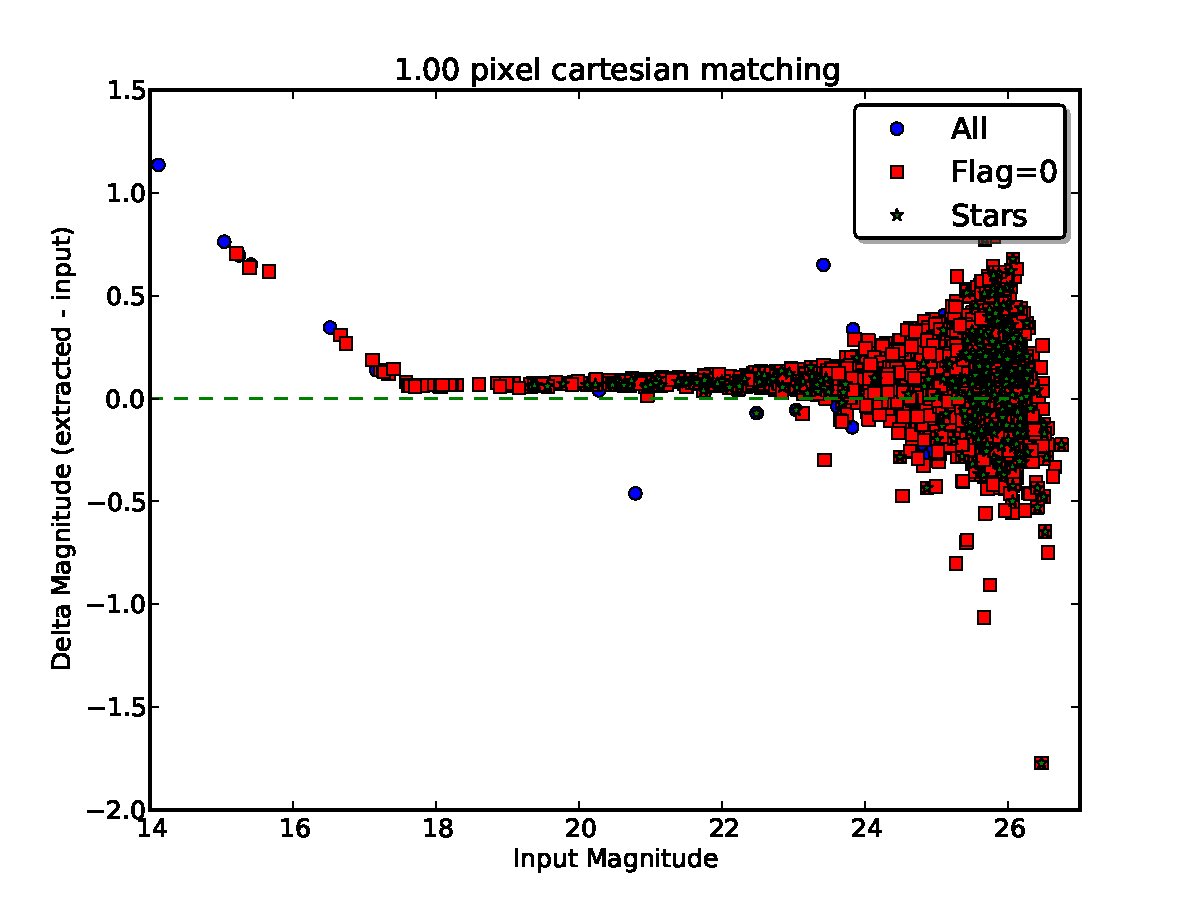
\includegraphics{Magnitudes15.pdf}
\caption{Example showing the recovered photometry from a reference simulator image with realistic noise, average background,
and end-of-life radiation damage, but without aperture correction. The offset is about 0.08mag.}\end{figure}
\begin{figure}[htbp]
\centering
\capstart

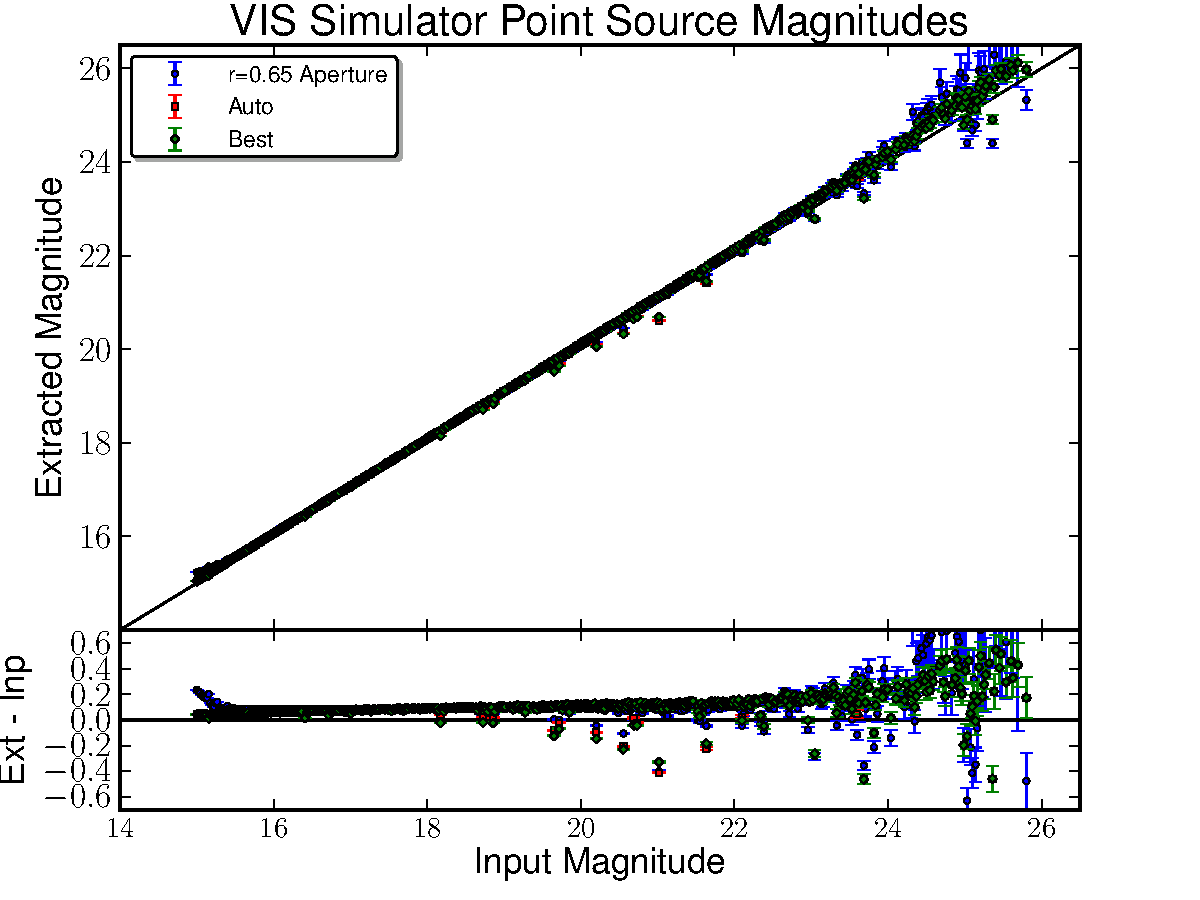
\includegraphics{magnitudes.pdf}
\caption{Example showing the recovered photometry for point sources from a reference simulator image with realistic noise
and an average background, but without any radiation damage to the CCD.}\end{figure}


\chapter{Indices and tables}
\label{index:indices-and-tables}\begin{itemize}
\item {} 
\emph{genindex}

\item {} 
\emph{modindex}

\item {} 
\emph{search}

\end{itemize}


\renewcommand{\indexname}{Python Module Index}
\begin{theindex}
\def\bigletter#1{{\Large\sffamily#1}\nopagebreak\vspace{1mm}}
\bigletter{a}
\item {\texttt{analysis.analyse}}, \pageref{analysis:module-analysis.analyse}
\item {\texttt{analysis.analyseGhosts}}, \pageref{reduction:module-analysis.analyseGhosts}
\item {\texttt{analysis.analyseSpotMeasurements}}, \pageref{analysis:module-analysis.analyseSpotMeasurements}
\item {\texttt{analysis.biasCalibration}}, \pageref{reduction:module-analysis.biasCalibration}
\item {\texttt{analysis.cosmicrayCalibration}}, \pageref{reduction:module-analysis.cosmicrayCalibration}
\item {\texttt{analysis.CTIpower}}, \pageref{analysis:module-analysis.CTIpower}
\item {\texttt{analysis.fitPSF}}, \pageref{analysis:module-analysis.fitPSF}
\item {\texttt{analysis.FlatfieldCalibration}}, \pageref{reduction:module-analysis.FlatfieldCalibration}
\item {\texttt{analysis.nonlinearityCalibration}}, \pageref{reduction:module-analysis.nonlinearityCalibration}
\item {\texttt{analysis.nonlinearityModelTransfer}}, \pageref{analysis:module-analysis.nonlinearityModelTransfer}
\item {\texttt{analysis.PSFbasisSets}}, \pageref{analysis:module-analysis.PSFbasisSets}
\item {\texttt{analysis.PSFproperties}}, \pageref{analysis:module-analysis.PSFproperties}
\item {\texttt{analysis.shape}}, \pageref{analysis:module-analysis.shape}
\item {\texttt{analysis.sourceFinder}}, \pageref{analysis:module-analysis.sourceFinder}
\item {\texttt{analysis.testCTIcorrection}}, \pageref{reduction:module-analysis.testCTIcorrection}
\indexspace
\bigletter{e}
\item {\texttt{ETC.ETC}}, \pageref{ETC:module-ETC.ETC}
\indexspace
\bigletter{p}
\item {\texttt{postproc.postprocessing}}, \pageref{postproc:module-postproc.postprocessing}
\item {\texttt{postproc.tileCCD}}, \pageref{postproc:module-postproc.tileCCD}
\item {\texttt{postproc.tileFPA}}, \pageref{postproc:module-postproc.tileFPA}
\indexspace
\bigletter{r}
\item {\texttt{reduction.reduceVISdata}}, \pageref{reduction:module-reduction.reduceVISdata}
\indexspace
\bigletter{s}
\item {\texttt{sandbox.MTF}}, \pageref{instrument:module-sandbox.MTF}
\item {\texttt{simulator.generateGalaxies}}, \pageref{simulator:module-simulator.generateGalaxies}
\item {\texttt{simulator.simulator}}, \pageref{simulator:module-simulator.simulator}
\item {\texttt{sources.createObjectCatalogue}}, \pageref{sources:module-sources.createObjectCatalogue}
\item {\texttt{sources.generatePostageStamps}}, \pageref{sources:module-sources.generatePostageStamps}
\item {\texttt{support.VISinstrumentModel}}, \pageref{instrument:module-support.VISinstrumentModel}
\end{theindex}

\renewcommand{\indexname}{Index}
\printindex
\end{document}
